\documentclass[11pt]{article}
%l !Rnw weave = knitr

%% ===== Document Encoding and Fonts =====
\usepackage[utf8]{inputenc}
\usepackage[T1]{fontenc}
\usepackage{crimson}

%% ===== Page Layout =====
\usepackage{geometry}
\geometry{verbose,tmargin=1in,bmargin=1in,lmargin=1in,rmargin=1in}
\usepackage{setspace}

%% ===== Graphics and Colors =====
\usepackage{graphicx}
\usepackage{color}
\usepackage{tikz}
\usepackage{epstopdf}
\usepackage{rotating}

% Image handling rules
\epstopdfDeclareGraphicsRule{.tif}{png}{.png}{convert #1 \OutputFile}
\AppendGraphicsExtensions{.tif}

% Maxwidth for images
\makeatletter
\def\maxwidth{%
  \ifdim\Gin@nat@width>\linewidth
    \linewidth
  \else
    \Gin@nat@width
  \fi
}
\makeatother

% Float settings
\usepackage{float}
\renewcommand{\textfraction}{0.05}
\renewcommand{\topfraction}{0.8}
\renewcommand{\bottomfraction}{0.8}
\renewcommand{\floatpagefraction}{0.75}

%% ===== Math Packages =====
\usepackage{amsmath,amsfonts,amssymb,amsthm}
\setcounter{MaxMatrixCols}{10}
\newcommand{\Expect}{{\rm I\kern-.3em E}} % Expectation operator

%% ===== Tables and Figures =====
\usepackage{array}
\usepackage{booktabs}
\usepackage{dcolumn}
\usepackage{multirow}
\usepackage{subcaption}
\usepackage{threeparttable}
\usepackage{tabulary}
\newcolumntype{M}[1]{>{\centering\arraybackslash}m{#1}}

%% ===== Links and URLs =====
\usepackage{url}
\usepackage{hyperref}
\hypersetup{
    colorlinks=true,
    breaklinks=true,
    allcolors=[RGB]{128,0,0}
}

%% ===== Bibliography =====
\usepackage{natbib}

%% ===== Miscellaneous Packages =====
\usepackage{seqsplit}
\usepackage{soul}
\usepackage{bbding} % checkmark symbol
\usepackage{comment}
\usepackage{alltt}

%% ===== Code Highlighting =====
\definecolor{fgcolor}{rgb}{0.345, 0.345, 0.345}
\definecolor{shadecolor}{rgb}{.97, .97, .97}
\definecolor{messagecolor}{rgb}{0, 0, 0}
\definecolor{warningcolor}{rgb}{1, 0, 1}
\definecolor{errorcolor}{rgb}{1, 0, 0}

\newcommand{\hlnum}[1]{\textcolor[rgb]{0.686,0.059,0.569}{#1}}%
\newcommand{\hlstr}[1]{\textcolor[rgb]{0.192,0.494,0.8}{#1}}%
\newcommand{\hlcom}[1]{\textcolor[rgb]{0.678,0.584,0.686}{\textit{#1}}}%
\newcommand{\hlopt}[1]{\textcolor[rgb]{0,0,0}{#1}}%
\newcommand{\hlstd}[1]{\textcolor[rgb]{0.345,0.345,0.345}{#1}}%
\newcommand{\hlkwa}[1]{\textcolor[rgb]{0.161,0.373,0.58}{\textbf{#1}}}%
\newcommand{\hlkwb}[1]{\textcolor[rgb]{0.69,0.353,0.396}{#1}}%
\newcommand{\hlkwc}[1]{\textcolor[rgb]{0.333,0.667,0.333}{#1}}%
\newcommand{\hlkwd}[1]{\textcolor[rgb]{0.737,0.353,0.396}{\textbf{#1}}}%

%% ===== Knitr Environment =====
\usepackage{framed}
\makeatletter
\newenvironment{kframe}{%
 \def\at@end@of@kframe{}%
 \ifinner\ifhmode%
  \def\at@end@of@kframe{\end{minipage}}%
  \begin{minipage}{\columnwidth}%
 \fi\fi%
 \def\FrameCommand##1{\hskip\@totalleftmargin \hskip-\fboxsep
 \colorbox{shadecolor}{##1}\hskip-\fboxsep
     % There is no \\@totalrightmargin, so:
     \hskip-\linewidth \hskip-\@totalleftmargin \hskip\columnwidth}%
 \MakeFramed {\advance\hsize-\width
   \@totalleftmargin\z@ \linewidth\hsize
   \@setminipage}}%
 {\par\unskip\endMakeFramed%
 \at@end@of@kframe}
\makeatother
\newenvironment{knitrout}{}{} % an empty environment to be redefined in TeX

%% ===== Custom Footnote Handling =====
\let\oldFootnote\footnote
\newcommand\nextToken\relax

\renewcommand\footnote[1]{%
    \oldFootnote{#1}\futurelet\nextToken\isFootnote}

\newcommand\isFootnote{%
    \ifx\footnote\nextToken\textsuperscript{,}\fi}

%% ===== Theorem-like Environments =====
\theoremstyle{plain}
\newtheorem{thm}{\protect\theoremname}
\newtheorem{prop}{\protect\propositionname}
\newtheorem{theorem}{{Theorem}}
\newtheorem{proposition}[theorem]{Proposition}
\newtheorem{lemma}[theorem]{Lemma}
\newtheorem{definition}[theorem]{Definition}
\newtheorem{prediction}{Prediction}
\newtheorem{open_question}{Open question}
\newtheorem{assumption}[theorem]{Assumption}
\newtheorem{observation}[theorem]{Observation}
\newtheorem{claim}[theorem]{{Claim}}
\newtheorem{example}[theorem]{{Example}}
\newtheorem{corollary}[theorem]{{Corollary}}
\newtheorem{remark}[theorem]{{Remark}}
\newtheorem{assumptions}[theorem]{{Assumptions}}
\newtheorem*{thm1star}{{Theorem $\mathbf{1^*}$}}
\newtheorem*{thm2star}{{Theorem $\mathbf{2^*}$}}
\newtheorem*{theorem*}{Theorem}
\newtheorem*{lemma*}{Lemma}

%% ===== Hypothesis Environments =====
\newtheorem{hyp}{Hypothesis}
\makeatletter
\newcounter{subhyp}
\let\savedc@hyp\c@hyp
\newenvironment{subhyp}
 {%
  \setcounter{subhyp}{0}%
  \stepcounter{hyp}%
  \edef\saved@hyp{\thehyp}% Save the current value of hyp
  \let\c@hyp\c@subhyp     % Now hyp is subhyp
  \renewcommand{\thehyp}{\saved@hyp\alph{hyp}}%
 }
 {}
\newcommand{\normhyp}{%
  \let\c@hyp\savedc@hyp % revert to the old one
  \renewcommand\thehyp{\arabic{hyp}}%
}
\makeatother

%% ===== Custom Macros =====
\providecommand{\examplename}{Example}
\providecommand{\propositionname}{Proposition}
\providecommand{\theoremname}{Theorem}
\newcommand{\bi}{\begin{itemize}}
\newcommand{\ei}{\end{itemize}}
\newcommand{\bb}{\begin{block}}
\newcommand{\eb}{\end{block}}
\newcommand{\bmath}{\begin{eqnarray}}
\newcommand{\emath}{\end{eqnarray}}
\newcommand{\bmathnn}{\begin{eqnarray*}}
\newcommand{\emathnn}{\end{eqnarray*}}

%% ===== Statistical Significance Markers =====
\newcommand*{\SuperScriptSameStyle}[1]{%
  \ensuremath{%
    \mathchoice
      {{}^{\displaystyle #1}}%
      {{}^{\textstyle #1}}%
      {{}^{\scriptstyle #1}}%
      {{}^{\scriptscriptstyle #1}}%
  }%
}

\newcommand*{\oneS}{\SuperScriptSameStyle{*}}
\newcommand*{\twoS}{\SuperScriptSameStyle{**}}
\newcommand*{\threeS}{\SuperScriptSameStyle{*{*}*}}
\newcommand{\vh}[1]{\textcolor{red}{(VH: #1)}}

%% ===== Other Settings =====
\IfFileExists{upquote.sty}{\usepackage{upquote}}{}

\usetikzlibrary{arrows.meta, positioning, fit, backgrounds, calc, shapes.geometric, decorations.pathmorphing}

\begin{document}

\title{The Youth Dividend: Political Impacts of Demographic Transitions}

\author{
\textbf{R\'{e}dha Chaba} \\ LEMMA -- Paris-Panthéon-Assas  \\
\and \textbf{Michael T. Dorsch}
  \\ CEU -- Vienna 
\and \textbf{Victor Hiller} \\ LEMMA -- Paris-Panthéon-Assas \\ 
\and \textbf{Paul Maarek}   \\ LEMMA -- Paris-Panthéon-Assas  \\  
}
\date{\today}

\maketitle
\tableofcontents
\section{Regressions}
\subsection{Polity}
\subsubsection{Baseline Results}

\begin{table}[H]
\sffamily
\caption{{Baseline results -- $\Delta$ Polity2 $\ge$ 2}}
\resizebox{17cm}{!}{
\begin{tabular}{@{\extracolsep{5pt}} l c c c c c c c}
\\
\toprule
\toprule

& \multicolumn{7}{c}{{Binary DV:  $\Delta$ Polity2 $\ge$ 2}}\\
\cmidrule(r){2-8}

& \multicolumn{1}{c}{{OLS}}& \multicolumn{2}{c}{{Own fertility}}  &  \multicolumn{2}{c}{{Neighbors' fertility}} &  \multicolumn{2}{c}{{SPEI}}  \\
	  \cmidrule(r){2-2}
	  \cmidrule(r){3-4}
	  \cmidrule(r){5-6}
  	  \cmidrule(r){7-8}
	  
 & &  \multicolumn{1}{c}{{RF}}  & \multicolumn{1}{c}{{2SLS}} &  \multicolumn{1}{c}{{RF}}  & \multicolumn{1}{c}{{2SLS}}&  \multicolumn{1}{c}{{RF}}  & \multicolumn{1}{c}{{2SLS}}\\
 	  \cmidrule(r){3-3}
      \cmidrule(r){4-4}
      \cmidrule(r){5-5}
      \cmidrule(r){6-6}
      \cmidrule(r){7-7}
      \cmidrule(r){8-8}

 & \multicolumn{1}{c}{{(1)}} &  \multicolumn{1}{c}{{(2)}}  & \multicolumn{1}{c}{{(3)}} &  \multicolumn{1}{c}{{(4)}} & \multicolumn{1}{c}{{(5)}} & \multicolumn{1}{c}{(6)} &  \multicolumn{1}{c}{{(7)}}\\
 \midrule  
   Youth ratio (15 - 19)$_{t-1}$ &       0.355** &               &       0.697***&               &       1.362** &               &       2.886** \\
   \smallskip
            &      (0.15)   &               &      (0.26)   &               &      (0.68)   &               &      (1.46)   \\
   Net fertility rate$_{t-16}$  &               &       0.002** &               &               &               &               &               \\
   \smallskip
            &               &      (0.00)   &               &               &               &               &               \\
   Neighbors' net fertility$_{t-21}$&               &               &               &       0.003** &               &               &               \\
   \smallskip
            &               &               &               &      (0.00)   &               &               &               \\
   SPEI $\times$ Agriculture GDP share$_{t-17}$&               &               &               &               &               &      -0.099***&               \\
   \smallskip
            &               &               &               &               &               &      (0.03)   &               \\
SPEI$_{t-17}$&               &               &               &               &               &       0.014   &               \\
\medskip
            &               &               &               &               &               &      (0.01)   &               \\

Standard controls  & \checkmark & \checkmark & \checkmark & \checkmark & \checkmark & \checkmark & \checkmark  \\
\smallskip
Country \& year FE's & \checkmark & \checkmark & \checkmark & \checkmark  & \checkmark & \checkmark & \checkmark  \\
K-P F-stat on excl. IV's&       --        &        --      &     328.751   &         --      &      50.009   &         --      &       7.283   \\

Observations&       8,608   &       6,478   &       6,478   &       5,368   &       5,367   &       6,697   &       6,697   \\
Countries   &         154   &         154   &         154   &         153   &         152   &         142   &         142   \\
Within-R$^2$&       0.037   &       0.052   &       --        &       0.057   &         --      &       0.049   &        --       \\
\bottomrule
\multicolumn{8}{p{19cm}}{\footnotesize \emph{Notes}:   Robust standard errors clustered by country are in parentheses.  The standard set of controls includes once lagged values of: the log of GDP per capita, the growth rate of GDP per capita, and  the Polity score.  Referring to the Kleibergen-Paap (K-P) F-statistic, the test's null hypothesis is that the set of instruments is weak.  {The panel runs from 1951 -- 2017 for the specifications that do not include the 16-year lagged fertility rates and from 1973 -- 2017 for the specifications that do include the 16-year lagged fertility rates.}   *** / ** / * represent significance at the 0.01 / 0.05 / 0.10 levels, respectively.}
\end{tabular}
}
\end{table}





\begin{table}[H]
\sffamily
\caption{{Baseline results -- $\Delta$ Polity2 $\ge$ 1}}
\resizebox{17cm}{!}{
\begin{tabular}{@{\extracolsep{5pt}} l c c c c c c c}
\\
\toprule
\toprule

& \multicolumn{7}{c}{{Binary DV:  $\Delta$ Polity2 $\ge$ 1}}\\
\cmidrule(r){2-8}

& \multicolumn{1}{c}{{OLS}}& \multicolumn{2}{c}{{Own fertility}}  &  \multicolumn{2}{c}{{Neighbors' fertility}} &  \multicolumn{2}{c}{{SPEI}}  \\
	  \cmidrule(r){2-2}
	  \cmidrule(r){3-4}
	  \cmidrule(r){5-6}
  	  \cmidrule(r){7-8}
	  
 & &  \multicolumn{1}{c}{{RF}}  & \multicolumn{1}{c}{{2SLS}} &  \multicolumn{1}{c}{{RF}}  & \multicolumn{1}{c}{{2SLS}}&  \multicolumn{1}{c}{{RF}}  & \multicolumn{1}{c}{{2SLS}}\\
 	  \cmidrule(r){3-3}
      \cmidrule(r){4-4}
      \cmidrule(r){5-5}
      \cmidrule(r){6-6}
      \cmidrule(r){7-7}
      \cmidrule(r){8-8}

 & \multicolumn{1}{c}{{(1)}} &  \multicolumn{1}{c}{{(2)}}  & \multicolumn{1}{c}{{(3)}} &  \multicolumn{1}{c}{{(4)}} & \multicolumn{1}{c}{{(5)}} & \multicolumn{1}{c}{(6)} &  \multicolumn{1}{c}{{(7)}}\\
 \midrule  
   Youth ratio (15 - 19)$_{t-1}$ &       0.525***&               &       0.959***&               &       2.620***&               &       4.431** \\
   \smallskip
            &      (0.20)   &               &      (0.32)   &               &      (0.85)   &               &      (1.97)   \\
   Net fertility rate$_{t-16}$  &               &       0.003***&               &               &               &               &               \\
   \smallskip
            &               &      (0.00)   &               &               &               &               &               \\
   Neighbors' net fertility$_{t-21}$&               &               &               &       0.006***&               &               &               \\
   \smallskip
            &               &               &               &      (0.00)   &               &               &               \\
   SPEI $\times$ Agriculture GDP share$_{t-17}$&               &               &               &               &               &      -0.133***&               \\
   \smallskip
            &               &               &               &               &               &      (0.04)   &               \\
SPEI$_{t-17}$&               &               &               &               &               &       0.016   &               \\
\medskip
            &               &               &               &               &               &      (0.01)   &               \\

Standard controls  & \checkmark & \checkmark & \checkmark & \checkmark & \checkmark & \checkmark & \checkmark  \\
\smallskip
Country \& year FE's & \checkmark & \checkmark & \checkmark & \checkmark  & \checkmark & \checkmark & \checkmark  \\
K-P F-stat on excl. IV's&       --        &        --      &     328.751   &         --      &      50.009   &         --      &       7.283   \\

Observations&       8,608   &       6,478   &       6,478   &       5,368   &       5,367   &       6,697   &       6,697   \\
Countries   &         154   &         154   &         154   &         153   &         152   &         142   &         142   \\
Within-R$^2$&       0.040   &       0.052   &       --        &       0.061   &        --       &       0.048   &    --           \\
\bottomrule
\multicolumn{8}{p{19cm}}{\footnotesize \emph{Notes}:   Robust standard errors clustered by country are in parentheses.  The standard set of controls includes once lagged values of: the log of GDP per capita, the growth rate of GDP per capita, and  the Polity score.  Referring to the Kleibergen-Paap (K-P) F-statistic, the test's null hypothesis is that the set of instruments is weak.  {The panel runs from 1951 -- 2017 for the specifications that do not include the 16-year lagged fertility rates and from 1973 -- 2017 for the specifications that do include the 16-year lagged fertility rates.}   *** / ** / * represent significance at the 0.01 / 0.05 / 0.10 levels, respectively.}
\end{tabular}
}
\end{table}





\begin{table}[H]
\sffamily
\caption{{Baseline results -- $\Delta$ Polity2 $\ge$ 3}}
\resizebox{17cm}{!}{
\begin{tabular}{@{\extracolsep{5pt}} l c c c c c c c}
\\
\toprule
\toprule

& \multicolumn{7}{c}{{Binary DV:  $\Delta$ Polity2 $\ge$ 3}}\\
\cmidrule(r){2-8}

& \multicolumn{1}{c}{{OLS}}& \multicolumn{2}{c}{{Own fertility}}  &  \multicolumn{2}{c}{{Neighbors' fertility}} &  \multicolumn{2}{c}{{SPEI}}  \\
	  \cmidrule(r){2-2}
	  \cmidrule(r){3-4}
	  \cmidrule(r){5-6}
  	  \cmidrule(r){7-8}
	  
 & &  \multicolumn{1}{c}{{RF}}  & \multicolumn{1}{c}{{2SLS}} &  \multicolumn{1}{c}{{RF}}  & \multicolumn{1}{c}{{2SLS}}&  \multicolumn{1}{c}{{RF}}  & \multicolumn{1}{c}{{2SLS}}\\
 	  \cmidrule(r){3-3}
      \cmidrule(r){4-4}
      \cmidrule(r){5-5}
      \cmidrule(r){6-6}
      \cmidrule(r){7-7}
      \cmidrule(r){8-8}

 & \multicolumn{1}{c}{{(1)}} &  \multicolumn{1}{c}{{(2)}}  & \multicolumn{1}{c}{{(3)}} &  \multicolumn{1}{c}{{(4)}} & \multicolumn{1}{c}{{(5)}} & \multicolumn{1}{c}{(6)} &  \multicolumn{1}{c}{{(7)}}\\
 \midrule  
   Youth ratio (15 - 19)$_{t-1}$ &       0.355***&               &       0.543** &               &       1.115** &               &       1.301   \\
            \smallskip
            &      (0.12)   &               &      (0.21)   &               &      (0.50)   &               &      (0.99)   \\
   Net fertility rate$_{t-16}$ &               &       0.002** &               &               &               &               &               \\
            \smallskip
            &               &      (0.00)   &               &               &               &               &               \\
   Neighbors' net fertility$_{t-21}$&               &               &               &       0.002** &               &               &               \\
            \smallskip
            &               &               &               &      (0.00)   &               &               &               \\
   SPEI $\times$ Agriculture GDP share$_{t-17}$&               &               &               &               &               &      -0.046*  &               \\
            \smallskip
            &               &               &               &               &               &      (0.03)   &               \\
SPEI$_{t-17}$&               &               &               &               &               &       0.007   &               \\
            \medskip
            &               &               &               &               &               &      (0.01)   &               \\

Standard controls  & \checkmark & \checkmark & \checkmark & \checkmark & \checkmark & \checkmark & \checkmark  \\
\smallskip
Country \& year FE's & \checkmark & \checkmark & \checkmark & \checkmark  & \checkmark & \checkmark & \checkmark  \\
K-P F-stat on excl. IV's&       --        &        --      &     328.751   &         --      &      50.009   &         --      &       7.283   \\

Observations&       8,608   &       6,478   &       6,478   &       5,368   &       5,367   &       6,697   &       6,697   \\
Countries   &         154   &         154   &         154   &         153   &         152   &         142   &         142   \\
Within-R$^2$&       0.037   &       0.053   &        --       &       0.061   &     --          &       0.046   &         --      \\
\bottomrule
\multicolumn{8}{p{19cm}}{\footnotesize \emph{Notes}:   Robust standard errors clustered by country are in parentheses.  The standard set of controls includes once lagged values of: the log of GDP per capita, the growth rate of GDP per capita, and  the Polity score.  Referring to the Kleibergen-Paap (K-P) F-statistic, the test's null hypothesis is that the set of instruments is weak.  {The panel runs from 1951 -- 2017 for the specifications that do not include the 16-year lagged fertility rates and from 1973 -- 2017 for the specifications that do include the 16-year lagged fertility rates.}   *** / ** / * represent significance at the 0.01 / 0.05 / 0.10 levels, respectively.}
\end{tabular}
}
\end{table}

\begin{table}[H]
\sffamily
\caption{{Baseline results -- $\Delta$ Polity2}}
\resizebox{17cm}{!}{
\begin{tabular}{@{\extracolsep{5pt}} l c c c c c c c}
\\
\toprule
\toprule

& \multicolumn{7}{c}{{Continuous DV:  $\Delta$ Polity2}}\\
\cmidrule(r){2-8}

& \multicolumn{1}{c}{{OLS}}& \multicolumn{2}{c}{{Own fertility}}  &  \multicolumn{2}{c}{{Neighbors' fertility}} &  \multicolumn{2}{c}{{SPEI}}  \\
	  \cmidrule(r){2-2}
	  \cmidrule(r){3-4}
	  \cmidrule(r){5-6}
  	  \cmidrule(r){7-8}
	  
 & &  \multicolumn{1}{c}{{RF}}  & \multicolumn{1}{c}{{2SLS}} &  \multicolumn{1}{c}{{RF}}  & \multicolumn{1}{c}{{2SLS}}&  \multicolumn{1}{c}{{RF}}  & \multicolumn{1}{c}{{2SLS}}\\
 	  \cmidrule(r){3-3}
      \cmidrule(r){4-4}
      \cmidrule(r){5-5}
      \cmidrule(r){6-6}
      \cmidrule(r){7-7}
      \cmidrule(r){8-8}

 & \multicolumn{1}{c}{{(1)}} &  \multicolumn{1}{c}{{(2)}}  & \multicolumn{1}{c}{{(3)}} &  \multicolumn{1}{c}{{(4)}} & \multicolumn{1}{c}{{(5)}} & \multicolumn{1}{c}{(6)} &  \multicolumn{1}{c}{{(7)}}\\
 \midrule  
   Youth ratio (15 - 19)$_{t-1}$ &       3.984***&               &       5.995***&               &      12.085***&               &      23.505** \\
   \smallskip
            &      (1.34)   &               &      (1.99)   &               &      (4.42)   &               &     (11.60)   \\
   Net fertility rate$_{t-16}$  &               &       0.018***&               &               &               &               &               \\
            \smallskip
            &               &      (0.01)   &               &               &               &               &               \\
   Neighbors' net fertility$_{t-21}$&               &               &               &       0.026***&               &               &               \\
            \smallskip
            &               &               &               &      (0.01)   &               &               &               \\
   SPEI $\times$ Agriculture GDP share$_{t-17}$&               &               &               &               &               &      -0.492** &               \\
            \smallskip
            &               &               &               &               &               &      (0.24)   &               \\
SPEI$_{t-17}$&               &               &               &               &               &       0.014   &               \\
            \medskip
            &               &               &               &               &               &      (0.08)   &               \\

Standard controls  & \checkmark & \checkmark & \checkmark & \checkmark & \checkmark & \checkmark & \checkmark  \\
\smallskip
Country \& year FE's & \checkmark & \checkmark & \checkmark & \checkmark  & \checkmark & \checkmark & \checkmark  \\
K-P F-stat on excl. IV's&       --        &        --      &     328.751   &         --      &      50.009   &         --      &       7.283   \\

Observations&       8,608   &       6,478   &       6,478   &       5,368   &       5,367   &       6,697   &       6,697   \\
Countries   &         154   &         154   &         154   &         153   &         152   &         142   &         142   \\
Within-R$^2$&       0.067   &       0.076   &       --        &       0.083   &       --        &       0.075   &         --      \\
\bottomrule
\multicolumn{8}{p{19cm}}{\footnotesize \emph{Notes}:   Robust standard errors clustered by country are in parentheses.  The standard set of controls includes once lagged values of: the log of GDP per capita, the growth rate of GDP per capita, and  the Polity score.  Referring to the Kleibergen-Paap (K-P) F-statistic, the test's null hypothesis is that the set of instruments is weak.  {The panel runs from 1951 -- 2017 for the specifications that do not include the 16-year lagged fertility rates and from 1973 -- 2017 for the specifications that do include the 16-year lagged fertility rates.}   *** / ** / * represent significance at the 0.01 / 0.05 / 0.10 levels, respectively.}
\end{tabular}
}
\end{table}


\begin{table}[H]
\sffamily
\caption{{Baseline results -- $\Delta$ Polity2 $>$ 0}}
\resizebox{17cm}{!}{
\begin{tabular}{@{\extracolsep{5pt}} l c c c c c c c}
\\
\toprule
\toprule

& \multicolumn{7}{c}{{Continuous DV:  $\Delta$ Polity2 $>$ 0}}\\
\cmidrule(r){2-8}

& \multicolumn{1}{c}{{OLS}}& \multicolumn{2}{c}{{Own fertility}}  &  \multicolumn{2}{c}{{Neighbors' fertility}} &  \multicolumn{2}{c}{{SPEI}}  \\
	  \cmidrule(r){2-2}
	  \cmidrule(r){3-4}
	  \cmidrule(r){5-6}
  	  \cmidrule(r){7-8}
	  
 & &  \multicolumn{1}{c}{{RF}}  & \multicolumn{1}{c}{{2SLS}} &  \multicolumn{1}{c}{{RF}}  & \multicolumn{1}{c}{{2SLS}}&  \multicolumn{1}{c}{{RF}}  & \multicolumn{1}{c}{{2SLS}}\\
 	  \cmidrule(r){3-3}
      \cmidrule(r){4-4}
      \cmidrule(r){5-5}
      \cmidrule(r){6-6}
      \cmidrule(r){7-7}
      \cmidrule(r){8-8}

 & \multicolumn{1}{c}{{(1)}} &  \multicolumn{1}{c}{{(2)}}  & \multicolumn{1}{c}{{(3)}} &  \multicolumn{1}{c}{{(4)}} & \multicolumn{1}{c}{{(5)}} & \multicolumn{1}{c}{(6)} &  \multicolumn{1}{c}{{(7)}}\\
 \midrule  
   Youth ratio (15 - 19)$_{t-1}$ &       1.777*  &               &       4.028***&               &      10.084***&               &      15.915*  \\
   \smallskip
            &      (0.91)   &               &      (1.53)   &               &      (3.80)   &               &      (8.54)   \\
   Net fertility rate$_{t-16}$  &               &       0.012** &               &               &               &               &               \\
            \smallskip
            &               &      (0.00)   &               &               &               &               &               \\
   Neighbors' net fertility$_{t-21}$&               &               &               &       0.021***&               &               &               \\
            \smallskip
            &               &               &               &      (0.01)   &               &               &               \\
   SPEI $\times$ Agriculture GDP share$_{t-17}$&               &               &               &               &               &      -0.467** &               \\
            \smallskip
            &               &               &               &               &               &      (0.18)   &               \\
SPEI$_{t-17}$&               &               &               &               &               &       0.053   &               \\
            \medskip
            &               &               &               &               &               &      (0.06)   &               \\

Standard controls  & \checkmark & \checkmark & \checkmark & \checkmark & \checkmark & \checkmark & \checkmark  \\
\smallskip
Country \& year FE's & \checkmark & \checkmark & \checkmark & \checkmark  & \checkmark & \checkmark & \checkmark  \\
K-P F-stat on excl. IV's&       --        &        --      &     328.751   &         --      &      50.009   &         --      &       7.283   \\

Observations&       8,608   &       6,478   &       6,478   &       5,368   &       5,367   &       6,697   &       6,697   \\
Countries   &         154   &         154   &         154   &         153   &         152   &         142   &         142   \\
Within-R$^2$&       0.046   &       0.067   &         --      &       0.077   &        --       &       0.056   &        --       \\
\bottomrule
\multicolumn{8}{p{19cm}}{\footnotesize \emph{Notes}:   Robust standard errors clustered by country are in parentheses.  The standard set of controls includes once lagged values of: the log of GDP per capita, the growth rate of GDP per capita, and  the Polity score.  Referring to the Kleibergen-Paap (K-P) F-statistic, the test's null hypothesis is that the set of instruments is weak.  {The panel runs from 1951 -- 2017 for the specifications that do not include the 16-year lagged fertility rates and from 1973 -- 2017 for the specifications that do include the 16-year lagged fertility rates.}   *** / ** / * represent significance at the 0.01 / 0.05 / 0.10 levels, respectively.}
\end{tabular}
}
\end{table}









\subsubsection{Drop Polity $\ge$ 8 -- 32.2\% Obs. Dropped}

\begin{table}[H]
\sffamily
\caption{{Drop Polity $\ge$ 8 -- $\Delta$ Polity2 $\ge$ 2}}
\resizebox{17cm}{!}{
\begin{tabular}{@{\extracolsep{5pt}} l c c c c c c c}
\\
\toprule
\toprule

& \multicolumn{7}{c}{{Binary DV:  $\Delta$ Polity2 $\ge$ 2}}\\
\cmidrule(r){2-8}

& \multicolumn{1}{c}{{OLS}}& \multicolumn{2}{c}{{Own fertility}}  &  \multicolumn{2}{c}{{Neighbors' fertility}} &  \multicolumn{2}{c}{{SPEI}}  \\
	  \cmidrule(r){2-2}
	  \cmidrule(r){3-4}
	  \cmidrule(r){5-6}
  	  \cmidrule(r){7-8}
	  
 & &  \multicolumn{1}{c}{{RF}}  & \multicolumn{1}{c}{{2SLS}} &  \multicolumn{1}{c}{{RF}}  & \multicolumn{1}{c}{{2SLS}}&  \multicolumn{1}{c}{{RF}}  & \multicolumn{1}{c}{{2SLS}}\\
 	  \cmidrule(r){3-3}
      \cmidrule(r){4-4}
      \cmidrule(r){5-5}
      \cmidrule(r){6-6}
      \cmidrule(r){7-7}
      \cmidrule(r){8-8}

 & \multicolumn{1}{c}{{(1)}} &  \multicolumn{1}{c}{{(2)}}  & \multicolumn{1}{c}{{(3)}} &  \multicolumn{1}{c}{{(4)}} & \multicolumn{1}{c}{{(5)}} & \multicolumn{1}{c}{(6)} &  \multicolumn{1}{c}{{(7)}}\\
 \midrule  
   Youth ratio (15 - 19)$_{t-1}$ &      -0.037   &               &      -0.216   &               &      -0.576   &               &       0.554   \\
            &      (0.22)   &               &      (0.35)   &               &      (1.03)   &               &      (1.62)   \\
   Net fertility rate$_{t-16}$  &               &      -0.001   &               &               &               &               &               \\
            &               &      (0.00)   &               &               &               &               &               \\
   Neighbors' net fertility$_{t-21}$&               &               &               &      -0.001   &               &               &               \\
            &               &               &               &      (0.00)   &               &               &               \\
   SPEI $\times$ Agriculture GDP share$_{t-17}$&               &               &               &               &               &      -0.110***&               \\
            &               &               &               &               &               &      (0.04)   &               \\
SPEI$_{t-17}$&               &               &               &               &               &       0.030*  &               \\
            &               &               &               &               &               &      (0.02)   &               \\
Standard controls  & \checkmark & \checkmark & \checkmark & \checkmark & \checkmark & \checkmark & \checkmark  \\
\smallskip
Country \& year FE's & \checkmark & \checkmark & \checkmark & \checkmark  & \checkmark & \checkmark & \checkmark  \\
K-P F-stat on excl. IV's&        --       &       --        &     175.194   &          --     &      39.267   &          --     &       5.503   \\

Observations&       5,727   &       4,174   &       4,174   &       3,374   &       3,373   &       4,493   &       4,493   \\
Countries   &         129   &         128   &         128   &         118   &         117   &         120   &         120   \\
Within-R$^2$&       0.041   &       0.048   &      --         &       0.053   &      --         &       0.047   &        --       \\
\bottomrule
\multicolumn{8}{p{19cm}}{\footnotesize \emph{Notes}:   Robust standard errors clustered by country are in parentheses.  The standard set of controls includes once lagged values of: the log of GDP per capita, the growth rate of GDP per capita, and  the Polity score.  Referring to the Kleibergen-Paap (K-P) F-statistic, the test's null hypothesis is that the set of instruments is weak.  {The panel runs from 1951 -- 2017 for the specifications that do not include the 16-year lagged fertility rates and from 1973 -- 2017 for the specifications that do include the 16-year lagged fertility rates.}   *** / ** / * represent significance at the 0.01 / 0.05 / 0.10 levels, respectively.}
\end{tabular}
}
\end{table}





\begin{table}[H]
\sffamily
\caption{{Drop Polity $\ge$ 8 -- $\Delta$ Polity2 $\ge$ 1}}
\resizebox{17cm}{!}{
\begin{tabular}{@{\extracolsep{5pt}} l c c c c c c c}
\\
\toprule
\toprule

& \multicolumn{7}{c}{{Binary DV:  $\Delta$ Polity2 $\ge$ 1}}\\
\cmidrule(r){2-8}

& \multicolumn{1}{c}{{OLS}}& \multicolumn{2}{c}{{Own fertility}}  &  \multicolumn{2}{c}{{Neighbors' fertility}} &  \multicolumn{2}{c}{{SPEI}}  \\
	  \cmidrule(r){2-2}
	  \cmidrule(r){3-4}
	  \cmidrule(r){5-6}
  	  \cmidrule(r){7-8}
	  
 & &  \multicolumn{1}{c}{{RF}}  & \multicolumn{1}{c}{{2SLS}} &  \multicolumn{1}{c}{{RF}}  & \multicolumn{1}{c}{{2SLS}}&  \multicolumn{1}{c}{{RF}}  & \multicolumn{1}{c}{{2SLS}}\\
 	  \cmidrule(r){3-3}
      \cmidrule(r){4-4}
      \cmidrule(r){5-5}
      \cmidrule(r){6-6}
      \cmidrule(r){7-7}
      \cmidrule(r){8-8}

 & \multicolumn{1}{c}{{(1)}} &  \multicolumn{1}{c}{{(2)}}  & \multicolumn{1}{c}{{(3)}} &  \multicolumn{1}{c}{{(4)}} & \multicolumn{1}{c}{{(5)}} & \multicolumn{1}{c}{(6)} &  \multicolumn{1}{c}{{(7)}}\\
 \midrule  
   Youth ratio (15 - 19)$_{t-1}$ &       0.009   &               &      -0.253   &               &       0.220   &               &       1.553   \\
            &      (0.29)   &               &      (0.41)   &               &      (1.05)   &               &      (2.05)   \\
   Net fertility rate$_{t-16}$  &               &      -0.001   &               &               &               &               &               \\
            &               &      (0.00)   &               &               &               &               &               \\
   Neighbors' net fertility$_{t-21}$&               &               &               &       0.001   &               &               &               \\
            &               &               &               &      (0.00)   &               &               &               \\
   SPEI $\times$ Agriculture GDP share$_{t-17}$&               &               &               &               &               &      -0.145***&               \\
            &               &               &               &               &               &      (0.05)   &               \\
SPEI$_{t-17}$&               &               &               &               &               &       0.034   &               \\
            &               &               &               &               &               &      (0.02)   &               \\

Standard controls  & \checkmark & \checkmark & \checkmark & \checkmark & \checkmark & \checkmark & \checkmark  \\
\smallskip
Country \& year FE's & \checkmark & \checkmark & \checkmark & \checkmark  & \checkmark & \checkmark & \checkmark  \\
K-P F-stat on excl. IV's&         --      &           --    &     175.194   &    --           &      39.267   &     --          &       5.503   \\

Observations&       5,727   &       4,174   &       4,174   &       3,374   &       3,373   &       4,493   &       4,493   \\
Countries   &         129   &         128   &         128   &         118   &         117   &         120   &         120   \\
Within-R$^2$&       0.050   &       0.054   &       --        &       0.063   &      --         &       0.053   &    --           \\
\bottomrule
\multicolumn{8}{p{19cm}}{\footnotesize \emph{Notes}:   Robust standard errors clustered by country are in parentheses.  The standard set of controls includes once lagged values of: the log of GDP per capita, the growth rate of GDP per capita, and  the Polity score.  Referring to the Kleibergen-Paap (K-P) F-statistic, the test's null hypothesis is that the set of instruments is weak.  {The panel runs from 1951 -- 2017 for the specifications that do not include the 16-year lagged fertility rates and from 1973 -- 2017 for the specifications that do include the 16-year lagged fertility rates.}   *** / ** / * represent significance at the 0.01 / 0.05 / 0.10 levels, respectively.}
\end{tabular}
}
\end{table}


\begin{table}[H]
\sffamily
\caption{{Drop Polity $\ge$ 8 -- $\Delta$ Polity2 $\ge$ 3}}
\resizebox{17cm}{!}{
\begin{tabular}{@{\extracolsep{5pt}} l c c c c c c c}
\\
\toprule
\toprule

& \multicolumn{7}{c}{{Binary DV:  $\Delta$ Polity2 $\ge$ 3}}\\
\cmidrule(r){2-8}

& \multicolumn{1}{c}{{OLS}}& \multicolumn{2}{c}{{Own fertility}}  &  \multicolumn{2}{c}{{Neighbors' fertility}} &  \multicolumn{2}{c}{{SPEI}}  \\
	  \cmidrule(r){2-2}
	  \cmidrule(r){3-4}
	  \cmidrule(r){5-6}
  	  \cmidrule(r){7-8}
	  
 & &  \multicolumn{1}{c}{{RF}}  & \multicolumn{1}{c}{{2SLS}} &  \multicolumn{1}{c}{{RF}}  & \multicolumn{1}{c}{{2SLS}}&  \multicolumn{1}{c}{{RF}}  & \multicolumn{1}{c}{{2SLS}}\\
 	  \cmidrule(r){3-3}
      \cmidrule(r){4-4}
      \cmidrule(r){5-5}
      \cmidrule(r){6-6}
      \cmidrule(r){7-7}
      \cmidrule(r){8-8}

 & \multicolumn{1}{c}{{(1)}} &  \multicolumn{1}{c}{{(2)}}  & \multicolumn{1}{c}{{(3)}} &  \multicolumn{1}{c}{{(4)}} & \multicolumn{1}{c}{{(5)}} & \multicolumn{1}{c}{(6)} &  \multicolumn{1}{c}{{(7)}}\\
 \midrule  
   Youth ratio (15 - 19)$_{t-1}$ &       0.112   &               &      -0.097   &               &      -0.468   &               &      -0.261   \\
            &      (0.17)   &               &      (0.26)   &               &      (0.74)   &               &      (1.37)   \\
   Net fertility rate$_{t-16}$ &               &      -0.000   &               &               &               &               &               \\
            &               &      (0.00)   &               &               &               &               &               \\
   Neighbors' net fertility$_{t-21}$&               &               &               &      -0.001   &               &               &               \\
            &               &               &               &      (0.00)   &               &               &               \\
   SPEI $\times$ Agriculture GDP share$_{t-17}$&               &               &               &               &               &      -0.048   &               \\
            &               &               &               &               &               &      (0.03)   &               \\
SPEI$_{t-17}$&               &               &               &               &               &       0.016   &               \\
            &               &               &               &               &               &      (0.01)   &               \\

Standard controls  & \checkmark & \checkmark & \checkmark & \checkmark & \checkmark & \checkmark & \checkmark  \\
\smallskip
Country \& year FE's & \checkmark & \checkmark & \checkmark & \checkmark  & \checkmark & \checkmark & \checkmark  \\
K-P F-stat on excl. IV's&        --       &         --      &     175.194   &       --        &      39.267   &         --      &       5.503   \\

Observations&       5,727   &       4,174   &       4,174   &       3,374   &       3,373   &       4,493   &       4,493   \\
Countries   &         129   &         128   &         128   &         118   &         117   &         120   &         120   \\
Within-R$^2$&       0.037   &       0.043   &       --        &       0.053   &        --       &       0.041   &       --        \\
\bottomrule
\multicolumn{8}{p{19cm}}{\footnotesize \emph{Notes}:   Robust standard errors clustered by country are in parentheses.  The standard set of controls includes once lagged values of: the log of GDP per capita, the growth rate of GDP per capita, and  the Polity score.  Referring to the Kleibergen-Paap (K-P) F-statistic, the test's null hypothesis is that the set of instruments is weak.  {The panel runs from 1951 -- 2017 for the specifications that do not include the 16-year lagged fertility rates and from 1973 -- 2017 for the specifications that do include the 16-year lagged fertility rates.}   *** / ** / * represent significance at the 0.01 / 0.05 / 0.10 levels, respectively.}
\end{tabular}
}
\end{table}


\begin{table}[H]
\sffamily
\caption{{Drop Polity $\ge$ 8 -- $\Delta$ Polity2}}
\resizebox{17cm}{!}{
\begin{tabular}{@{\extracolsep{5pt}} l c c c c c c c}
\\
\toprule
\toprule

& \multicolumn{7}{c}{{Continuous DV:  $\Delta$ Polity2}}\\
\cmidrule(r){2-8}

& \multicolumn{1}{c}{{OLS}}& \multicolumn{2}{c}{{Own fertility}}  &  \multicolumn{2}{c}{{Neighbors' fertility}} &  \multicolumn{2}{c}{{SPEI}}  \\
	  \cmidrule(r){2-2}
	  \cmidrule(r){3-4}
	  \cmidrule(r){5-6}
  	  \cmidrule(r){7-8}
	  
 & &  \multicolumn{1}{c}{{RF}}  & \multicolumn{1}{c}{{2SLS}} &  \multicolumn{1}{c}{{RF}}  & \multicolumn{1}{c}{{2SLS}}&  \multicolumn{1}{c}{{RF}}  & \multicolumn{1}{c}{{2SLS}}\\
 	  \cmidrule(r){3-3}
      \cmidrule(r){4-4}
      \cmidrule(r){5-5}
      \cmidrule(r){6-6}
      \cmidrule(r){7-7}
      \cmidrule(r){8-8}

 & \multicolumn{1}{c}{{(1)}} &  \multicolumn{1}{c}{{(2)}}  & \multicolumn{1}{c}{{(3)}} &  \multicolumn{1}{c}{{(4)}} & \multicolumn{1}{c}{{(5)}} & \multicolumn{1}{c}{(6)} &  \multicolumn{1}{c}{{(7)}}\\
 \midrule  
   Youth ratio (15 - 19)$_{t-1}$ &       2.789   &               &       2.041   &               &       2.098   &               &      13.029   \\
            &      (1.89)   &               &      (2.50)   &               &      (6.44)   &               &     (13.24)   \\
   Net fertility rate$_{t-16}$  &               &       0.006   &               &               &               &               &               \\
            &               &      (0.01)   &               &               &               &               &               \\
   Neighbors' net fertility$_{t-21}$&               &               &               &       0.005   &               &               &               \\
            &               &               &               &      (0.02)   &               &               &               \\
   SPEI $\times$ Agriculture GDP share$_{t-17}$&               &               &               &               &               &      -0.504*  &               \\
            &               &               &               &               &               &      (0.30)   &               \\
SPEI$_{t-17}$&               &               &               &               &               &       0.074   &               \\
            &               &               &               &               &               &      (0.12)   &               \\

Standard controls  & \checkmark & \checkmark & \checkmark & \checkmark & \checkmark & \checkmark & \checkmark  \\
\smallskip
Country \& year FE's & \checkmark & \checkmark & \checkmark & \checkmark  & \checkmark & \checkmark & \checkmark  \\
K-P F-stat on excl. IV's&        --       &           --    &     175.194   &          --     &      39.267   &       --        &       5.503   \\

Observations&       5,727   &       4,174   &       4,174   &       3,374   &       3,373   &       4,493   &       4,493   \\
Countries   &         129   &         128   &         128   &         118   &         117   &         120   &         120   \\
Within-R$^2$&       0.077   &       0.079   &         --      &       0.081   &       --        &       0.084   &      --         \\
\bottomrule
\multicolumn{8}{p{19cm}}{\footnotesize \emph{Notes}:   Robust standard errors clustered by country are in parentheses.  The standard set of controls includes once lagged values of: the log of GDP per capita, the growth rate of GDP per capita, and  the Polity score.  Referring to the Kleibergen-Paap (K-P) F-statistic, the test's null hypothesis is that the set of instruments is weak.  {The panel runs from 1951 -- 2017 for the specifications that do not include the 16-year lagged fertility rates and from 1973 -- 2017 for the specifications that do include the 16-year lagged fertility rates.}   *** / ** / * represent significance at the 0.01 / 0.05 / 0.10 levels, respectively.}
\end{tabular}
}
\end{table}


\begin{table}[H]
\sffamily
\caption{{Drop Polity $\ge$ 8 -- $\Delta$ Polity2 $>$ 0}}
\resizebox{17cm}{!}{
\begin{tabular}{@{\extracolsep{5pt}} l c c c c c c c}
\\
\toprule
\toprule

& \multicolumn{7}{c}{{Continuous DV:  $\Delta$ Polity2 $>$ 0}}\\
\cmidrule(r){2-8}

& \multicolumn{1}{c}{{OLS}}& \multicolumn{2}{c}{{Own fertility}}  &  \multicolumn{2}{c}{{Neighbors' fertility}} &  \multicolumn{2}{c}{{SPEI}}  \\
	  \cmidrule(r){2-2}
	  \cmidrule(r){3-4}
	  \cmidrule(r){5-6}
  	  \cmidrule(r){7-8}
	  
 & &  \multicolumn{1}{c}{{RF}}  & \multicolumn{1}{c}{{2SLS}} &  \multicolumn{1}{c}{{RF}}  & \multicolumn{1}{c}{{2SLS}}&  \multicolumn{1}{c}{{RF}}  & \multicolumn{1}{c}{{2SLS}}\\
 	  \cmidrule(r){3-3}
      \cmidrule(r){4-4}
      \cmidrule(r){5-5}
      \cmidrule(r){6-6}
      \cmidrule(r){7-7}
      \cmidrule(r){8-8}

 & \multicolumn{1}{c}{{(1)}} &  \multicolumn{1}{c}{{(2)}}  & \multicolumn{1}{c}{{(3)}} &  \multicolumn{1}{c}{{(4)}} & \multicolumn{1}{c}{{(5)}} & \multicolumn{1}{c}{(6)} &  \multicolumn{1}{c}{{(7)}}\\
 \midrule  
   Youth ratio (15 - 19)$_{t-1}$ &      -0.034   &               &      -0.249   &               &       0.232   &               &       4.014   \\
            &      (1.34)   &               &      (2.03)   &               &      (5.92)   &               &     (10.99)   \\
   Net fertility rate$_{t-16}$ &               &      -0.001   &               &               &               &               &               \\
            &               &      (0.01)   &               &               &               &               &               \\
   Neighbors' net fertility$_{t-21}$&               &               &               &       0.001   &               &               &               \\
            &               &               &               &      (0.01)   &               &               &               \\
   SPEI $\times$ Agriculture GDP share$_{t-17}$&               &               &               &               &               &      -0.539** &               \\
            &               &               &               &               &               &      (0.24)   &               \\
SPEI$_{t-17}$&               &               &               &               &               &       0.138   &               \\
            &               &               &               &               &               &      (0.10)   &               \\

Standard controls  & \checkmark & \checkmark & \checkmark & \checkmark & \checkmark & \checkmark & \checkmark  \\
\smallskip
Country \& year FE's & \checkmark & \checkmark & \checkmark & \checkmark  & \checkmark & \checkmark & \checkmark  \\
K-P F-stat on excl. IV's&      --         &        --       &     175.194   &         --      &      39.267   &        --       &       5.503   \\

Observations&       5,727   &       4,174   &       4,174   &       3,374   &       3,373   &       4,493   &       4,493   \\
Countries   &         129   &         128   &         128   &         118   &         117   &         120   &         120   \\
Within-R$^2$&       0.048   &       0.056   &        --       &       0.065   &       --        &       0.050   &    --           \\
\bottomrule
\multicolumn{8}{p{19cm}}{\footnotesize \emph{Notes}:   Robust standard errors clustered by country are in parentheses.  The standard set of controls includes once lagged values of: the log of GDP per capita, the growth rate of GDP per capita, and  the Polity score.  Referring to the Kleibergen-Paap (K-P) F-statistic, the test's null hypothesis is that the set of instruments is weak.  {The panel runs from 1951 -- 2017 for the specifications that do not include the 16-year lagged fertility rates and from 1973 -- 2017 for the specifications that do include the 16-year lagged fertility rates.}   *** / ** / * represent significance at the 0.01 / 0.05 / 0.10 levels, respectively.}
\end{tabular}
}
\end{table}





\subsubsection{Drop Polity $\ge$ 9 -- 25.1\% Obs. Dropped}

\begin{table}[H]
\sffamily
\caption{{Drop Polity $\ge$ 9 -- $\Delta$ Polity2 $\ge$ 2}}
\resizebox{17cm}{!}{
\begin{tabular}{@{\extracolsep{5pt}} l c c c c c c c}
\\
\toprule
\toprule

& \multicolumn{7}{c}{{Binary DV:  $\Delta$ Polity2 $\ge$ 2}}\\
\cmidrule(r){2-8}

& \multicolumn{1}{c}{{OLS}}& \multicolumn{2}{c}{{Own fertility}}  &  \multicolumn{2}{c}{{Neighbors' fertility}} &  \multicolumn{2}{c}{{SPEI}}  \\
	  \cmidrule(r){2-2}
	  \cmidrule(r){3-4}
	  \cmidrule(r){5-6}
  	  \cmidrule(r){7-8}
	  
 & &  \multicolumn{1}{c}{{RF}}  & \multicolumn{1}{c}{{2SLS}} &  \multicolumn{1}{c}{{RF}}  & \multicolumn{1}{c}{{2SLS}}&  \multicolumn{1}{c}{{RF}}  & \multicolumn{1}{c}{{2SLS}}\\
 	  \cmidrule(r){3-3}
      \cmidrule(r){4-4}
      \cmidrule(r){5-5}
      \cmidrule(r){6-6}
      \cmidrule(r){7-7}
      \cmidrule(r){8-8}

 & \multicolumn{1}{c}{{(1)}} &  \multicolumn{1}{c}{{(2)}}  & \multicolumn{1}{c}{{(3)}} &  \multicolumn{1}{c}{{(4)}} & \multicolumn{1}{c}{{(5)}} & \multicolumn{1}{c}{(6)} &  \multicolumn{1}{c}{{(7)}}\\
 \midrule  
   Youth ratio (15 - 19)$_{t-1}$ &       0.168   &               &       0.186   &               &       0.362   &               &       1.691   \\
            &      (0.19)   &               &      (0.30)   &               &      (0.85)   &               &      (1.28)   \\
   Net fertility rate$_{t-16}$  &               &       0.001   &               &               &               &               &               \\
            &               &      (0.00)   &               &               &               &               &               \\
   Neighbors' net fertility$_{t-21}$&               &               &               &       0.001   &               &               &               \\
            &               &               &               &      (0.00)   &               &               &               \\
   SPEI $\times$ Agriculture GDP share$_{t-17}$&               &               &               &               &               &      -0.096** &               \\
            &               &               &               &               &               &      (0.04)   &               \\
SPEI$_{t-17}$&               &               &               &               &               &       0.017   &               \\
            &               &               &               &               &               &      (0.01)   &               \\
Standard controls  & \checkmark & \checkmark & \checkmark & \checkmark & \checkmark & \checkmark & \checkmark  \\
\smallskip
Country \& year FE's & \checkmark & \checkmark & \checkmark & \checkmark  & \checkmark & \checkmark & \checkmark  \\
K-P F-stat on excl. IV's&         --      &          --     &     217.925   &       --        &      45.788   &    --           &       8.241   \\

Observations&       6,327   &       4,696   &       4,696   &       3,831   &       3,830   &       4,996   &       4,996   \\
Countries   &         135   &         134   &         134   &         126   &         125   &         124   &         124   \\
Within-R$^2$&       0.041   &       0.050   &      --         &       0.057   &     --          &       0.050   &       --        \\
\bottomrule
\multicolumn{8}{p{19cm}}{\footnotesize \emph{Notes}:   Robust standard errors clustered by country are in parentheses.  The standard set of controls includes once lagged values of: the log of GDP per capita, the growth rate of GDP per capita, and  the Polity score.  Referring to the Kleibergen-Paap (K-P) F-statistic, the test's null hypothesis is that the set of instruments is weak.  {The panel runs from 1951 -- 2017 for the specifications that do not include the 16-year lagged fertility rates and from 1973 -- 2017 for the specifications that do include the 16-year lagged fertility rates.}   *** / ** / * represent significance at the 0.01 / 0.05 / 0.10 levels, respectively.}
\end{tabular}
}
\end{table}





\begin{table}[H]
\sffamily
\caption{{Drop Polity $\ge$ 9 -- $\Delta$ Polity2 $\ge$ 1}}
\resizebox{17cm}{!}{
\begin{tabular}{@{\extracolsep{5pt}} l c c c c c c c}
\\
\toprule
\toprule

& \multicolumn{7}{c}{{Binary DV:  $\Delta$ Polity2 $\ge$ 1}}\\
\cmidrule(r){2-8}

& \multicolumn{1}{c}{{OLS}}& \multicolumn{2}{c}{{Own fertility}}  &  \multicolumn{2}{c}{{Neighbors' fertility}} &  \multicolumn{2}{c}{{SPEI}}  \\
	  \cmidrule(r){2-2}
	  \cmidrule(r){3-4}
	  \cmidrule(r){5-6}
  	  \cmidrule(r){7-8}
	  
 & &  \multicolumn{1}{c}{{RF}}  & \multicolumn{1}{c}{{2SLS}} &  \multicolumn{1}{c}{{RF}}  & \multicolumn{1}{c}{{2SLS}}&  \multicolumn{1}{c}{{RF}}  & \multicolumn{1}{c}{{2SLS}}\\
 	  \cmidrule(r){3-3}
      \cmidrule(r){4-4}
      \cmidrule(r){5-5}
      \cmidrule(r){6-6}
      \cmidrule(r){7-7}
      \cmidrule(r){8-8}

 & \multicolumn{1}{c}{{(1)}} &  \multicolumn{1}{c}{{(2)}}  & \multicolumn{1}{c}{{(3)}} &  \multicolumn{1}{c}{{(4)}} & \multicolumn{1}{c}{{(5)}} & \multicolumn{1}{c}{(6)} &  \multicolumn{1}{c}{{(7)}}\\
 \midrule  
   Youth ratio (15 - 19)$_{t-1}$ &       0.209   &               &       0.135   &               &       1.403   &               &       2.470   \\
            &      (0.26)   &               &      (0.38)   &               &      (1.02)   &               &      (1.73)   \\
   Net fertility rate$_{t-16}$  &               &       0.000   &               &               &               &               &               \\
            &               &      (0.00)   &               &               &               &               &               \\
   Neighbors' net fertility$_{t-21}$&               &               &               &       0.003   &               &               &               \\
            &               &               &               &      (0.00)   &               &               &               \\
   SPEI $\times$ Agriculture GDP share$_{t-17}$&               &               &               &               &               &      -0.128** &               \\
            &               &               &               &               &               &      (0.05)   &               \\
SPEI$_{t-17}$&               &               &               &               &               &       0.021   &               \\
            &               &               &               &               &               &      (0.02)   &               \\
Standard controls  & \checkmark & \checkmark & \checkmark & \checkmark & \checkmark & \checkmark & \checkmark  \\
\smallskip
Country \& year FE's & \checkmark & \checkmark & \checkmark & \checkmark  & \checkmark & \checkmark & \checkmark  \\
K-P F-stat on excl. IV's&          --     &        --       &     217.925   &         --      &      45.788   &     --          &       8.241   \\

Observations&       6,327   &       4,696   &       4,696   &       3,831   &       3,830   &       4,996   &       4,996   \\
Countries   &         135   &         134   &         134   &         126   &         125   &         124   &         124   \\
Within-R$^2$&       0.046   &       0.051   &   --           &       0.060   &      --         &       0.050   &       --        \\
\bottomrule
\multicolumn{8}{p{19cm}}{\footnotesize \emph{Notes}:   Robust standard errors clustered by country are in parentheses.  The standard set of controls includes once lagged values of: the log of GDP per capita, the growth rate of GDP per capita, and  the Polity score.  Referring to the Kleibergen-Paap (K-P) F-statistic, the test's null hypothesis is that the set of instruments is weak.  {The panel runs from 1951 -- 2017 for the specifications that do not include the 16-year lagged fertility rates and from 1973 -- 2017 for the specifications that do include the 16-year lagged fertility rates.}   *** / ** / * represent significance at the 0.01 / 0.05 / 0.10 levels, respectively.}
\end{tabular}
}
\end{table}


\begin{table}[H]
\sffamily
\caption{{Drop Polity $\ge$ 9 -- $\Delta$ Polity2 $\ge$ 3}}
\resizebox{17cm}{!}{
\begin{tabular}{@{\extracolsep{5pt}} l c c c c c c c}
\\
\toprule
\toprule

& \multicolumn{7}{c}{{Binary DV:  $\Delta$ Polity2 $\ge$ 3}}\\
\cmidrule(r){2-8}

& \multicolumn{1}{c}{{OLS}}& \multicolumn{2}{c}{{Own fertility}}  &  \multicolumn{2}{c}{{Neighbors' fertility}} &  \multicolumn{2}{c}{{SPEI}}  \\
	  \cmidrule(r){2-2}
	  \cmidrule(r){3-4}
	  \cmidrule(r){5-6}
  	  \cmidrule(r){7-8}
	  
 & &  \multicolumn{1}{c}{{RF}}  & \multicolumn{1}{c}{{2SLS}} &  \multicolumn{1}{c}{{RF}}  & \multicolumn{1}{c}{{2SLS}}&  \multicolumn{1}{c}{{RF}}  & \multicolumn{1}{c}{{2SLS}}\\
 	  \cmidrule(r){3-3}
      \cmidrule(r){4-4}
      \cmidrule(r){5-5}
      \cmidrule(r){6-6}
      \cmidrule(r){7-7}
      \cmidrule(r){8-8}

 & \multicolumn{1}{c}{{(1)}} &  \multicolumn{1}{c}{{(2)}}  & \multicolumn{1}{c}{{(3)}} &  \multicolumn{1}{c}{{(4)}} & \multicolumn{1}{c}{{(5)}} & \multicolumn{1}{c}{(6)} &  \multicolumn{1}{c}{{(7)}}\\
 \midrule  
   Youth ratio (15 - 19)$_{t-1}$ &       0.231   &               &       0.139   &               &       0.271   &               &       0.490   \\
            &      (0.15)   &               &      (0.23)   &               &      (0.60)   &               &      (1.01)   \\
   Net fertility rate$_{t-16}$&               &       0.000   &               &               &               &               &               \\
            &               &      (0.00)   &               &               &               &               &               \\
   Neighbors' net fertility$_{t-21}$&               &               &               &       0.001   &               &               &               \\
            &               &               &               &      (0.00)   &               &               &               \\
   SPEI $\times$ Agriculture GDP share$_{t-17}$&               &               &               &               &               &      -0.038   &               \\
            &               &               &               &               &               &      (0.03)   &               \\
SPEI$_{t-17}$&               &               &               &               &               &       0.008   &               \\
            &               &               &               &               &               &      (0.01)   &               \\

Standard controls  & \checkmark & \checkmark & \checkmark & \checkmark & \checkmark & \checkmark & \checkmark  \\
\smallskip
Country \& year FE's & \checkmark & \checkmark & \checkmark & \checkmark  & \checkmark & \checkmark & \checkmark  \\
K-P F-stat on excl. IV's&               &               &     217.925   &               &      45.788   &               &       8.241   \\

Observations&       6,327   &       4,696   &       4,696   &       3,831   &       3,830   &       4,996   &       4,996   \\
Countries   &         135   &         134   &         134   &         126   &         125   &         124   &         124   \\
Within-R$^2$&       0.038   &       0.049   &               &       0.058   &               &       0.044   &               \\
\bottomrule
\multicolumn{8}{p{19cm}}{\footnotesize \emph{Notes}:   Robust standard errors clustered by country are in parentheses.  The standard set of controls includes once lagged values of: the log of GDP per capita, the growth rate of GDP per capita, and  the Polity score.  Referring to the Kleibergen-Paap (K-P) F-statistic, the test's null hypothesis is that the set of instruments is weak.  {The panel runs from 1951 -- 2017 for the specifications that do not include the 16-year lagged fertility rates and from 1973 -- 2017 for the specifications that do include the 16-year lagged fertility rates.}   *** / ** / * represent significance at the 0.01 / 0.05 / 0.10 levels, respectively.}
\end{tabular}
}
\end{table}


\begin{table}[H]
\sffamily
\caption{{Drop Polity $\ge$ 9 -- $\Delta$ Polity2}}
\resizebox{17cm}{!}{
\begin{tabular}{@{\extracolsep{5pt}} l c c c c c c c}
\\
\toprule
\toprule

& \multicolumn{7}{c}{{Continuous DV:  $\Delta$ Polity2}}\\
\cmidrule(r){2-8}

& \multicolumn{1}{c}{{OLS}}& \multicolumn{2}{c}{{Own fertility}}  &  \multicolumn{2}{c}{{Neighbors' fertility}} &  \multicolumn{2}{c}{{SPEI}}  \\
	  \cmidrule(r){2-2}
	  \cmidrule(r){3-4}
	  \cmidrule(r){5-6}
  	  \cmidrule(r){7-8}
	  
 & &  \multicolumn{1}{c}{{RF}}  & \multicolumn{1}{c}{{2SLS}} &  \multicolumn{1}{c}{{RF}}  & \multicolumn{1}{c}{{2SLS}}&  \multicolumn{1}{c}{{RF}}  & \multicolumn{1}{c}{{2SLS}}\\
 	  \cmidrule(r){3-3}
      \cmidrule(r){4-4}
      \cmidrule(r){5-5}
      \cmidrule(r){6-6}
      \cmidrule(r){7-7}
      \cmidrule(r){8-8}

 & \multicolumn{1}{c}{{(1)}} &  \multicolumn{1}{c}{{(2)}}  & \multicolumn{1}{c}{{(3)}} &  \multicolumn{1}{c}{{(4)}} & \multicolumn{1}{c}{{(5)}} & \multicolumn{1}{c}{(6)} &  \multicolumn{1}{c}{{(7)}}\\
 \midrule  
   Youth ratio (15 - 19)$_{t-1}$ &       2.450   &               &       2.290   &               &       6.123   &               &      13.298   \\
            &      (1.74)   &               &      (2.33)   &               &      (5.38)   &               &     (10.59)   \\
   Net fertility rate$_{t-16}$ &               &       0.007   &               &               &               &               &               \\
            &               &      (0.01)   &               &               &               &               &               \\
   Neighbors' net fertility$_{t-21}$&               &               &               &       0.015   &               &               &               \\
            &               &               &               &      (0.01)   &               &               &               \\
   SPEI $\times$ Agriculture GDP share$_{t-17}$&               &               &               &               &               &      -0.497   &               \\
            &               &               &               &               &               &      (0.31)   &               \\
SPEI$_{t-17}$&               &               &               &               &               &       0.057   &               \\
            &               &               &               &               &               &      (0.12)   &               \\

Standard controls  & \checkmark & \checkmark & \checkmark & \checkmark & \checkmark & \checkmark & \checkmark  \\
\smallskip
Country \& year FE's & \checkmark & \checkmark & \checkmark & \checkmark  & \checkmark & \checkmark & \checkmark  \\
K-P F-stat on excl. IV's&       --        &     --         &     217.925   &        --       &      45.788   &    --           &       8.241   \\

Observations&       6,327   &       4,696   &       4,696   &       3,831   &       3,830   &       4,996   &       4,996   \\
Countries   &         135   &         134   &         134   &         126   &         125   &         124   &         124   \\
Within-R$^2$&       0.080   &       0.082   &        --       &       0.083   &          --     &       0.086   &      --         \\
\bottomrule
\multicolumn{8}{p{19cm}}{\footnotesize \emph{Notes}:   Robust standard errors clustered by country are in parentheses.  The standard set of controls includes once lagged values of: the log of GDP per capita, the growth rate of GDP per capita, and  the Polity score.  Referring to the Kleibergen-Paap (K-P) F-statistic, the test's null hypothesis is that the set of instruments is weak.  {The panel runs from 1951 -- 2017 for the specifications that do not include the 16-year lagged fertility rates and from 1973 -- 2017 for the specifications that do include the 16-year lagged fertility rates.}   *** / ** / * represent significance at the 0.01 / 0.05 / 0.10 levels, respectively.}
\end{tabular}
}
\end{table}


\begin{table}[H]
\sffamily
\caption{{Drop Polity $\ge$ 9 -- $\Delta$ Polity2 $>$ 0}}
\resizebox{17cm}{!}{
\begin{tabular}{@{\extracolsep{5pt}} l c c c c c c c}
\\
\toprule
\toprule

& \multicolumn{7}{c}{{Continuous DV:  $\Delta$ Polity2 $>$ 0}}\\
\cmidrule(r){2-8}

& \multicolumn{1}{c}{{OLS}}& \multicolumn{2}{c}{{Own fertility}}  &  \multicolumn{2}{c}{{Neighbors' fertility}} &  \multicolumn{2}{c}{{SPEI}}  \\
	  \cmidrule(r){2-2}
	  \cmidrule(r){3-4}
	  \cmidrule(r){5-6}
  	  \cmidrule(r){7-8}
	  
 & &  \multicolumn{1}{c}{{RF}}  & \multicolumn{1}{c}{{2SLS}} &  \multicolumn{1}{c}{{RF}}  & \multicolumn{1}{c}{{2SLS}}&  \multicolumn{1}{c}{{RF}}  & \multicolumn{1}{c}{{2SLS}}\\
 	  \cmidrule(r){3-3}
      \cmidrule(r){4-4}
      \cmidrule(r){5-5}
      \cmidrule(r){6-6}
      \cmidrule(r){7-7}
      \cmidrule(r){8-8}

 & \multicolumn{1}{c}{{(1)}} &  \multicolumn{1}{c}{{(2)}}  & \multicolumn{1}{c}{{(3)}} &  \multicolumn{1}{c}{{(4)}} & \multicolumn{1}{c}{{(5)}} & \multicolumn{1}{c}{(6)} &  \multicolumn{1}{c}{{(7)}}\\
 \midrule  
   Youth ratio (15 - 19)$_{t-1}$ &       0.674   &               &       1.028   &               &       4.693   &               &       8.282   \\
            &      (1.17)   &               &      (1.78)   &               &      (4.79)   &               &      (8.21)   \\
   Net fertility rate$_{t-16}$&               &       0.003   &               &               &               &               &               \\
            &               &      (0.01)   &               &               &               &               &               \\
   Neighbors' net fertility$_{t-21}$&               &               &               &       0.011   &               &               &               \\
            &               &               &               &      (0.01)   &               &               &               \\
   SPEI $\times$ Agriculture GDP share$_{t-17}$&               &               &               &               &               &      -0.459** &               \\
            &               &               &               &               &               &      (0.22)   &               \\
SPEI$_{t-17}$&               &               &               &               &               &       0.080   &               \\
            &               &               &               &               &               &      (0.08)   &               \\

Standard controls  & \checkmark & \checkmark & \checkmark & \checkmark & \checkmark & \checkmark & \checkmark  \\
\smallskip
Country \& year FE's & \checkmark & \checkmark & \checkmark & \checkmark  & \checkmark & \checkmark & \checkmark  \\
K-P F-stat on excl. IV's&       --        &         --      &     217.925   &    --           &      45.788   &     --          &       8.241   \\

Observations&       6,327   &       4,696   &       4,696   &       3,831   &       3,830   &       4,996   &       4,996   \\
Countries   &         135   &         134   &         134   &         126   &         125   &         124   &         124   \\
Within-R$^2$&       0.050   &       0.062   &        --       &       0.072   &     --          &       0.055   &      --         \\
\bottomrule
\multicolumn{8}{p{19cm}}{\footnotesize \emph{Notes}:   Robust standard errors clustered by country are in parentheses.  The standard set of controls includes once lagged values of: the log of GDP per capita, the growth rate of GDP per capita, and  the Polity score.  Referring to the Kleibergen-Paap (K-P) F-statistic, the test's null hypothesis is that the set of instruments is weak.  {The panel runs from 1951 -- 2017 for the specifications that do not include the 16-year lagged fertility rates and from 1973 -- 2017 for the specifications that do include the 16-year lagged fertility rates.}   *** / ** / * represent significance at the 0.01 / 0.05 / 0.10 levels, respectively.}
\end{tabular}
}
\end{table}



\subsubsection{Drop Polity = 10 -- 19.1\% Obs. Dropped}

\begin{table}[H]
\sffamily
\caption{{Drop Polity = 10 -- $\Delta$ Polity2 $\ge$ 2}}
\resizebox{17cm}{!}{
\begin{tabular}{@{\extracolsep{5pt}} l c c c c c c c}
\\
\toprule
\toprule

& \multicolumn{7}{c}{{Binary DV:  $\Delta$ Polity2 $\ge$ 2}}\\
\cmidrule(r){2-8}

& \multicolumn{1}{c}{{OLS}}& \multicolumn{2}{c}{{Own fertility}}  &  \multicolumn{2}{c}{{Neighbors' fertility}} &  \multicolumn{2}{c}{{SPEI}}  \\
	  \cmidrule(r){2-2}
	  \cmidrule(r){3-4}
	  \cmidrule(r){5-6}
  	  \cmidrule(r){7-8}
	  
 & &  \multicolumn{1}{c}{{RF}}  & \multicolumn{1}{c}{{2SLS}} &  \multicolumn{1}{c}{{RF}}  & \multicolumn{1}{c}{{2SLS}}&  \multicolumn{1}{c}{{RF}}  & \multicolumn{1}{c}{{2SLS}}\\
 	  \cmidrule(r){3-3}
      \cmidrule(r){4-4}
      \cmidrule(r){5-5}
      \cmidrule(r){6-6}
      \cmidrule(r){7-7}
      \cmidrule(r){8-8}

 & \multicolumn{1}{c}{{(1)}} &  \multicolumn{1}{c}{{(2)}}  & \multicolumn{1}{c}{{(3)}} &  \multicolumn{1}{c}{{(4)}} & \multicolumn{1}{c}{{(5)}} & \multicolumn{1}{c}{(6)} &  \multicolumn{1}{c}{{(7)}}\\
 \midrule  
   Youth ratio (15 - 19)$_{t-1}$ &       0.251   &               &       0.324   &               &       0.702   &               &       2.014   \\
            &      (0.17)   &               &      (0.28)   &               &      (0.74)   &               &      (1.27)   \\
   Net fertility rate$_{t-16}$  &               &       0.001   &               &               &               &               &               \\
            &               &      (0.00)   &               &               &               &               &               \\
   Neighbors' net fertility$_{t-21}$&               &               &               &       0.002   &               &               &               \\
            &               &               &               &      (0.00)   &               &               &               \\
   SPEI $\times$ Agriculture GDP share$_{t-17}$&               &               &               &               &               &      -0.088** &               \\
            &               &               &               &               &               &      (0.03)   &               \\
SPEI$_{t-17}$&               &               &               &               &               &       0.013   &               \\
            &               &               &               &               &               &      (0.01)   &               \\
Standard controls  & \checkmark & \checkmark & \checkmark & \checkmark & \checkmark & \checkmark & \checkmark  \\
\smallskip
Country \& year FE's & \checkmark & \checkmark & \checkmark & \checkmark  & \checkmark & \checkmark & \checkmark  \\
K-P F-stat on excl. IV's&       --        &        --       &     248.604   &      --         &      55.809   &      --         &       8.535   \\

Observations&       6,851   &       5,178   &       5,178   &       4,225   &       4,225   &       5,406   &       5,406   \\
Countries   &         137   &         136   &         136   &         133   &         133   &         124   &         124   \\
Within-R$^2$&       0.042   &       0.056   &         --      &       0.061   &         --      &       0.053   &        --       \\
\bottomrule
\multicolumn{8}{p{19cm}}{\footnotesize \emph{Notes}:   Robust standard errors clustered by country are in parentheses.  The standard set of controls includes once lagged values of: the log of GDP per capita, the growth rate of GDP per capita, and  the Polity score.  Referring to the Kleibergen-Paap (K-P) F-statistic, the test's null hypothesis is that the set of instruments is weak.  {The panel runs from 1951 -- 2017 for the specifications that do not include the 16-year lagged fertility rates and from 1973 -- 2017 for the specifications that do include the 16-year lagged fertility rates.}   *** / ** / * represent significance at the 0.01 / 0.05 / 0.10 levels, respectively.}
\end{tabular}
}
\end{table}





\begin{table}[H]
\sffamily
\caption{{Drop Polity = 10 -- $\Delta$ Polity2 $\ge$ 1}}
\resizebox{17cm}{!}{
\begin{tabular}{@{\extracolsep{5pt}} l c c c c c c c}
\\
\toprule
\toprule

& \multicolumn{7}{c}{{Binary DV:  $\Delta$ Polity2 $\ge$ 1}}\\
\cmidrule(r){2-8}

& \multicolumn{1}{c}{{OLS}}& \multicolumn{2}{c}{{Own fertility}}  &  \multicolumn{2}{c}{{Neighbors' fertility}} &  \multicolumn{2}{c}{{SPEI}}  \\
	  \cmidrule(r){2-2}
	  \cmidrule(r){3-4}
	  \cmidrule(r){5-6}
  	  \cmidrule(r){7-8}
	  
 & &  \multicolumn{1}{c}{{RF}}  & \multicolumn{1}{c}{{2SLS}} &  \multicolumn{1}{c}{{RF}}  & \multicolumn{1}{c}{{2SLS}}&  \multicolumn{1}{c}{{RF}}  & \multicolumn{1}{c}{{2SLS}}\\
 	  \cmidrule(r){3-3}
      \cmidrule(r){4-4}
      \cmidrule(r){5-5}
      \cmidrule(r){6-6}
      \cmidrule(r){7-7}
      \cmidrule(r){8-8}

 & \multicolumn{1}{c}{{(1)}} &  \multicolumn{1}{c}{{(2)}}  & \multicolumn{1}{c}{{(3)}} &  \multicolumn{1}{c}{{(4)}} & \multicolumn{1}{c}{{(5)}} & \multicolumn{1}{c}{(6)} &  \multicolumn{1}{c}{{(7)}}\\
 \midrule  
   Youth ratio (15 - 19)$_{t-1}$ &       0.316   &               &       0.353   &               &       1.560*  &               &       3.219*  \\
            &      (0.24)   &               &      (0.35)   &               &      (0.88)   &               &      (1.69)   \\
   Net fertility rate$_{t-16}$  &               &       0.001   &               &               &               &               &               \\
            &               &      (0.00)   &               &               &               &               &               \\
   Neighbors' net fertility$_{t-21}$&               &               &               &       0.004*  &               &               &               \\
            &               &               &               &      (0.00)   &               &               &               \\
   SPEI $\times$ Agriculture GDP share$_{t-17}$&               &               &               &               &               &      -0.116** &               \\
            &               &               &               &               &               &      (0.05)   &               \\
SPEI$_{t-17}$&               &               &               &               &               &       0.014   &               \\
            &               &               &               &               &               &      (0.02)   &               \\

Standard controls  & \checkmark & \checkmark & \checkmark & \checkmark & \checkmark & \checkmark & \checkmark  \\
\smallskip
Country \& year FE's & \checkmark & \checkmark & \checkmark & \checkmark  & \checkmark & \checkmark & \checkmark  \\
K-P F-stat on excl. IV's&        --       &         --      &     248.604   &         --      &      55.809   &           --    &       8.535   \\

Observations&       6,851   &       5,178   &       5,178   &       4,225   &       4,225   &       5,406   &       5,406   \\
Countries   &         137   &         136   &         136   &         133   &         133   &         124   &         124   \\
Within-R$^2$&       0.046   &       0.054   &      --         &       0.063   &          --     &       0.051   &       --        \\
\bottomrule
\multicolumn{8}{p{19cm}}{\footnotesize \emph{Notes}:   Robust standard errors clustered by country are in parentheses.  The standard set of controls includes once lagged values of: the log of GDP per capita, the growth rate of GDP per capita, and  the Polity score.  Referring to the Kleibergen-Paap (K-P) F-statistic, the test's null hypothesis is that the set of instruments is weak.  {The panel runs from 1951 -- 2017 for the specifications that do not include the 16-year lagged fertility rates and from 1973 -- 2017 for the specifications that do include the 16-year lagged fertility rates.}   *** / ** / * represent significance at the 0.01 / 0.05 / 0.10 levels, respectively.}
\end{tabular}
}
\end{table}


\begin{table}[H]
\sffamily
\caption{{Drop Polity = 10 -- $\Delta$ Polity2 $\ge$ 3}}
\resizebox{17cm}{!}{
\begin{tabular}{@{\extracolsep{5pt}} l c c c c c c c}
\\
\toprule
\toprule

& \multicolumn{7}{c}{{Binary DV:  $\Delta$ Polity2 $\ge$ 3}}\\
\cmidrule(r){2-8}

& \multicolumn{1}{c}{{OLS}}& \multicolumn{2}{c}{{Own fertility}}  &  \multicolumn{2}{c}{{Neighbors' fertility}} &  \multicolumn{2}{c}{{SPEI}}  \\
	  \cmidrule(r){2-2}
	  \cmidrule(r){3-4}
	  \cmidrule(r){5-6}
  	  \cmidrule(r){7-8}
	  
 & &  \multicolumn{1}{c}{{RF}}  & \multicolumn{1}{c}{{2SLS}} &  \multicolumn{1}{c}{{RF}}  & \multicolumn{1}{c}{{2SLS}}&  \multicolumn{1}{c}{{RF}}  & \multicolumn{1}{c}{{2SLS}}\\
 	  \cmidrule(r){3-3}
      \cmidrule(r){4-4}
      \cmidrule(r){5-5}
      \cmidrule(r){6-6}
      \cmidrule(r){7-7}
      \cmidrule(r){8-8}

 & \multicolumn{1}{c}{{(1)}} &  \multicolumn{1}{c}{{(2)}}  & \multicolumn{1}{c}{{(3)}} &  \multicolumn{1}{c}{{(4)}} & \multicolumn{1}{c}{{(5)}} & \multicolumn{1}{c}{(6)} &  \multicolumn{1}{c}{{(7)}}\\
 \midrule  
   Youth ratio (15 - 19)$_{t-1}$ &       0.290** &               &       0.238   &               &       0.610   &               &       0.827   \\
            &      (0.14)   &               &      (0.23)   &               &      (0.55)   &               &      (0.97)   \\
   Net fertility rate$_{t-16}$ &               &       0.001   &               &               &               &               &               \\
            &               &      (0.00)   &               &               &               &               &               \\
   Neighbors' net fertility$_{t-21}$&               &               &               &       0.002   &               &               &               \\
            &               &               &               &      (0.00)   &               &               &               \\
   SPEI $\times$ Agriculture GDP share$_{t-17}$&               &               &               &               &               &      -0.032   &               \\
            &               &               &               &               &               &      (0.03)   &               \\
SPEI$_{t-17}$&               &               &               &               &               &       0.004   &               \\
            &               &               &               &               &               &      (0.01)   &               \\

Standard controls  & \checkmark & \checkmark & \checkmark & \checkmark & \checkmark & \checkmark & \checkmark  \\
\smallskip
Country \& year FE's & \checkmark & \checkmark & \checkmark & \checkmark  & \checkmark & \checkmark & \checkmark  \\
K-P F-stat on excl. IV's&        --       &       --        &     248.604   &       --        &      55.809   &           --    &       8.535   \\

Observations&       6,851   &       5,178   &       5,178   &       4,225   &       4,225   &       5,406   &       5,406   \\
Countries   &         137   &         136   &         136   &         133   &         133   &         124   &         124   \\
Within-R$^2$&       0.040   &       0.056   &     --          &       0.063   &      --         &       0.048   &       --        \\
\bottomrule
\multicolumn{8}{p{19cm}}{\footnotesize \emph{Notes}:   Robust standard errors clustered by country are in parentheses.  The standard set of controls includes once lagged values of: the log of GDP per capita, the growth rate of GDP per capita, and  the Polity score.  Referring to the Kleibergen-Paap (K-P) F-statistic, the test's null hypothesis is that the set of instruments is weak.  {The panel runs from 1951 -- 2017 for the specifications that do not include the 16-year lagged fertility rates and from 1973 -- 2017 for the specifications that do include the 16-year lagged fertility rates.}   *** / ** / * represent significance at the 0.01 / 0.05 / 0.10 levels, respectively.}
\end{tabular}
}
\end{table}


\begin{table}[H]
\sffamily
\caption{{Drop Polity = 10 -- $\Delta$ Polity2}}
\resizebox{17cm}{!}{
\begin{tabular}{@{\extracolsep{5pt}} l c c c c c c c}
\\
\toprule
\toprule

& \multicolumn{7}{c}{{Continuous DV:  $\Delta$ Polity2}}\\
\cmidrule(r){2-8}

& \multicolumn{1}{c}{{OLS}}& \multicolumn{2}{c}{{Own fertility}}  &  \multicolumn{2}{c}{{Neighbors' fertility}} &  \multicolumn{2}{c}{{SPEI}}  \\
	  \cmidrule(r){2-2}
	  \cmidrule(r){3-4}
	  \cmidrule(r){5-6}
  	  \cmidrule(r){7-8}
	  
 & &  \multicolumn{1}{c}{{RF}}  & \multicolumn{1}{c}{{2SLS}} &  \multicolumn{1}{c}{{RF}}  & \multicolumn{1}{c}{{2SLS}}&  \multicolumn{1}{c}{{RF}}  & \multicolumn{1}{c}{{2SLS}}\\
 	  \cmidrule(r){3-3}
      \cmidrule(r){4-4}
      \cmidrule(r){5-5}
      \cmidrule(r){6-6}
      \cmidrule(r){7-7}
      \cmidrule(r){8-8}

 & \multicolumn{1}{c}{{(1)}} &  \multicolumn{1}{c}{{(2)}}  & \multicolumn{1}{c}{{(3)}} &  \multicolumn{1}{c}{{(4)}} & \multicolumn{1}{c}{{(5)}} & \multicolumn{1}{c}{(6)} &  \multicolumn{1}{c}{{(7)}}\\
 \midrule  
   Youth ratio (15 - 19)$_{t-1}$ &       2.927*  &               &       3.182   &               &       7.733   &               &      16.086   \\
            &      (1.69)   &               &      (2.40)   &               &      (4.94)   &               &     (10.81)   \\
   Net fertility rate$_{t-16}$ &               &       0.010   &               &               &               &               &               \\
            &               &      (0.01)   &               &               &               &               &               \\
   Neighbors' net fertility$_{t-21}$&               &               &               &       0.019   &               &               &               \\
            &               &               &               &      (0.01)   &               &               &               \\
   SPEI $\times$ Agriculture GDP share$_{t-17}$&               &               &               &               &               &      -0.414   &               \\
            &               &               &               &               &               &      (0.29)   &               \\
SPEI$_{t-17}$&               &               &               &               &               &       0.019   &               \\
            &               &               &               &               &               &      (0.11)   &               \\

Standard controls  & \checkmark & \checkmark & \checkmark & \checkmark & \checkmark & \checkmark & \checkmark  \\
\smallskip
Country \& year FE's & \checkmark & \checkmark & \checkmark & \checkmark  & \checkmark & \checkmark & \checkmark  \\
K-P F-stat on excl. IV's&        --       &          --     &     248.604   &       --        &      55.809   &       --        &       8.535   \\

Observations&       6,851   &       5,178   &       5,178   &       4,225   &       4,225   &       5,406   &       5,406   \\
Countries   &         137   &         136   &         136   &         133   &         133   &         124   &         124   \\
Within-R$^2$&       0.077   &       0.082   &        --       &       0.085   &       --        &       0.083   &       --        \\
\bottomrule
\multicolumn{8}{p{19cm}}{\footnotesize \emph{Notes}:   Robust standard errors clustered by country are in parentheses.  The standard set of controls includes once lagged values of: the log of GDP per capita, the growth rate of GDP per capita, and  the Polity score.  Referring to the Kleibergen-Paap (K-P) F-statistic, the test's null hypothesis is that the set of instruments is weak.  {The panel runs from 1951 -- 2017 for the specifications that do not include the 16-year lagged fertility rates and from 1973 -- 2017 for the specifications that do include the 16-year lagged fertility rates.}   *** / ** / * represent significance at the 0.01 / 0.05 / 0.10 levels, respectively.}
\end{tabular}
}
\end{table}


\begin{table}[H]
\sffamily
\caption{{Drop Polity = 10 -- $\Delta$ Polity2 $>$ 0}}
\resizebox{17cm}{!}{
\begin{tabular}{@{\extracolsep{5pt}} l c c c c c c c}
\\
\toprule
\toprule

& \multicolumn{7}{c}{{Continuous DV:  $\Delta$ Polity2 $>$ 0}}\\
\cmidrule(r){2-8}

& \multicolumn{1}{c}{{OLS}}& \multicolumn{2}{c}{{Own fertility}}  &  \multicolumn{2}{c}{{Neighbors' fertility}} &  \multicolumn{2}{c}{{SPEI}}  \\
	  \cmidrule(r){2-2}
	  \cmidrule(r){3-4}
	  \cmidrule(r){5-6}
  	  \cmidrule(r){7-8}
	  
 & &  \multicolumn{1}{c}{{RF}}  & \multicolumn{1}{c}{{2SLS}} &  \multicolumn{1}{c}{{RF}}  & \multicolumn{1}{c}{{2SLS}}&  \multicolumn{1}{c}{{RF}}  & \multicolumn{1}{c}{{2SLS}}\\
 	  \cmidrule(r){3-3}
      \cmidrule(r){4-4}
      \cmidrule(r){5-5}
      \cmidrule(r){6-6}
      \cmidrule(r){7-7}
      \cmidrule(r){8-8}

 & \multicolumn{1}{c}{{(1)}} &  \multicolumn{1}{c}{{(2)}}  & \multicolumn{1}{c}{{(3)}} &  \multicolumn{1}{c}{{(4)}} & \multicolumn{1}{c}{{(5)}} & \multicolumn{1}{c}{(6)} &  \multicolumn{1}{c}{{(7)}}\\
 \midrule  
   Youth ratio (15 - 19)$_{t-1}$ &       1.068   &               &       1.716   &               &       6.195   &               &      11.252   \\
            &      (1.11)   &               &      (1.70)   &               &      (4.12)   &               &      (8.03)   \\
   Net fertility rate$_{t-16}$ &               &       0.005   &               &               &               &               &               \\
            &               &      (0.01)   &               &               &               &               &               \\
   Neighbors' net fertility$_{t-21}$&               &               &               &       0.015   &               &               &               \\
            &               &               &               &      (0.01)   &               &               &               \\
   SPEI $\times$ Agriculture GDP share$_{t-17}$&               &               &               &               &               &      -0.394*  &               \\
            &               &               &               &               &               &      (0.21)   &               \\
SPEI$_{t-17}$&               &               &               &               &               &       0.045   &               \\
            &               &               &               &               &               &      (0.07)   &               \\

Standard controls  & \checkmark & \checkmark & \checkmark & \checkmark & \checkmark & \checkmark & \checkmark  \\
\smallskip
Country \& year FE's & \checkmark & \checkmark & \checkmark & \checkmark  & \checkmark & \checkmark & \checkmark  \\
K-P F-stat on excl. IV's&        --       &        --       &     248.604   &     --          &      55.809   &    --           &       8.535   \\

Observations&       6,851   &       5,178   &       5,178   &       4,225   &       4,225   &       5,406   &       5,406   \\
Countries   &         137   &         136   &         136   &         133   &         133   &         124   &         124   \\
Within-R$^2$&       0.051   &       0.069   &         --      &       0.078   &           --    &       0.059   &      --         \\
\bottomrule
\multicolumn{8}{p{19cm}}{\footnotesize \emph{Notes}:   Robust standard errors clustered by country are in parentheses.  The standard set of controls includes once lagged values of: the log of GDP per capita, the growth rate of GDP per capita, and  the Polity score.  Referring to the Kleibergen-Paap (K-P) F-statistic, the test's null hypothesis is that the set of instruments is weak.  {The panel runs from 1951 -- 2017 for the specifications that do not include the 16-year lagged fertility rates and from 1973 -- 2017 for the specifications that do include the 16-year lagged fertility rates.}   *** / ** / * represent significance at the 0.01 / 0.05 / 0.10 levels, respectively.}
\end{tabular}
}
\end{table}


\subsection{V-Dem Polyarchy}
\subsubsection{Baseline results}

\begin{table}[H]
\sffamily
\caption{{Baseline results -- $\Delta$ Polyarchy $\ge$ 0.05}}
\resizebox{17cm}{!}{
\begin{tabular}{@{\extracolsep{5pt}} l c c c c c c c}
\\
\toprule
\toprule

& \multicolumn{7}{c}{{Binary DV:  $\Delta$ Polyarchy $\ge$ 0.05}}\\
\cmidrule(r){2-8}

& \multicolumn{1}{c}{{OLS}}& \multicolumn{2}{c}{{Own fertility}}  &  \multicolumn{2}{c}{{Neighbors' fertility}} &  \multicolumn{2}{c}{{SPEI}}  \\
	  \cmidrule(r){2-2}
	  \cmidrule(r){3-4}
	  \cmidrule(r){5-6}
  	  \cmidrule(r){7-8}
	  
 & &  \multicolumn{1}{c}{{RF}}  & \multicolumn{1}{c}{{2SLS}} &  \multicolumn{1}{c}{{RF}}  & \multicolumn{1}{c}{{2SLS}}&  \multicolumn{1}{c}{{RF}}  & \multicolumn{1}{c}{{2SLS}}\\
 	  \cmidrule(r){3-3}
      \cmidrule(r){4-4}
      \cmidrule(r){5-5}
      \cmidrule(r){6-6}
      \cmidrule(r){7-7}
      \cmidrule(r){8-8}

 & \multicolumn{1}{c}{{(1)}} &  \multicolumn{1}{c}{{(2)}}  & \multicolumn{1}{c}{{(3)}} &  \multicolumn{1}{c}{{(4)}} & \multicolumn{1}{c}{{(5)}} & \multicolumn{1}{c}{(6)} &  \multicolumn{1}{c}{{(7)}}\\
 \midrule  
   Youth ratio (15 - 19)$_{t-1}$ &       0.378** &               &       0.646** &               &       1.706***&               &       2.026   \\
            &      (0.18)   &               &      (0.30)   &               &      (0.63)   &               &      (1.43)   \\
   Net fertility rate$_{t-16}$ &               &       0.002** &               &               &               &               &               \\
            &               &      (0.00)   &               &               &               &               &               \\
   Neighbors' net fertility$_{t-21}$&               &               &               &       0.004***&               &               &               \\
            &               &               &               &      (0.00)   &               &               &               \\
   SPEI $\times$ Agriculture GDP share$_{t-17}$&               &               &               &               &               &      -0.103** &               \\
            &               &               &               &               &               &      (0.04)   &               \\
SPEI$_{t-17}$&               &               &               &               &               &       0.022*  &               \\
            &               &               &               &               &               &      (0.01)   &               \\
Standard controls  & \checkmark & \checkmark & \checkmark & \checkmark & \checkmark & \checkmark & \checkmark  \\
\smallskip
Country \& year FE's & \checkmark & \checkmark & \checkmark & \checkmark  & \checkmark & \checkmark & \checkmark  \\
K-P F-stat on excl. IV's&       --        &       --        &     334.111   &      --         &      49.050   &       --        &       7.179   \\

Observations&       9,853   &       6,941   &       6,941   &       5,735   &       5,734   &       7,094   &       7,094   \\
Countries   &         160   &         160   &         160   &         159   &         158   &         146   &         146   \\
Within-R$^2$&       0.041   &       0.056   &        --       &       0.056   &     --          &       0.052   &         --      \\
\bottomrule
\multicolumn{8}{p{19cm}}{\footnotesize \emph{Notes}:   Robust standard errors clustered by country are in parentheses.  The standard set of controls includes once lagged values of: the log of GDP per capita, the growth rate of GDP per capita, and  the Polyarchy score.  Referring to the Kleibergen-Paap (K-P) F-statistic, the test's null hypothesis is that the set of instruments is weak.  {The panel runs from 1951 -- 2017 for the specifications that do not include the 16-year lagged fertility rates and from 1973 -- 2017 for the specifications that do include the 16-year lagged fertility rates.}   *** / ** / * represent significance at the 0.01 / 0.05 / 0.10 levels, respectively.}
\end{tabular}
}
\end{table}





\begin{table}[H]
\sffamily
\caption{{Baseline results -- $\Delta$ Polyarchy $\ge$ 0.03}}
\resizebox{17cm}{!}{
\begin{tabular}{@{\extracolsep{5pt}} l c c c c c c c}
\\
\toprule
\toprule

& \multicolumn{7}{c}{{Binary DV:  $\Delta$ Polyarchy $\ge$ 0.03}}\\
\cmidrule(r){2-8}

& \multicolumn{1}{c}{{OLS}}& \multicolumn{2}{c}{{Own fertility}}  &  \multicolumn{2}{c}{{Neighbors' fertility}} &  \multicolumn{2}{c}{{SPEI}}  \\
	  \cmidrule(r){2-2}
	  \cmidrule(r){3-4}
	  \cmidrule(r){5-6}
  	  \cmidrule(r){7-8}
	  
 & &  \multicolumn{1}{c}{{RF}}  & \multicolumn{1}{c}{{2SLS}} &  \multicolumn{1}{c}{{RF}}  & \multicolumn{1}{c}{{2SLS}}&  \multicolumn{1}{c}{{RF}}  & \multicolumn{1}{c}{{2SLS}}\\
 	  \cmidrule(r){3-3}
      \cmidrule(r){4-4}
      \cmidrule(r){5-5}
      \cmidrule(r){6-6}
      \cmidrule(r){7-7}
      \cmidrule(r){8-8}

 & \multicolumn{1}{c}{{(1)}} &  \multicolumn{1}{c}{{(2)}}  & \multicolumn{1}{c}{{(3)}} &  \multicolumn{1}{c}{{(4)}} & \multicolumn{1}{c}{{(5)}} & \multicolumn{1}{c}{(6)} &  \multicolumn{1}{c}{{(7)}}\\
 \midrule  
   Youth ratio (15 - 19)$_{t-1}$ &       0.546** &               &       0.796*  &               &       2.513** &               &       3.645** \\
            &      (0.25)   &               &      (0.41)   &               &      (0.99)   &               &      (1.80)   \\
   Net fertility rate$_{t-16}$ &               &       0.002*  &               &               &               &               &               \\
            &               &      (0.00)   &               &               &               &               &               \\
   Neighbors' net fertility$_{t-21}$&               &               &               &       0.005***&               &               &               \\
            &               &               &               &      (0.00)   &               &               &               \\
   SPEI $\times$ Agriculture GDP share$_{t-17}$&               &               &               &               &               &      -0.117** &               \\
            &               &               &               &               &               &      (0.06)   &               \\
SPEI$_{t-17}$&               &               &               &               &               &       0.016   &               \\
            &               &               &               &               &               &      (0.02)   &               \\

Standard controls  & \checkmark & \checkmark & \checkmark & \checkmark & \checkmark & \checkmark & \checkmark  \\
\smallskip
Country \& year FE's & \checkmark & \checkmark & \checkmark & \checkmark  & \checkmark & \checkmark & \checkmark  \\
K-P F-stat on excl. IV's&       --        &        --       &     334.111   &       --        &      49.050   &      --         &       7.179   \\

Observations&       9,853   &       6,941   &       6,941   &       5,735   &       5,734   &       7,094   &       7,094   \\
Countries   &         160   &         160   &         160   &         159   &         158   &         146   &         146   \\
Within-R$^2$&       0.038   &       0.049   &        --       &       0.050   &       --        &       0.045   &    --           \\
\bottomrule
\multicolumn{8}{p{19cm}}{\footnotesize \emph{Notes}:   Robust standard errors clustered by country are in parentheses.  The standard set of controls includes once lagged values of: the log of GDP per capita, the growth rate of GDP per capita, and  the Polyarchy score.  Referring to the Kleibergen-Paap (K-P) F-statistic, the test's null hypothesis is that the set of instruments is weak.  {The panel runs from 1951 -- 2017 for the specifications that do not include the 16-year lagged fertility rates and from 1973 -- 2017 for the specifications that do include the 16-year lagged fertility rates.}   *** / ** / * represent significance at the 0.01 / 0.05 / 0.10 levels, respectively.}
\end{tabular}
}
\end{table}


\begin{table}[H]
\sffamily
\caption{{Baseline results -- $\Delta$ Polyarchy $\ge$ 0.1}}
\resizebox{17cm}{!}{
\begin{tabular}{@{\extracolsep{5pt}} l c c c c c c c}
\\
\toprule
\toprule

& \multicolumn{7}{c}{{Binary DV:  $\Delta$ Polyarchy $\ge$ 0.1}}\\
\cmidrule(r){2-8}

& \multicolumn{1}{c}{{OLS}}& \multicolumn{2}{c}{{Own fertility}}  &  \multicolumn{2}{c}{{Neighbors' fertility}} &  \multicolumn{2}{c}{{SPEI}}  \\
	  \cmidrule(r){2-2}
	  \cmidrule(r){3-4}
	  \cmidrule(r){5-6}
  	  \cmidrule(r){7-8}
	  
 & &  \multicolumn{1}{c}{{RF}}  & \multicolumn{1}{c}{{2SLS}} &  \multicolumn{1}{c}{{RF}}  & \multicolumn{1}{c}{{2SLS}}&  \multicolumn{1}{c}{{RF}}  & \multicolumn{1}{c}{{2SLS}}\\
 	  \cmidrule(r){3-3}
      \cmidrule(r){4-4}
      \cmidrule(r){5-5}
      \cmidrule(r){6-6}
      \cmidrule(r){7-7}
      \cmidrule(r){8-8}

 & \multicolumn{1}{c}{{(1)}} &  \multicolumn{1}{c}{{(2)}}  & \multicolumn{1}{c}{{(3)}} &  \multicolumn{1}{c}{{(4)}} & \multicolumn{1}{c}{{(5)}} & \multicolumn{1}{c}{(6)} &  \multicolumn{1}{c}{{(7)}}\\
 \midrule  
   Youth ratio (15 - 19)$_{t-1}$ &       0.243*  &               &       0.327   &               &       0.714   &               &       1.821*  \\
            &      (0.12)   &               &      (0.20)   &               &      (0.44)   &               &      (1.05)   \\
   Net fertility rate$_{t-16}$ &               &       0.001   &               &               &               &               &               \\
            &               &      (0.00)   &               &               &               &               &               \\
   Neighbors' net fertility$_{t-21}$&               &               &               &       0.002   &               &               &               \\
            &               &               &               &      (0.00)   &               &               &               \\
   SPEI $\times$ Agriculture GDP share$_{t-17}$&               &               &               &               &               &      -0.086***&               \\
            &               &               &               &               &               &      (0.03)   &               \\
SPEI$_{t-17}$&               &               &               &               &               &       0.018*  &               \\
            &               &               &               &               &               &      (0.01)   &               \\

Standard controls  & \checkmark & \checkmark & \checkmark & \checkmark & \checkmark & \checkmark & \checkmark  \\
\smallskip
Country \& year FE's & \checkmark & \checkmark & \checkmark & \checkmark  & \checkmark & \checkmark & \checkmark  \\
K-P F-stat on excl. IV's&       --        &         --      &     334.111   &       --        &      49.050   &          --     &       7.179   \\

Observations&       9,853   &       6,941   &       6,941   &       5,735   &       5,734   &       7,094   &       7,094   \\
Countries   &         160   &         160   &         160   &         159   &         158   &         146   &         146   \\
Within-R$^2$&       0.039   &       0.055   &       --        &       0.058   &      --         &       0.049   &      --         \\
\bottomrule
\multicolumn{8}{p{19cm}}{\footnotesize \emph{Notes}:   Robust standard errors clustered by country are in parentheses.  The standard set of controls includes once lagged values of: the log of GDP per capita, the growth rate of GDP per capita, and  the Polyarchy score.  Referring to the Kleibergen-Paap (K-P) F-statistic, the test's null hypothesis is that the set of instruments is weak.  {The panel runs from 1951 -- 2017 for the specifications that do not include the 16-year lagged fertility rates and from 1973 -- 2017 for the specifications that do include the 16-year lagged fertility rates.}   *** / ** / * represent significance at the 0.01 / 0.05 / 0.10 levels, respectively.}
\end{tabular}
}
\end{table}


\begin{table}[H]
\sffamily
\caption{{Baseline results -- $\Delta$ Polyarchy}}
\resizebox{17cm}{!}{
\begin{tabular}{@{\extracolsep{5pt}} l c c c c c c c}
\\
\toprule
\toprule

& \multicolumn{7}{c}{{Continuous DV:  $\Delta$ Polyarchy}}\\
\cmidrule(r){2-8}

& \multicolumn{1}{c}{{OLS}}& \multicolumn{2}{c}{{Own fertility}}  &  \multicolumn{2}{c}{{Neighbors' fertility}} &  \multicolumn{2}{c}{{SPEI}}  \\
	  \cmidrule(r){2-2}
	  \cmidrule(r){3-4}
	  \cmidrule(r){5-6}
  	  \cmidrule(r){7-8}
	  
 & &  \multicolumn{1}{c}{{RF}}  & \multicolumn{1}{c}{{2SLS}} &  \multicolumn{1}{c}{{RF}}  & \multicolumn{1}{c}{{2SLS}}&  \multicolumn{1}{c}{{RF}}  & \multicolumn{1}{c}{{2SLS}}\\
 	  \cmidrule(r){3-3}
      \cmidrule(r){4-4}
      \cmidrule(r){5-5}
      \cmidrule(r){6-6}
      \cmidrule(r){7-7}
      \cmidrule(r){8-8}

 & \multicolumn{1}{c}{{(1)}} &  \multicolumn{1}{c}{{(2)}}  & \multicolumn{1}{c}{{(3)}} &  \multicolumn{1}{c}{{(4)}} & \multicolumn{1}{c}{{(5)}} & \multicolumn{1}{c}{(6)} &  \multicolumn{1}{c}{{(7)}}\\
 \midrule  
   Youth ratio (15 - 19)$_{t-1}$ &       0.070** &               &       0.097   &               &       0.415***&               &       0.582*  \\
            &      (0.03)   &               &      (0.06)   &               &      (0.14)   &               &      (0.32)   \\
   Net fertility rate$_{t-16}$ &               &       0.000   &               &               &               &               &               \\
            &               &      (0.00)   &               &               &               &               &               \\
   Neighbors' net fertility$_{t-21}$&               &               &               &       0.001***&               &               &               \\
            &               &               &               &      (0.00)   &               &               &               \\
   SPEI $\times$ Agriculture GDP share$_{t-17}$&               &               &               &               &               &      -0.025***&               \\
            &               &               &               &               &               &      (0.01)   &               \\
SPEI$_{t-17}$&               &               &               &               &               &       0.005*  &               \\
            &               &               &               &               &               &      (0.00)   &               \\
Standard controls  & \checkmark & \checkmark & \checkmark & \checkmark & \checkmark & \checkmark & \checkmark  \\
\smallskip
Country \& year FE's & \checkmark & \checkmark & \checkmark & \checkmark  & \checkmark & \checkmark & \checkmark  \\
K-P F-stat on excl. IV's&       --        &        --       &     334.111   &     --          &      49.050   &           --    &       7.179   \\

Observations&       9,853   &       6,941   &       6,941   &       5,735   &       5,734   &       7,094   &       7,094   \\
Countries   &         160   &         160   &         160   &         159   &         158   &         146   &         146   \\
Within-R$^2$&       0.062   &       0.083   &         --      &       0.090   &      --         &       0.074   &       --        \\
\bottomrule
\multicolumn{8}{p{19cm}}{\footnotesize \emph{Notes}:   Robust standard errors clustered by country are in parentheses.  The standard set of controls includes once lagged values of: the log of GDP per capita, the growth rate of GDP per capita, and  the Polyarchy score.  Referring to the Kleibergen-Paap (K-P) F-statistic, the test's null hypothesis is that the set of instruments is weak.  {The panel runs from 1951 -- 2017 for the specifications that do not include the 16-year lagged fertility rates and from 1973 -- 2017 for the specifications that do include the 16-year lagged fertility rates.}   *** / ** / * represent significance at the 0.01 / 0.05 / 0.10 levels, respectively.}
\end{tabular}
}
\end{table}


\begin{table}[H]
\sffamily
\caption{{Baseline results -- $\Delta$ Polyarchy $>$ 0}}
\resizebox{17cm}{!}{
\begin{tabular}{@{\extracolsep{5pt}} l c c c c c c c}
\\
\toprule
\toprule

& \multicolumn{7}{c}{{Continuous DV:  $\Delta$ Polyarchy $>$ 0}}\\
\cmidrule(r){2-8}

& \multicolumn{1}{c}{{OLS}}& \multicolumn{2}{c}{{Own fertility}}  &  \multicolumn{2}{c}{{Neighbors' fertility}} &  \multicolumn{2}{c}{{SPEI}}  \\
	  \cmidrule(r){2-2}
	  \cmidrule(r){3-4}
	  \cmidrule(r){5-6}
  	  \cmidrule(r){7-8}
	  
 & &  \multicolumn{1}{c}{{RF}}  & \multicolumn{1}{c}{{2SLS}} &  \multicolumn{1}{c}{{RF}}  & \multicolumn{1}{c}{{2SLS}}&  \multicolumn{1}{c}{{RF}}  & \multicolumn{1}{c}{{2SLS}}\\
 	  \cmidrule(r){3-3}
      \cmidrule(r){4-4}
      \cmidrule(r){5-5}
      \cmidrule(r){6-6}
      \cmidrule(r){7-7}
      \cmidrule(r){8-8}

 & \multicolumn{1}{c}{{(1)}} &  \multicolumn{1}{c}{{(2)}}  & \multicolumn{1}{c}{{(3)}} &  \multicolumn{1}{c}{{(4)}} & \multicolumn{1}{c}{{(5)}} & \multicolumn{1}{c}{(6)} &  \multicolumn{1}{c}{{(7)}}\\
 \midrule  
   Youth ratio (15 - 19)$_{t-1}$ &       1.048***&               &       1.060*  &               &       3.149** &               &       7.792***\\
            &      (0.39)   &               &      (0.55)   &               &      (1.47)   &               &      (2.86)   \\
   Net fertility rate$_{t-16}$ &               &       0.003*  &               &               &               &               &               \\
            &               &      (0.00)   &               &               &               &               &               \\
   Neighbors' net fertility$_{t-21}$&               &               &               &       0.007** &               &               &               \\
            &               &               &               &      (0.00)   &               &               &               \\
   SPEI $\times$ Agriculture GDP share$_{t-17}$&               &               &               &               &               &      -0.241***&               \\
            &               &               &               &               &               &      (0.08)   &               \\
SPEI$_{t-17}$&               &               &               &               &               &       0.031   &               \\
            &               &               &               &               &               &      (0.02)   &               \\

Standard controls  & \checkmark & \checkmark & \checkmark & \checkmark & \checkmark & \checkmark & \checkmark  \\
\smallskip
Country \& year FE's & \checkmark & \checkmark & \checkmark & \checkmark  & \checkmark & \checkmark & \checkmark  \\
K-P F-stat on excl. IV's&          --     &            --   &     334.111   &     --          &      49.050   &         --      &       7.179   \\

Observations&       9,853   &       6,941   &       6,941   &       5,735   &       5,734   &       7,094   &       7,094   \\
Countries   &         160   &         160   &         160   &         159   &         158   &         146   &         146   \\
Within-R$^2$&       0.029   &       0.034   &       --        &       0.035   &       --        &       0.034   &       --        \\
\bottomrule
\multicolumn{8}{p{19cm}}{\footnotesize \emph{Notes}:   Robust standard errors clustered by country are in parentheses.  The standard set of controls includes once lagged values of: the log of GDP per capita, the growth rate of GDP per capita, and  the Polyarchy score.  Referring to the Kleibergen-Paap (K-P) F-statistic, the test's null hypothesis is that the set of instruments is weak.  {The panel runs from 1951 -- 2017 for the specifications that do not include the 16-year lagged fertility rates and from 1973 -- 2017 for the specifications that do include the 16-year lagged fertility rates.}   *** / ** / * represent significance at the 0.01 / 0.05 / 0.10 levels, respectively.}
\end{tabular}
}
\end{table}


\subsubsection{Drop Polyarchy $\ge$ 0.75 -- 20.2\% Obs. Dropped}

\begin{table}[H]
\sffamily
\caption{{Drop Polyarchy $\ge$ 0.75 -- $\Delta$ Polyarchy $\ge$ 0.05}}
\resizebox{17cm}{!}{
\begin{tabular}{@{\extracolsep{5pt}} l c c c c c c c}
\\
\toprule
\toprule

& \multicolumn{7}{c}{{Binary DV:  $\Delta$ Polyarchy $\ge$ 0.05}}\\
\cmidrule(r){2-8}

& \multicolumn{1}{c}{{OLS}}& \multicolumn{2}{c}{{Own fertility}}  &  \multicolumn{2}{c}{{Neighbors' fertility}} &  \multicolumn{2}{c}{{SPEI}}  \\
	  \cmidrule(r){2-2}
	  \cmidrule(r){3-4}
	  \cmidrule(r){5-6}
  	  \cmidrule(r){7-8}
	  
 & &  \multicolumn{1}{c}{{RF}}  & \multicolumn{1}{c}{{2SLS}} &  \multicolumn{1}{c}{{RF}}  & \multicolumn{1}{c}{{2SLS}}&  \multicolumn{1}{c}{{RF}}  & \multicolumn{1}{c}{{2SLS}}\\
 	  \cmidrule(r){3-3}
      \cmidrule(r){4-4}
      \cmidrule(r){5-5}
      \cmidrule(r){6-6}
      \cmidrule(r){7-7}
      \cmidrule(r){8-8}

 & \multicolumn{1}{c}{{(1)}} &  \multicolumn{1}{c}{{(2)}}  & \multicolumn{1}{c}{{(3)}} &  \multicolumn{1}{c}{{(4)}} & \multicolumn{1}{c}{{(5)}} & \multicolumn{1}{c}{(6)} &  \multicolumn{1}{c}{{(7)}}\\
 \midrule  
   Youth ratio (15 - 19)$_{t-1}$&       0.276   &               &       0.268   &               &       1.298*  &               &       0.416   \\
            &      (0.20)   &               &      (0.31)   &               &      (0.68)   &               &      (1.67)   \\
   Net fertility rate$_{t-16}$ &               &       0.001   &               &               &               &               &               \\
            &               &      (0.00)   &               &               &               &               &               \\
   Neighbors' net fertility$_{t-21}$&               &               &               &       0.003*  &               &               &               \\
            &               &               &               &      (0.00)   &               &               &               \\
   SPEI $\times$ Agriculture GDP share$_{t-17}$&               &               &               &               &               &      -0.106** &               \\
            &               &               &               &               &               &      (0.05)   &               \\
SPEI$_{t-17}$&               &               &               &               &               &       0.032*  &               \\
            &               &               &               &               &               &      (0.02)   &               \\
Standard controls  & \checkmark & \checkmark & \checkmark & \checkmark & \checkmark & \checkmark & \checkmark  \\
\smallskip
Country \& year FE's & \checkmark & \checkmark & \checkmark & \checkmark  & \checkmark & \checkmark & \checkmark  \\
K-P F-stat on excl. IV's&        --       &       --        &     236.219   &    --           &      49.111   &       --        &       6.215   \\

Observations&       7,687   &       5,150   &       5,149   &       4,184   &       4,183   &       5,366   &       5,366   \\
Countries   &         146   &         139   &         138   &         131   &         130   &         128   &         128   \\
Within-R$^2$&       0.043   &       0.055   &      --         &       0.060   &     --          &       0.054   &     --          \\
\bottomrule
\multicolumn{8}{p{19cm}}{\footnotesize \emph{Notes}:   Robust standard errors clustered by country are in parentheses.  The standard set of controls includes once lagged values of: the log of GDP per capita, the growth rate of GDP per capita, and  the Polyarchy score.  Referring to the Kleibergen-Paap (K-P) F-statistic, the test's null hypothesis is that the set of instruments is weak.  {The panel runs from 1951 -- 2017 for the specifications that do not include the 16-year lagged fertility rates and from 1973 -- 2017 for the specifications that do include the 16-year lagged fertility rates.}   *** / ** / * represent significance at the 0.01 / 0.05 / 0.10 levels, respectively.}
\end{tabular}
}
\end{table}





\begin{table}[H]
\sffamily
\caption{{Drop Polyarchy $\ge$ 0.75 -- $\Delta$ Polyarchy $\ge$ 0.03}}
\resizebox{17cm}{!}{
\begin{tabular}{@{\extracolsep{5pt}} l c c c c c c c}
\\
\toprule
\toprule

& \multicolumn{7}{c}{{Binary DV:  $\Delta$ Polyarchy $\ge$ 0.03}}\\
\cmidrule(r){2-8}

& \multicolumn{1}{c}{{OLS}}& \multicolumn{2}{c}{{Own fertility}}  &  \multicolumn{2}{c}{{Neighbors' fertility}} &  \multicolumn{2}{c}{{SPEI}}  \\
	  \cmidrule(r){2-2}
	  \cmidrule(r){3-4}
	  \cmidrule(r){5-6}
  	  \cmidrule(r){7-8}
	  
 & &  \multicolumn{1}{c}{{RF}}  & \multicolumn{1}{c}{{2SLS}} &  \multicolumn{1}{c}{{RF}}  & \multicolumn{1}{c}{{2SLS}}&  \multicolumn{1}{c}{{RF}}  & \multicolumn{1}{c}{{2SLS}}\\
 	  \cmidrule(r){3-3}
      \cmidrule(r){4-4}
      \cmidrule(r){5-5}
      \cmidrule(r){6-6}
      \cmidrule(r){7-7}
      \cmidrule(r){8-8}

 & \multicolumn{1}{c}{{(1)}} &  \multicolumn{1}{c}{{(2)}}  & \multicolumn{1}{c}{{(3)}} &  \multicolumn{1}{c}{{(4)}} & \multicolumn{1}{c}{{(5)}} & \multicolumn{1}{c}{(6)} &  \multicolumn{1}{c}{{(7)}}\\
 \midrule  
   Youth ratio (15 - 19)$_{t-1}$ &       0.355   &               &       0.182   &               &       1.628   &               &       2.478   \\
            &      (0.28)   &               &      (0.43)   &               &      (1.09)   &               &      (2.15)   \\
   Net fertility rate$_{t-16}$ &               &       0.001   &               &               &               &               &               \\
            &               &      (0.00)   &               &               &               &               &               \\
   Neighbors' net fertility$_{t-21}$&               &               &               &       0.004*  &               &               &               \\
            &               &               &               &      (0.00)   &               &               &               \\
   SPEI $\times$ Agriculture GDP share$_{t-17}$&               &               &               &               &               &      -0.087   &               \\
            &               &               &               &               &               &      (0.06)   &               \\
SPEI$_{t-17}$&               &               &               &               &               &       0.014   &               \\
            &               &               &               &               &               &      (0.02)   &               \\

Standard controls  & \checkmark & \checkmark & \checkmark & \checkmark & \checkmark & \checkmark & \checkmark  \\
\smallskip
Country \& year FE's & \checkmark & \checkmark & \checkmark & \checkmark  & \checkmark & \checkmark & \checkmark  \\
K-P F-stat on excl. IV's&         --      &     --          &     236.219   &          --     &      49.111   &      --         &       6.215   \\

Observations&       7,687   &       5,150   &       5,149   &       4,184   &       4,183   &       5,366   &       5,366   \\
Countries   &         146   &         139   &         138   &         131   &         130   &         128   &         128   \\
Within-R$^2$&       0.043   &       0.052   &     --          &       0.057   &        --       &       0.052   &     --          \\
\bottomrule
\multicolumn{8}{p{19cm}}{\footnotesize \emph{Notes}:   Robust standard errors clustered by country are in parentheses.  The standard set of controls includes once lagged values of: the log of GDP per capita, the growth rate of GDP per capita, and  the Polyarchy score.  Referring to the Kleibergen-Paap (K-P) F-statistic, the test's null hypothesis is that the set of instruments is weak.  {The panel runs from 1951 -- 2017 for the specifications that do not include the 16-year lagged fertility rates and from 1973 -- 2017 for the specifications that do include the 16-year lagged fertility rates.}   *** / ** / * represent significance at the 0.01 / 0.05 / 0.10 levels, respectively.}
\end{tabular}
}
\end{table}


\begin{table}[H]
\sffamily
\caption{{Drop Polyarchy $\ge$ 0.75 -- $\Delta$ Polyarchy $\ge$ 0.1}}
\resizebox{17cm}{!}{
\begin{tabular}{@{\extracolsep{5pt}} l c c c c c c c}
\\
\toprule
\toprule

& \multicolumn{7}{c}{{Binary DV:  $\Delta$ Polyarchy $\ge$ 0.1}}\\
\cmidrule(r){2-8}

& \multicolumn{1}{c}{{OLS}}& \multicolumn{2}{c}{{Own fertility}}  &  \multicolumn{2}{c}{{Neighbors' fertility}} &  \multicolumn{2}{c}{{SPEI}}  \\
	  \cmidrule(r){2-2}
	  \cmidrule(r){3-4}
	  \cmidrule(r){5-6}
  	  \cmidrule(r){7-8}
	  
 & &  \multicolumn{1}{c}{{RF}}  & \multicolumn{1}{c}{{2SLS}} &  \multicolumn{1}{c}{{RF}}  & \multicolumn{1}{c}{{2SLS}}&  \multicolumn{1}{c}{{RF}}  & \multicolumn{1}{c}{{2SLS}}\\
 	  \cmidrule(r){3-3}
      \cmidrule(r){4-4}
      \cmidrule(r){5-5}
      \cmidrule(r){6-6}
      \cmidrule(r){7-7}
      \cmidrule(r){8-8}

 & \multicolumn{1}{c}{{(1)}} &  \multicolumn{1}{c}{{(2)}}  & \multicolumn{1}{c}{{(3)}} &  \multicolumn{1}{c}{{(4)}} & \multicolumn{1}{c}{{(5)}} & \multicolumn{1}{c}{(6)} &  \multicolumn{1}{c}{{(7)}}\\
 \midrule  
   Youth ratio (15 - 19)$_{t-1}$ &       0.169   &               &       0.102   &               &       0.464   &               &       0.932   \\
            &      (0.14)   &               &      (0.21)   &               &      (0.48)   &               &      (1.24)   \\
   Net fertility rate$_{t-16}$ &               &       0.000   &               &               &               &               &               \\
            &               &      (0.00)   &               &               &               &               &               \\
   Neighbors' net fertility$_{t-21}$&               &               &               &       0.001   &               &               &               \\
            &               &               &               &      (0.00)   &               &               &               \\
   SPEI $\times$ Agriculture GDP share$_{t-17}$&               &               &               &               &               &      -0.084** &               \\
            &               &               &               &               &               &      (0.03)   &               \\
SPEI$_{t-17}$&               &               &               &               &               &       0.022   &               \\
            &               &               &               &               &               &      (0.01)   &               \\

Standard controls  & \checkmark & \checkmark & \checkmark & \checkmark & \checkmark & \checkmark & \checkmark  \\
\smallskip
Country \& year FE's & \checkmark & \checkmark & \checkmark & \checkmark  & \checkmark & \checkmark & \checkmark  \\
K-P F-stat on excl. IV's&      --         &        --       &     236.219   &        --       &      49.111   &    --           &       6.215   \\

Observations&       7,687   &       5,150   &       5,149   &       4,184   &       4,183   &       5,366   &       5,366   \\
Countries   &         146   &         139   &         138   &         131   &         130   &         128   &         128   \\
Within-R$^2$&       0.037   &       0.047   &  --             &       0.056   &    --           &       0.046   &      --         \\
\bottomrule
\multicolumn{8}{p{19cm}}{\footnotesize \emph{Notes}:   Robust standard errors clustered by country are in parentheses.  The standard set of controls includes once lagged values of: the log of GDP per capita, the growth rate of GDP per capita, and  the Polyarchy score.  Referring to the Kleibergen-Paap (K-P) F-statistic, the test's null hypothesis is that the set of instruments is weak.  {The panel runs from 1951 -- 2017 for the specifications that do not include the 16-year lagged fertility rates and from 1973 -- 2017 for the specifications that do include the 16-year lagged fertility rates.}   *** / ** / * represent significance at the 0.01 / 0.05 / 0.10 levels, respectively.}
\end{tabular}
}
\end{table}


\begin{table}[H]
\sffamily
\caption{{Drop Polyarchy $\ge$ 0.75 -- $\Delta$ Polyarchy}}
\resizebox{17cm}{!}{
\begin{tabular}{@{\extracolsep{5pt}} l c c c c c c c}
\\
\toprule
\toprule

& \multicolumn{7}{c}{{Continuous DV:  $\Delta$ Polyarchy}}\\
\cmidrule(r){2-8}

& \multicolumn{1}{c}{{OLS}}& \multicolumn{2}{c}{{Own fertility}}  &  \multicolumn{2}{c}{{Neighbors' fertility}} &  \multicolumn{2}{c}{{SPEI}}  \\
	  \cmidrule(r){2-2}
	  \cmidrule(r){3-4}
	  \cmidrule(r){5-6}
  	  \cmidrule(r){7-8}
	  
 & &  \multicolumn{1}{c}{{RF}}  & \multicolumn{1}{c}{{2SLS}} &  \multicolumn{1}{c}{{RF}}  & \multicolumn{1}{c}{{2SLS}}&  \multicolumn{1}{c}{{RF}}  & \multicolumn{1}{c}{{2SLS}}\\
 	  \cmidrule(r){3-3}
      \cmidrule(r){4-4}
      \cmidrule(r){5-5}
      \cmidrule(r){6-6}
      \cmidrule(r){7-7}
      \cmidrule(r){8-8}

 & \multicolumn{1}{c}{{(1)}} &  \multicolumn{1}{c}{{(2)}}  & \multicolumn{1}{c}{{(3)}} &  \multicolumn{1}{c}{{(4)}} & \multicolumn{1}{c}{{(5)}} & \multicolumn{1}{c}{(6)} &  \multicolumn{1}{c}{{(7)}}\\
 \midrule  
   Youth ratio (15 - 19)$_{t-1}$ &       0.076** &               &       0.029   &               &       0.343** &               &       0.494   \\
            &      (0.04)   &               &      (0.06)   &               &      (0.15)   &               &      (0.39)   \\
   Net fertility rate$_{t-16}$ &               &       0.000   &               &               &               &               &               \\
            &               &      (0.00)   &               &               &               &               &               \\
   Neighbors' net fertility$_{t-21}$&               &               &               &       0.001** &               &               &               \\
            &               &               &               &      (0.00)   &               &               &               \\
   SPEI $\times$ Agriculture GDP share$_{t-17}$&               &               &               &               &               &      -0.024***&               \\
            &               &               &               &               &               &      (0.01)   &               \\
SPEI$_{t-17}$&               &               &               &               &               &       0.005   &               \\
            &               &               &               &               &               &      (0.00)   &               \\

Standard controls  & \checkmark & \checkmark & \checkmark & \checkmark & \checkmark & \checkmark & \checkmark  \\
\smallskip
Country \& year FE's & \checkmark & \checkmark & \checkmark & \checkmark  & \checkmark & \checkmark & \checkmark  \\
K-P F-stat on excl. IV's&        --       &          --     &     236.219   &     --          &      49.111   &    --           &       6.215   \\

Observations&       7,687   &       5,150   &       5,149   &       4,184   &       4,183   &       5,366   &       5,366   \\
Countries   &         146   &         139   &         138   &         131   &         130   &         128   &         128   \\
Within-R$^2$&       0.074   &       0.092   &        --       &       0.094   &        --       &       0.089   &     --          \\
\bottomrule
\multicolumn{8}{p{19cm}}{\footnotesize \emph{Notes}:   Robust standard errors clustered by country are in parentheses.  The standard set of controls includes once lagged values of: the log of GDP per capita, the growth rate of GDP per capita, and  the Polyarchy score.  Referring to the Kleibergen-Paap (K-P) F-statistic, the test's null hypothesis is that the set of instruments is weak.  {The panel runs from 1951 -- 2017 for the specifications that do not include the 16-year lagged fertility rates and from 1973 -- 2017 for the specifications that do include the 16-year lagged fertility rates.}   *** / ** / * represent significance at the 0.01 / 0.05 / 0.10 levels, respectively.}
\end{tabular}
}
\end{table}


\begin{table}[H]
\sffamily
\caption{{Drop Polyarchy $\ge$ 0.75 -- $\Delta$ Polyarchy $>$ 0}}
\resizebox{17cm}{!}{
\begin{tabular}{@{\extracolsep{5pt}} l c c c c c c c}
\\
\toprule
\toprule

& \multicolumn{7}{c}{{Continuous DV:  $\Delta$ Polyarchy $>$ 0}}\\
\cmidrule(r){2-8}

& \multicolumn{1}{c}{{OLS}}& \multicolumn{2}{c}{{Own fertility}}  &  \multicolumn{2}{c}{{Neighbors' fertility}} &  \multicolumn{2}{c}{{SPEI}}  \\
	  \cmidrule(r){2-2}
	  \cmidrule(r){3-4}
	  \cmidrule(r){5-6}
  	  \cmidrule(r){7-8}
	  
 & &  \multicolumn{1}{c}{{RF}}  & \multicolumn{1}{c}{{2SLS}} &  \multicolumn{1}{c}{{RF}}  & \multicolumn{1}{c}{{2SLS}}&  \multicolumn{1}{c}{{RF}}  & \multicolumn{1}{c}{{2SLS}}\\
 	  \cmidrule(r){3-3}
      \cmidrule(r){4-4}
      \cmidrule(r){5-5}
      \cmidrule(r){6-6}
      \cmidrule(r){7-7}
      \cmidrule(r){8-8}

 & \multicolumn{1}{c}{{(1)}} &  \multicolumn{1}{c}{{(2)}}  & \multicolumn{1}{c}{{(3)}} &  \multicolumn{1}{c}{{(4)}} & \multicolumn{1}{c}{{(5)}} & \multicolumn{1}{c}{(6)} &  \multicolumn{1}{c}{{(7)}}\\
 \midrule  
   Youth ratio (15 - 19)$_{t-1}$ &       0.812*  &               &       0.327   &               &       2.641   &               &       6.847** \\
            &      (0.44)   &               &      (0.63)   &               &      (1.62)   &               &      (3.33)   \\
   Net fertility rate$_{t-16}$ &               &       0.001   &               &               &               &               &               \\
            &               &      (0.00)   &               &               &               &               &               \\
   Neighbors' net fertility$_{t-21}$&               &               &               &       0.006   &               &               &               \\
            &               &               &               &      (0.00)   &               &               &               \\
   SPEI $\times$ Agriculture GDP share$_{t-17}$&               &               &               &               &               &      -0.206** &               \\
            &               &               &               &               &               &      (0.09)   &               \\
SPEI$_{t-17}$&               &               &               &               &               &       0.026   &               \\
            &               &               &               &               &               &      (0.03)   &               \\

Standard controls  & \checkmark & \checkmark & \checkmark & \checkmark & \checkmark & \checkmark & \checkmark  \\
\smallskip
Country \& year FE's & \checkmark & \checkmark & \checkmark & \checkmark  & \checkmark & \checkmark & \checkmark  \\
K-P F-stat on excl. IV's&        --       &        --       &     236.219   &         --      &      49.111   &      --         &       6.215   \\

Observations&       7,687   &       5,150   &       5,149   &       4,184   &       4,183   &       5,366   &       5,366   \\
Countries   &         146   &         139   &         138   &         131   &         130   &         128   &         128   \\
Within-R$^2$&       0.038   &       0.048   &     --          &       0.047   &         --      &       0.048   &       --        \\
\bottomrule
\multicolumn{8}{p{19cm}}{\footnotesize \emph{Notes}:   Robust standard errors clustered by country are in parentheses.  The standard set of controls includes once lagged values of: the log of GDP per capita, the growth rate of GDP per capita, and  the Polyarchy score.  Referring to the Kleibergen-Paap (K-P) F-statistic, the test's null hypothesis is that the set of instruments is weak.  {The panel runs from 1951 -- 2017 for the specifications that do not include the 16-year lagged fertility rates and from 1973 -- 2017 for the specifications that do include the 16-year lagged fertility rates.}   *** / ** / * represent significance at the 0.01 / 0.05 / 0.10 levels, respectively.}
\end{tabular}
}
\end{table}


\subsubsection{Drop Polyarchy $\ge$ 0.8 -- 16.0\% Obs. Dropped}

\begin{table}[H]
\sffamily
\caption{{Drop Polyarchy $\ge$ 0.8 -- $\Delta$ Polyarchy $\ge$ 0.05}}
\resizebox{17cm}{!}{
\begin{tabular}{@{\extracolsep{5pt}} l c c c c c c c}
\\
\toprule
\toprule

& \multicolumn{7}{c}{{Binary DV:  $\Delta$ Polyarchy $\ge$ 0.05}}\\
\cmidrule(r){2-8}

& \multicolumn{1}{c}{{OLS}}& \multicolumn{2}{c}{{Own fertility}}  &  \multicolumn{2}{c}{{Neighbors' fertility}} &  \multicolumn{2}{c}{{SPEI}}  \\
	  \cmidrule(r){2-2}
	  \cmidrule(r){3-4}
	  \cmidrule(r){5-6}
  	  \cmidrule(r){7-8}
	  
 & &  \multicolumn{1}{c}{{RF}}  & \multicolumn{1}{c}{{2SLS}} &  \multicolumn{1}{c}{{RF}}  & \multicolumn{1}{c}{{2SLS}}&  \multicolumn{1}{c}{{RF}}  & \multicolumn{1}{c}{{2SLS}}\\
 	  \cmidrule(r){3-3}
      \cmidrule(r){4-4}
      \cmidrule(r){5-5}
      \cmidrule(r){6-6}
      \cmidrule(r){7-7}
      \cmidrule(r){8-8}

 & \multicolumn{1}{c}{{(1)}} &  \multicolumn{1}{c}{{(2)}}  & \multicolumn{1}{c}{{(3)}} &  \multicolumn{1}{c}{{(4)}} & \multicolumn{1}{c}{{(5)}} & \multicolumn{1}{c}{(6)} &  \multicolumn{1}{c}{{(7)}}\\
 \midrule  
   Youth ratio (15 - 19)$_{t-1}$&       0.319   &               &       0.344   &               &       1.267*  &               &       0.935   \\
            &      (0.19)   &               &      (0.31)   &               &      (0.65)   &               &      (1.55)   \\
   Net fertility rate$_{t-16}$ &               &       0.001   &               &               &               &               &               \\
            &               &      (0.00)   &               &               &               &               &               \\
   Neighbors' net fertility$_{t-21}$&               &               &               &       0.003*  &               &               &               \\
            &               &               &               &      (0.00)   &               &               &               \\
   SPEI $\times$ Agriculture GDP share$_{t-17}$&               &               &               &               &               &      -0.091*  &               \\
            &               &               &               &               &               &      (0.05)   &               \\
SPEI$_{t-17}$&               &               &               &               &               &       0.023   &               \\
            &               &               &               &               &               &      (0.02)   &               \\
Standard controls  & \checkmark & \checkmark & \checkmark & \checkmark & \checkmark & \checkmark & \checkmark  \\
\smallskip
Country \& year FE's & \checkmark & \checkmark & \checkmark & \checkmark  & \checkmark & \checkmark & \checkmark  \\
K-P F-stat on excl. IV's&        --       &          --     &     264.455   &       --        &      51.646   &           --    &       7.262   \\

Observations&       8,123   &       5,473   &       5,471   &       4,468   &       4,466   &       5,613   &       5,611   \\
Countries   &         157   &         145   &         143   &         136   &         134   &         134   &         132   \\
Within-R$^2$&       0.042   &       0.054   &          --     &       0.057   &         --      &       0.054   &      --         \\
\bottomrule
\multicolumn{8}{p{19cm}}{\footnotesize \emph{Notes}:   Robust standard errors clustered by country are in parentheses.  The standard set of controls includes once lagged values of: the log of GDP per capita, the growth rate of GDP per capita, and  the Polyarchy score.  Referring to the Kleibergen-Paap (K-P) F-statistic, the test's null hypothesis is that the set of instruments is weak.  {The panel runs from 1951 -- 2017 for the specifications that do not include the 16-year lagged fertility rates and from 1973 -- 2017 for the specifications that do include the 16-year lagged fertility rates.}   *** / ** / * represent significance at the 0.01 / 0.05 / 0.10 levels, respectively.}
\end{tabular}
}
\end{table}





\begin{table}[H]
\sffamily
\caption{{Drop Polyarchy $\ge$ 0.8 -- $\Delta$ Polyarchy $\ge$ 0.03}}
\resizebox{17cm}{!}{
\begin{tabular}{@{\extracolsep{5pt}} l c c c c c c c}
\\
\toprule
\toprule

& \multicolumn{7}{c}{{Binary DV:  $\Delta$ Polyarchy $\ge$ 0.03}}\\
\cmidrule(r){2-8}

& \multicolumn{1}{c}{{OLS}}& \multicolumn{2}{c}{{Own fertility}}  &  \multicolumn{2}{c}{{Neighbors' fertility}} &  \multicolumn{2}{c}{{SPEI}}  \\
	  \cmidrule(r){2-2}
	  \cmidrule(r){3-4}
	  \cmidrule(r){5-6}
  	  \cmidrule(r){7-8}
	  
 & &  \multicolumn{1}{c}{{RF}}  & \multicolumn{1}{c}{{2SLS}} &  \multicolumn{1}{c}{{RF}}  & \multicolumn{1}{c}{{2SLS}}&  \multicolumn{1}{c}{{RF}}  & \multicolumn{1}{c}{{2SLS}}\\
 	  \cmidrule(r){3-3}
      \cmidrule(r){4-4}
      \cmidrule(r){5-5}
      \cmidrule(r){6-6}
      \cmidrule(r){7-7}
      \cmidrule(r){8-8}

 & \multicolumn{1}{c}{{(1)}} &  \multicolumn{1}{c}{{(2)}}  & \multicolumn{1}{c}{{(3)}} &  \multicolumn{1}{c}{{(4)}} & \multicolumn{1}{c}{{(5)}} & \multicolumn{1}{c}{(6)} &  \multicolumn{1}{c}{{(7)}}\\
 \midrule  
   Youth ratio (15 - 19)$_{t-1}$ &       0.450   &               &       0.348   &               &       1.851*  &               &       2.825   \\
            &      (0.27)   &               &      (0.42)   &               &      (1.04)   &               &      (1.97)   \\
   Net fertility rate$_{t-16}$ &               &       0.001   &               &               &               &               &               \\
            &               &      (0.00)   &               &               &               &               &               \\
   Neighbors' net fertility$_{t-21}$&               &               &               &       0.004*  &               &               &               \\
            &               &               &               &      (0.00)   &               &               &               \\
   SPEI $\times$ Agriculture GDP share$_{t-17}$&               &               &               &               &               &      -0.084   &               \\
            &               &               &               &               &               &      (0.06)   &               \\
SPEI$_{t-17}$&               &               &               &               &               &       0.009   &               \\
            &               &               &               &               &               &      (0.02)   &               \\

Standard controls  & \checkmark & \checkmark & \checkmark & \checkmark & \checkmark & \checkmark & \checkmark  \\
\smallskip
Country \& year FE's & \checkmark & \checkmark & \checkmark & \checkmark  & \checkmark & \checkmark & \checkmark  \\
K-P F-stat on excl. IV's&         --      &        --       &     264.455   &       --        &      51.646   &      --         &       7.262   \\

Observations&       8,123   &       5,473   &       5,471   &       4,468   &       4,466   &       5,613   &       5,611   \\
Countries   &         157   &         145   &         143   &         136   &         134   &         134   &         132   \\
Within-R$^2$&       0.042   &       0.052   &          --     &       0.055   &           --    &       0.052   &       --        \\
\bottomrule
\multicolumn{8}{p{19cm}}{\footnotesize \emph{Notes}:   Robust standard errors clustered by country are in parentheses.  The standard set of controls includes once lagged values of: the log of GDP per capita, the growth rate of GDP per capita, and  the Polyarchy score.  Referring to the Kleibergen-Paap (K-P) F-statistic, the test's null hypothesis is that the set of instruments is weak.  {The panel runs from 1951 -- 2017 for the specifications that do not include the 16-year lagged fertility rates and from 1973 -- 2017 for the specifications that do include the 16-year lagged fertility rates.}   *** / ** / * represent significance at the 0.01 / 0.05 / 0.10 levels, respectively.}
\end{tabular}
}
\end{table}


\begin{table}[H]
\sffamily
\caption{{Drop Polyarchy $\ge$ 0.8 -- $\Delta$ Polyarchy $\ge$ 0.1}}
\resizebox{17cm}{!}{
\begin{tabular}{@{\extracolsep{5pt}} l c c c c c c c}
\\
\toprule
\toprule

& \multicolumn{7}{c}{{Binary DV:  $\Delta$ Polyarchy $\ge$ 0.1}}\\
\cmidrule(r){2-8}

& \multicolumn{1}{c}{{OLS}}& \multicolumn{2}{c}{{Own fertility}}  &  \multicolumn{2}{c}{{Neighbors' fertility}} &  \multicolumn{2}{c}{{SPEI}}  \\
	  \cmidrule(r){2-2}
	  \cmidrule(r){3-4}
	  \cmidrule(r){5-6}
  	  \cmidrule(r){7-8}
	  
 & &  \multicolumn{1}{c}{{RF}}  & \multicolumn{1}{c}{{2SLS}} &  \multicolumn{1}{c}{{RF}}  & \multicolumn{1}{c}{{2SLS}}&  \multicolumn{1}{c}{{RF}}  & \multicolumn{1}{c}{{2SLS}}\\
 	  \cmidrule(r){3-3}
      \cmidrule(r){4-4}
      \cmidrule(r){5-5}
      \cmidrule(r){6-6}
      \cmidrule(r){7-7}
      \cmidrule(r){8-8}

 & \multicolumn{1}{c}{{(1)}} &  \multicolumn{1}{c}{{(2)}}  & \multicolumn{1}{c}{{(3)}} &  \multicolumn{1}{c}{{(4)}} & \multicolumn{1}{c}{{(5)}} & \multicolumn{1}{c}{(6)} &  \multicolumn{1}{c}{{(7)}}\\
 \midrule  
   Youth ratio (15 - 19)$_{t-1}$&       0.231*  &               &       0.165   &               &       0.384   &               &       1.092   \\
            &      (0.13)   &               &      (0.21)   &               &      (0.47)   &               &      (1.14)   \\
   Net fertility rate$_{t-16}$ &               &       0.001   &               &               &               &               &               \\
            &               &      (0.00)   &               &               &               &               &               \\
   Neighbors' net fertility$_{t-21}$&               &               &               &       0.001   &               &               &               \\
            &               &               &               &      (0.00)   &               &               &               \\
   SPEI $\times$ Agriculture GDP share$_{t-17}$&               &               &               &               &               &      -0.080** &               \\
            &               &               &               &               &               &      (0.03)   &               \\
SPEI$_{t-17}$&               &               &               &               &               &       0.019   &               \\
            &               &               &               &               &               &      (0.01)   &               \\

Standard controls  & \checkmark & \checkmark & \checkmark & \checkmark & \checkmark & \checkmark & \checkmark  \\
\smallskip
Country \& year FE's & \checkmark & \checkmark & \checkmark & \checkmark  & \checkmark & \checkmark & \checkmark  \\
K-P F-stat on excl. IV's&      --         &           --    &     264.455   &     --          &      51.646   &       --        &       7.262   \\

Observations&       8,123   &       5,473   &       5,471   &       4,468   &       4,466   &       5,613   &       5,611   \\
Countries   &         157   &         145   &         143   &         136   &         134   &         134   &         132   \\
Within-R$^2$&       0.038   &       0.048   &     --          &       0.055   &       --        &       0.046   &        --       \\
\bottomrule
\multicolumn{8}{p{19cm}}{\footnotesize \emph{Notes}:   Robust standard errors clustered by country are in parentheses.  The standard set of controls includes once lagged values of: the log of GDP per capita, the growth rate of GDP per capita, and  the Polyarchy score.  Referring to the Kleibergen-Paap (K-P) F-statistic, the test's null hypothesis is that the set of instruments is weak.  {The panel runs from 1951 -- 2017 for the specifications that do not include the 16-year lagged fertility rates and from 1973 -- 2017 for the specifications that do include the 16-year lagged fertility rates.}   *** / ** / * represent significance at the 0.01 / 0.05 / 0.10 levels, respectively.}
\end{tabular}
}
\end{table}


\begin{table}[H]
\sffamily
\caption{{Drop Polyarchy $\ge$ 0.8 -- $\Delta$ Polyarchy}}
\resizebox{17cm}{!}{
\begin{tabular}{@{\extracolsep{5pt}} l c c c c c c c}
\\
\toprule
\toprule

& \multicolumn{7}{c}{{Continuous DV:  $\Delta$ Polyarchy}}\\
\cmidrule(r){2-8}

& \multicolumn{1}{c}{{OLS}}& \multicolumn{2}{c}{{Own fertility}}  &  \multicolumn{2}{c}{{Neighbors' fertility}} &  \multicolumn{2}{c}{{SPEI}}  \\
	  \cmidrule(r){2-2}
	  \cmidrule(r){3-4}
	  \cmidrule(r){5-6}
  	  \cmidrule(r){7-8}
	  
 & &  \multicolumn{1}{c}{{RF}}  & \multicolumn{1}{c}{{2SLS}} &  \multicolumn{1}{c}{{RF}}  & \multicolumn{1}{c}{{2SLS}}&  \multicolumn{1}{c}{{RF}}  & \multicolumn{1}{c}{{2SLS}}\\
 	  \cmidrule(r){3-3}
      \cmidrule(r){4-4}
      \cmidrule(r){5-5}
      \cmidrule(r){6-6}
      \cmidrule(r){7-7}
      \cmidrule(r){8-8}

 & \multicolumn{1}{c}{{(1)}} &  \multicolumn{1}{c}{{(2)}}  & \multicolumn{1}{c}{{(3)}} &  \multicolumn{1}{c}{{(4)}} & \multicolumn{1}{c}{{(5)}} & \multicolumn{1}{c}{(6)} &  \multicolumn{1}{c}{{(7)}}\\
 \midrule  
   Youth ratio (15 - 19)$_{t-1}$ &       0.074*  &               &       0.059   &               &       0.339** &               &       0.459   \\
            &      (0.04)   &               &      (0.06)   &               &      (0.14)   &               &      (0.35)   \\
   Net fertility rate$_{t-16}$ &               &       0.000   &               &               &               &               &               \\
            &               &      (0.00)   &               &               &               &               &               \\
   Neighbors' net fertility$_{t-21}$&               &               &               &       0.001** &               &               &               \\
            &               &               &               &      (0.00)   &               &               &               \\
   SPEI $\times$ Agriculture GDP share$_{t-17}$&               &               &               &               &               &      -0.023** &               \\
            &               &               &               &               &               &      (0.01)   &               \\
SPEI$_{t-17}$&               &               &               &               &               &       0.005   &               \\
            &               &               &               &               &               &      (0.00)   &               \\

Standard controls  & \checkmark & \checkmark & \checkmark & \checkmark & \checkmark & \checkmark & \checkmark  \\
\smallskip
Country \& year FE's & \checkmark & \checkmark & \checkmark & \checkmark  & \checkmark & \checkmark & \checkmark  \\
K-P F-stat on excl. IV's&        --       &         --      &     264.455   &        --       &      51.646   &     --          &       7.262   \\

Observations&       8,123   &       5,473   &       5,471   &       4,468   &       4,466   &       5,613   &       5,611   \\
Countries   &         157   &         145   &         143   &         136   &         134   &         134   &         132   \\
Within-R$^2$&       0.068   &       0.086   &  --             &       0.089   &         --      &       0.081   &     --          \\
\bottomrule
\multicolumn{8}{p{19cm}}{\footnotesize \emph{Notes}:   Robust standard errors clustered by country are in parentheses.  The standard set of controls includes once lagged values of: the log of GDP per capita, the growth rate of GDP per capita, and  the Polyarchy score.  Referring to the Kleibergen-Paap (K-P) F-statistic, the test's null hypothesis is that the set of instruments is weak.  {The panel runs from 1951 -- 2017 for the specifications that do not include the 16-year lagged fertility rates and from 1973 -- 2017 for the specifications that do include the 16-year lagged fertility rates.}   *** / ** / * represent significance at the 0.01 / 0.05 / 0.10 levels, respectively.}
\end{tabular}
}
\end{table}


\begin{table}[H]
\sffamily
\caption{{Drop Polyarchy $\ge$ 0.8 -- $\Delta$ Polyarchy $>$ 0}}
\resizebox{17cm}{!}{
\begin{tabular}{@{\extracolsep{5pt}} l c c c c c c c}
\\
\toprule
\toprule

& \multicolumn{7}{c}{{Continuous DV:  $\Delta$ Polyarchy $>$ 0}}\\
\cmidrule(r){2-8}

& \multicolumn{1}{c}{{OLS}}& \multicolumn{2}{c}{{Own fertility}}  &  \multicolumn{2}{c}{{Neighbors' fertility}} &  \multicolumn{2}{c}{{SPEI}}  \\
	  \cmidrule(r){2-2}
	  \cmidrule(r){3-4}
	  \cmidrule(r){5-6}
  	  \cmidrule(r){7-8}
	  
 & &  \multicolumn{1}{c}{{RF}}  & \multicolumn{1}{c}{{2SLS}} &  \multicolumn{1}{c}{{RF}}  & \multicolumn{1}{c}{{2SLS}}&  \multicolumn{1}{c}{{RF}}  & \multicolumn{1}{c}{{2SLS}}\\
 	  \cmidrule(r){3-3}
      \cmidrule(r){4-4}
      \cmidrule(r){5-5}
      \cmidrule(r){6-6}
      \cmidrule(r){7-7}
      \cmidrule(r){8-8}

 & \multicolumn{1}{c}{{(1)}} &  \multicolumn{1}{c}{{(2)}}  & \multicolumn{1}{c}{{(3)}} &  \multicolumn{1}{c}{{(4)}} & \multicolumn{1}{c}{{(5)}} & \multicolumn{1}{c}{(6)} &  \multicolumn{1}{c}{{(7)}}\\
 \midrule  
   Youth ratio (15 - 19)$_{t-1}$ &       0.862** &               &       0.631   &               &       2.797*  &               &       6.229** \\
            &      (0.42)   &               &      (0.59)   &               &      (1.50)   &               &      (2.88)   \\
   Net fertility rate$_{t-16}$ &               &       0.002   &               &               &               &               &               \\
            &               &      (0.00)   &               &               &               &               &               \\
   Neighbors' net fertility$_{t-21}$&               &               &               &       0.007*  &               &               &               \\
            &               &               &               &      (0.00)   &               &               &               \\
   SPEI $\times$ Agriculture GDP share$_{t-17}$&               &               &               &               &               &      -0.219** &               \\
            &               &               &               &               &               &      (0.09)   &               \\
SPEI$_{t-17}$&               &               &               &               &               &       0.031   &               \\
            &               &               &               &               &               &      (0.03)   &               \\
Standard controls  & \checkmark & \checkmark & \checkmark & \checkmark & \checkmark & \checkmark & \checkmark  \\
\smallskip
Country \& year FE's & \checkmark & \checkmark & \checkmark & \checkmark  & \checkmark & \checkmark & \checkmark  \\
K-P F-stat on excl. IV's&        --       &     --          &     264.455   &       --        &      51.646   &        --       &       7.262   \\

Observations&       8,123   &       5,473   &       5,471   &       4,468   &       4,466   &       5,613   &       5,611   \\
Countries   &         157   &         145   &         143   &         136   &         134   &         134   &         132   \\
Within-R$^2$&       0.037   &       0.045   &     --          &       0.046   &         --      &       0.046   &       --        \\
\bottomrule
\multicolumn{8}{p{19cm}}{\footnotesize \emph{Notes}:   Robust standard errors clustered by country are in parentheses.  The standard set of controls includes once lagged values of: the log of GDP per capita, the growth rate of GDP per capita, and  the Polyarchy score.  Referring to the Kleibergen-Paap (K-P) F-statistic, the test's null hypothesis is that the set of instruments is weak.  {The panel runs from 1951 -- 2017 for the specifications that do not include the 16-year lagged fertility rates and from 1973 -- 2017 for the specifications that do include the 16-year lagged fertility rates.}   *** / ** / * represent significance at the 0.01 / 0.05 / 0.10 levels, respectively.}
\end{tabular}
}
\end{table}




\subsubsection{Drop Polyarchy $\ge$ 0.85 -- 10.4\% Obs. Dropped}

\begin{table}[H]
\sffamily
\caption{{Drop Polyarchy $\ge$ 0.85 -- $\Delta$ Polyarchy $\ge$ 0.05}}
\resizebox{17cm}{!}{
\begin{tabular}{@{\extracolsep{5pt}} l c c c c c c c}
\\
\toprule
\toprule

& \multicolumn{7}{c}{{Binary DV:  $\Delta$ Polyarchy $\ge$ 0.05}}\\
\cmidrule(r){2-8}

& \multicolumn{1}{c}{{OLS}}& \multicolumn{2}{c}{{Own fertility}}  &  \multicolumn{2}{c}{{Neighbors' fertility}} &  \multicolumn{2}{c}{{SPEI}}  \\
	  \cmidrule(r){2-2}
	  \cmidrule(r){3-4}
	  \cmidrule(r){5-6}
  	  \cmidrule(r){7-8}
	  
 & &  \multicolumn{1}{c}{{RF}}  & \multicolumn{1}{c}{{2SLS}} &  \multicolumn{1}{c}{{RF}}  & \multicolumn{1}{c}{{2SLS}}&  \multicolumn{1}{c}{{RF}}  & \multicolumn{1}{c}{{2SLS}}\\
 	  \cmidrule(r){3-3}
      \cmidrule(r){4-4}
      \cmidrule(r){5-5}
      \cmidrule(r){6-6}
      \cmidrule(r){7-7}
      \cmidrule(r){8-8}

 & \multicolumn{1}{c}{{(1)}} &  \multicolumn{1}{c}{{(2)}}  & \multicolumn{1}{c}{{(3)}} &  \multicolumn{1}{c}{{(4)}} & \multicolumn{1}{c}{{(5)}} & \multicolumn{1}{c}{(6)} &  \multicolumn{1}{c}{{(7)}}\\
 \midrule  
   Youth ratio (15 - 19)$_{t-1}$&       0.316*  &               &       0.389   &               &       1.379** &               &       0.959   \\
            &      (0.19)   &               &      (0.30)   &               &      (0.64)   &               &      (1.49)   \\
   Net fertility rate$_{t-16}$ &               &       0.001   &               &               &               &               &               \\
            &               &      (0.00)   &               &               &               &               &               \\
   Neighbors' net fertility$_{t-21}$&               &               &               &       0.003** &               &               &               \\
            &               &               &               &      (0.00)   &               &               &               \\
   SPEI $\times$ Agriculture GDP share$_{t-17}$&               &               &               &               &               &      -0.102** &               \\
            &               &               &               &               &               &      (0.05)   &               \\
SPEI$_{t-17}$&               &               &               &               &               &       0.026   &               \\
            &               &               &               &               &               &      (0.02)   &               \\
Standard controls  & \checkmark & \checkmark & \checkmark & \checkmark & \checkmark & \checkmark & \checkmark  \\
\smallskip
Country \& year FE's & \checkmark & \checkmark & \checkmark & \checkmark  & \checkmark & \checkmark & \checkmark  \\
K-P F-stat on excl. IV's&       --        &          --     &     285.180   &      --         &      48.165   &       --        &       7.691   \\

Observations&       8,710   &       5,867   &       5,865   &       4,773   &       4,770   &       6,014   &       6,014   \\
Countries   &         159   &         157   &         155   &         154   &         151   &         145   &         145   \\
Within-R$^2$&       0.042   &       0.056   &      --         &       0.057   &         --      &       0.054   &       --        \\
\bottomrule
\multicolumn{8}{p{19cm}}{\footnotesize \emph{Notes}:   Robust standard errors clustered by country are in parentheses.  The standard set of controls includes once lagged values of: the log of GDP per capita, the growth rate of GDP per capita, and  the Polyarchy score.  Referring to the Kleibergen-Paap (K-P) F-statistic, the test's null hypothesis is that the set of instruments is weak.  {The panel runs from 1951 -- 2017 for the specifications that do not include the 16-year lagged fertility rates and from 1973 -- 2017 for the specifications that do include the 16-year lagged fertility rates.}   *** / ** / * represent significance at the 0.01 / 0.05 / 0.10 levels, respectively.}
\end{tabular}
}
\end{table}





\begin{table}[H]
\sffamily
\caption{{Drop Polyarchy $\ge$ 0.85 -- $\Delta$ Polyarchy $\ge$ 0.03}}
\resizebox{17cm}{!}{
\begin{tabular}{@{\extracolsep{5pt}} l c c c c c c c}
\\
\toprule
\toprule

& \multicolumn{7}{c}{{Binary DV:  $\Delta$ Polyarchy $\ge$ 0.03}}\\
\cmidrule(r){2-8}

& \multicolumn{1}{c}{{OLS}}& \multicolumn{2}{c}{{Own fertility}}  &  \multicolumn{2}{c}{{Neighbors' fertility}} &  \multicolumn{2}{c}{{SPEI}}  \\
	  \cmidrule(r){2-2}
	  \cmidrule(r){3-4}
	  \cmidrule(r){5-6}
  	  \cmidrule(r){7-8}
	  
 & &  \multicolumn{1}{c}{{RF}}  & \multicolumn{1}{c}{{2SLS}} &  \multicolumn{1}{c}{{RF}}  & \multicolumn{1}{c}{{2SLS}}&  \multicolumn{1}{c}{{RF}}  & \multicolumn{1}{c}{{2SLS}}\\
 	  \cmidrule(r){3-3}
      \cmidrule(r){4-4}
      \cmidrule(r){5-5}
      \cmidrule(r){6-6}
      \cmidrule(r){7-7}
      \cmidrule(r){8-8}

 & \multicolumn{1}{c}{{(1)}} &  \multicolumn{1}{c}{{(2)}}  & \multicolumn{1}{c}{{(3)}} &  \multicolumn{1}{c}{{(4)}} & \multicolumn{1}{c}{{(5)}} & \multicolumn{1}{c}{(6)} &  \multicolumn{1}{c}{{(7)}}\\
 \midrule  
   Youth ratio (15 - 19)$_{t-1}$ &       0.491*  &               &       0.466   &               &       2.036** &               &       2.997   \\
            &      (0.26)   &               &      (0.41)   &               &      (1.02)   &               &      (1.93)   \\
   Net fertility rate$_{t-16}$ &               &       0.001   &               &               &               &               &               \\
            &               &      (0.00)   &               &               &               &               &               \\
   Neighbors' net fertility$_{t-21}$&               &               &               &       0.005** &               &               &               \\
            &               &               &               &      (0.00)   &               &               &               \\
   SPEI $\times$ Agriculture GDP share$_{t-17}$&               &               &               &               &               &      -0.086   &               \\
            &               &               &               &               &               &      (0.06)   &               \\
SPEI$_{t-17}$&               &               &               &               &               &       0.008   &               \\
            &               &               &               &               &               &      (0.02)   &               \\

Standard controls  & \checkmark & \checkmark & \checkmark & \checkmark & \checkmark & \checkmark & \checkmark  \\
\smallskip
Country \& year FE's & \checkmark & \checkmark & \checkmark & \checkmark  & \checkmark & \checkmark & \checkmark  \\
K-P F-stat on excl. IV's&         --      &    --           &     285.180   &         --      &      48.165   &     --          &       7.691   \\

Observations&       8,710   &       5,867   &       5,865   &       4,773   &       4,770   &       6,014   &       6,014   \\
Countries   &         159   &         157   &         155   &         154   &         151   &         145   &         145   \\
Within-R$^2$&       0.041   &       0.053   &       --        &       0.055   &     --          &       0.051   &      --         \\
\bottomrule
\multicolumn{8}{p{19cm}}{\footnotesize \emph{Notes}:   Robust standard errors clustered by country are in parentheses.  The standard set of controls includes once lagged values of: the log of GDP per capita, the growth rate of GDP per capita, and  the Polyarchy score.  Referring to the Kleibergen-Paap (K-P) F-statistic, the test's null hypothesis is that the set of instruments is weak.  {The panel runs from 1951 -- 2017 for the specifications that do not include the 16-year lagged fertility rates and from 1973 -- 2017 for the specifications that do include the 16-year lagged fertility rates.}   *** / ** / * represent significance at the 0.01 / 0.05 / 0.10 levels, respectively.}
\end{tabular}
}
\end{table}


\begin{table}[H]
\sffamily
\caption{{Drop Polyarchy $\ge$ 0.85 -- $\Delta$ Polyarchy $\ge$ 0.1}}
\resizebox{17cm}{!}{
\begin{tabular}{@{\extracolsep{5pt}} l c c c c c c c}
\\
\toprule
\toprule

& \multicolumn{7}{c}{{Binary DV:  $\Delta$ Polyarchy $\ge$ 0.1}}\\
\cmidrule(r){2-8}

& \multicolumn{1}{c}{{OLS}}& \multicolumn{2}{c}{{Own fertility}}  &  \multicolumn{2}{c}{{Neighbors' fertility}} &  \multicolumn{2}{c}{{SPEI}}  \\
	  \cmidrule(r){2-2}
	  \cmidrule(r){3-4}
	  \cmidrule(r){5-6}
  	  \cmidrule(r){7-8}
	  
 & &  \multicolumn{1}{c}{{RF}}  & \multicolumn{1}{c}{{2SLS}} &  \multicolumn{1}{c}{{RF}}  & \multicolumn{1}{c}{{2SLS}}&  \multicolumn{1}{c}{{RF}}  & \multicolumn{1}{c}{{2SLS}}\\
 	  \cmidrule(r){3-3}
      \cmidrule(r){4-4}
      \cmidrule(r){5-5}
      \cmidrule(r){6-6}
      \cmidrule(r){7-7}
      \cmidrule(r){8-8}

 & \multicolumn{1}{c}{{(1)}} &  \multicolumn{1}{c}{{(2)}}  & \multicolumn{1}{c}{{(3)}} &  \multicolumn{1}{c}{{(4)}} & \multicolumn{1}{c}{{(5)}} & \multicolumn{1}{c}{(6)} &  \multicolumn{1}{c}{{(7)}}\\
 \midrule  
   Youth ratio (15 - 19)$_{t-1}$ &       0.235*  &               &       0.178   &               &       0.449   &               &       0.998   \\
            &      (0.14)   &               &      (0.21)   &               &      (0.46)   &               &      (1.10)   \\
   Net fertility rate$_{t-16}$ &               &       0.001   &               &               &               &               &               \\
            &               &      (0.00)   &               &               &               &               &               \\
   Neighbors' net fertility$_{t-21}$&               &               &               &       0.001   &               &               &               \\
            &               &               &               &      (0.00)   &               &               &               \\
   SPEI $\times$ Agriculture GDP share$_{t-17}$&               &               &               &               &               &      -0.091***&               \\
            &               &               &               &               &               &      (0.03)   &               \\
SPEI$_{t-17}$&               &               &               &               &               &       0.022*  &               \\
            &               &               &               &               &               &      (0.01)   &               \\

Standard controls  & \checkmark & \checkmark & \checkmark & \checkmark & \checkmark & \checkmark & \checkmark  \\
\smallskip
Country \& year FE's & \checkmark & \checkmark & \checkmark & \checkmark  & \checkmark & \checkmark & \checkmark  \\
K-P F-stat on excl. IV's&         --      &        --       &     285.180   &         --      &      48.165   &     --          &       7.691   \\

Observations&       8,710   &       5,867   &       5,865   &       4,773   &       4,770   &       6,014   &       6,014   \\
Countries   &         159   &         157   &         155   &         154   &         151   &         145   &         145   \\
Within-R$^2$&       0.039   &       0.052   &      --         &       0.055   &       --        &       0.048   &    --           \\
\bottomrule
\multicolumn{8}{p{19cm}}{\footnotesize \emph{Notes}:   Robust standard errors clustered by country are in parentheses.  The standard set of controls includes once lagged values of: the log of GDP per capita, the growth rate of GDP per capita, and  the Polyarchy score.  Referring to the Kleibergen-Paap (K-P) F-statistic, the test's null hypothesis is that the set of instruments is weak.  {The panel runs from 1951 -- 2017 for the specifications that do not include the 16-year lagged fertility rates and from 1973 -- 2017 for the specifications that do include the 16-year lagged fertility rates.}   *** / ** / * represent significance at the 0.01 / 0.05 / 0.10 levels, respectively.}
\end{tabular}
}
\end{table}


\begin{table}[H]
\sffamily
\caption{{Drop Polyarchy $\ge$ 0.85 -- $\Delta$ Polyarchy}}
\resizebox{17cm}{!}{
\begin{tabular}{@{\extracolsep{5pt}} l c c c c c c c}
\\
\toprule
\toprule

& \multicolumn{7}{c}{{Continuous DV:  $\Delta$ Polyarchy}}\\
\cmidrule(r){2-8}

& \multicolumn{1}{c}{{OLS}}& \multicolumn{2}{c}{{Own fertility}}  &  \multicolumn{2}{c}{{Neighbors' fertility}} &  \multicolumn{2}{c}{{SPEI}}  \\
	  \cmidrule(r){2-2}
	  \cmidrule(r){3-4}
	  \cmidrule(r){5-6}
  	  \cmidrule(r){7-8}
	  
 & &  \multicolumn{1}{c}{{RF}}  & \multicolumn{1}{c}{{2SLS}} &  \multicolumn{1}{c}{{RF}}  & \multicolumn{1}{c}{{2SLS}}&  \multicolumn{1}{c}{{RF}}  & \multicolumn{1}{c}{{2SLS}}\\
 	  \cmidrule(r){3-3}
      \cmidrule(r){4-4}
      \cmidrule(r){5-5}
      \cmidrule(r){6-6}
      \cmidrule(r){7-7}
      \cmidrule(r){8-8}

 & \multicolumn{1}{c}{{(1)}} &  \multicolumn{1}{c}{{(2)}}  & \multicolumn{1}{c}{{(3)}} &  \multicolumn{1}{c}{{(4)}} & \multicolumn{1}{c}{{(5)}} & \multicolumn{1}{c}{(6)} &  \multicolumn{1}{c}{{(7)}}\\
 \midrule  
   Youth ratio (15 - 19)$_{t-1}$ &       0.073*  &               &       0.063   &               &       0.388***&               &       0.461   \\
            &      (0.04)   &               &      (0.06)   &               &      (0.15)   &               &      (0.34)   \\
   Net fertility rate$_{t-16}$ &               &       0.000   &               &               &               &               &               \\
            &               &      (0.00)   &               &               &               &               &               \\
   Neighbors' net fertility$_{t-21}$&               &               &               &       0.001***&               &               &               \\
            &               &               &               &      (0.00)   &               &               &               \\
   SPEI $\times$ Agriculture GDP share$_{t-17}$&               &               &               &               &               &      -0.024***&               \\
            &               &               &               &               &               &      (0.01)   &               \\
SPEI$_{t-17}$&               &               &               &               &               &       0.005   &               \\
            &               &               &               &               &               &      (0.00)   &               \\

Standard controls  & \checkmark & \checkmark & \checkmark & \checkmark & \checkmark & \checkmark & \checkmark  \\
\smallskip
Country \& year FE's & \checkmark & \checkmark & \checkmark & \checkmark  & \checkmark & \checkmark & \checkmark  \\
K-P F-stat on excl. IV's&          --     &          --     &     285.180   &       --        &      48.165   &       --        &       7.691   \\

Observations&       8,710   &       5,867   &       5,865   &       4,773   &       4,770   &       6,014   &       6,014   \\
Countries   &         159   &         157   &         155   &         154   &         151   &         145   &         145   \\
Within-R$^2$&       0.066   &       0.088   &         --      &       0.089   &         --      &       0.079   &      --         \\
\bottomrule
\multicolumn{8}{p{19cm}}{\footnotesize \emph{Notes}:   Robust standard errors clustered by country are in parentheses.  The standard set of controls includes once lagged values of: the log of GDP per capita, the growth rate of GDP per capita, and  the Polyarchy score.  Referring to the Kleibergen-Paap (K-P) F-statistic, the test's null hypothesis is that the set of instruments is weak.  {The panel runs from 1951 -- 2017 for the specifications that do not include the 16-year lagged fertility rates and from 1973 -- 2017 for the specifications that do include the 16-year lagged fertility rates.}   *** / ** / * represent significance at the 0.01 / 0.05 / 0.10 levels, respectively.}
\end{tabular}
}
\end{table}


\begin{table}[H]
\sffamily
\caption{{Drop Polyarchy $\ge$ 0.85 -- $\Delta$ Polyarchy $>$ 0}}
\resizebox{17cm}{!}{
\begin{tabular}{@{\extracolsep{5pt}} l c c c c c c c}
\\
\toprule
\toprule

& \multicolumn{7}{c}{{Continuous DV:  $\Delta$ Polyarchy $>$ 0}}\\
\cmidrule(r){2-8}

& \multicolumn{1}{c}{{OLS}}& \multicolumn{2}{c}{{Own fertility}}  &  \multicolumn{2}{c}{{Neighbors' fertility}} &  \multicolumn{2}{c}{{SPEI}}  \\
	  \cmidrule(r){2-2}
	  \cmidrule(r){3-4}
	  \cmidrule(r){5-6}
  	  \cmidrule(r){7-8}
	  
 & &  \multicolumn{1}{c}{{RF}}  & \multicolumn{1}{c}{{2SLS}} &  \multicolumn{1}{c}{{RF}}  & \multicolumn{1}{c}{{2SLS}}&  \multicolumn{1}{c}{{RF}}  & \multicolumn{1}{c}{{2SLS}}\\
 	  \cmidrule(r){3-3}
      \cmidrule(r){4-4}
      \cmidrule(r){5-5}
      \cmidrule(r){6-6}
      \cmidrule(r){7-7}
      \cmidrule(r){8-8}

 & \multicolumn{1}{c}{{(1)}} &  \multicolumn{1}{c}{{(2)}}  & \multicolumn{1}{c}{{(3)}} &  \multicolumn{1}{c}{{(4)}} & \multicolumn{1}{c}{{(5)}} & \multicolumn{1}{c}{(6)} &  \multicolumn{1}{c}{{(7)}}\\
 \midrule  
   Youth ratio (15 - 19)$_{t-1}$ &       1.017** &               &       0.813   &               &       3.239** &               &       7.444** \\
            &      (0.41)   &               &      (0.57)   &               &      (1.49)   &               &      (2.96)   \\
   Net fertility rate$_{t-16}$ &               &       0.002   &               &               &               &               &               \\
            &               &      (0.00)   &               &               &               &               &               \\
   Neighbors' net fertility$_{t-21}$&               &               &               &       0.007** &               &               &               \\
            &               &               &               &      (0.00)   &               &               &               \\
   SPEI $\times$ Agriculture GDP share$_{t-17}$&               &               &               &               &               &      -0.192** &               \\
            &               &               &               &               &               &      (0.09)   &               \\
SPEI$_{t-17}$&               &               &               &               &               &       0.013   &               \\
            &               &               &               &               &               &      (0.03)   &               \\

Standard controls  & \checkmark & \checkmark & \checkmark & \checkmark & \checkmark & \checkmark & \checkmark  \\
\smallskip
Country \& year FE's & \checkmark & \checkmark & \checkmark & \checkmark  & \checkmark & \checkmark & \checkmark  \\
K-P F-stat on excl. IV's&       --        &         --      &     285.180   &     --          &      48.165   &      --         &       7.691   \\

Observations&       8,710   &       5,867   &       5,865   &       4,773   &       4,770   &       6,014   &       6,014   \\
Countries   &         159   &         157   &         155   &         154   &         151   &         145   &         145   \\
Within-R$^2$&       0.035   &       0.043   &        --       &       0.044   &        --       &       0.041   &        --       \\
\bottomrule
\multicolumn{8}{p{19cm}}{\footnotesize \emph{Notes}:   Robust standard errors clustered by country are in parentheses.  The standard set of controls includes once lagged values of: the log of GDP per capita, the growth rate of GDP per capita, and  the Polyarchy score.  Referring to the Kleibergen-Paap (K-P) F-statistic, the test's null hypothesis is that the set of instruments is weak.  {The panel runs from 1951 -- 2017 for the specifications that do not include the 16-year lagged fertility rates and from 1973 -- 2017 for the specifications that do include the 16-year lagged fertility rates.}   *** / ** / * represent significance at the 0.01 / 0.05 / 0.10 levels, respectively.}
\end{tabular}
}
\end{table}


\subsubsection{Drop Polyarchy $\ge$ 0.9 -- 1.7\% Obs. Dropped}

\begin{table}[H]
\sffamily
\caption{{Drop Polyarchy $\ge$ 0.9 -- $\Delta$ Polyarchy $\ge$ 0.05}}
\resizebox{17cm}{!}{
\begin{tabular}{@{\extracolsep{5pt}} l c c c c c c c}
\\
\toprule
\toprule

& \multicolumn{7}{c}{{Binary DV:  $\Delta$ Polyarchy $\ge$ 0.05}}\\
\cmidrule(r){2-8}

& \multicolumn{1}{c}{{OLS}}& \multicolumn{2}{c}{{Own fertility}}  &  \multicolumn{2}{c}{{Neighbors' fertility}} &  \multicolumn{2}{c}{{SPEI}}  \\
	  \cmidrule(r){2-2}
	  \cmidrule(r){3-4}
	  \cmidrule(r){5-6}
  	  \cmidrule(r){7-8}
	  
 & &  \multicolumn{1}{c}{{RF}}  & \multicolumn{1}{c}{{2SLS}} &  \multicolumn{1}{c}{{RF}}  & \multicolumn{1}{c}{{2SLS}}&  \multicolumn{1}{c}{{RF}}  & \multicolumn{1}{c}{{2SLS}}\\
 	  \cmidrule(r){3-3}
      \cmidrule(r){4-4}
      \cmidrule(r){5-5}
      \cmidrule(r){6-6}
      \cmidrule(r){7-7}
      \cmidrule(r){8-8}

 & \multicolumn{1}{c}{{(1)}} &  \multicolumn{1}{c}{{(2)}}  & \multicolumn{1}{c}{{(3)}} &  \multicolumn{1}{c}{{(4)}} & \multicolumn{1}{c}{{(5)}} & \multicolumn{1}{c}{(6)} &  \multicolumn{1}{c}{{(7)}}\\
 \midrule  
   Youth ratio (15 - 19)$_{t-1}$&       0.372** &               &       0.631** &               &       1.730***&               &       1.870   \\
            &      (0.18)   &               &      (0.30)   &               &      (0.63)   &               &      (1.40)   \\
   Net fertility rate$_{t-16}$ &               &       0.002** &               &               &               &               &               \\
            &               &      (0.00)   &               &               &               &               &               \\
   Neighbors' net fertility$_{t-21}$&               &               &               &       0.004***&               &               &               \\
            &               &               &               &      (0.00)   &               &               &               \\
   SPEI $\times$ Agriculture GDP share$_{t-17}$&               &               &               &               &               &      -0.101** &               \\
            &               &               &               &               &               &      (0.04)   &               \\
SPEI$_{t-17}$&               &               &               &               &               &       0.021   &               \\
            &               &               &               &               &               &      (0.01)   &               \\
Standard controls  & \checkmark & \checkmark & \checkmark & \checkmark & \checkmark & \checkmark & \checkmark  \\
\smallskip
Country \& year FE's & \checkmark & \checkmark & \checkmark & \checkmark  & \checkmark & \checkmark & \checkmark  \\
K-P F-stat on excl. IV's&           --    &         --      &     328.977   &    --           &      49.835   &          --     &       7.642   \\

Observations&       9,669   &       6,769   &       6,769   &       5,575   &       5,574   &       6,923   &       6,923   \\
Countries   &         160   &         160   &         160   &         158   &         157   &         146   &         146   \\
Within-R$^2$&       0.042   &       0.056   &           --    &       0.057   &     --          &       0.053   &       --        \\
\bottomrule
\multicolumn{8}{p{19cm}}{\footnotesize \emph{Notes}:   Robust standard errors clustered by country are in parentheses.  The standard set of controls includes once lagged values of: the log of GDP per capita, the growth rate of GDP per capita, and  the Polyarchy score.  Referring to the Kleibergen-Paap (K-P) F-statistic, the test's null hypothesis is that the set of instruments is weak.  {The panel runs from 1951 -- 2017 for the specifications that do not include the 16-year lagged fertility rates and from 1973 -- 2017 for the specifications that do include the 16-year lagged fertility rates.}   *** / ** / * represent significance at the 0.01 / 0.05 / 0.10 levels, respectively.}
\end{tabular}
}
\end{table}





\begin{table}[H]
\sffamily
\caption{{Drop Polyarchy $\ge$ 0.9 -- $\Delta$ Polyarchy $\ge$ 0.03}}
\resizebox{17cm}{!}{
\begin{tabular}{@{\extracolsep{5pt}} l c c c c c c c}
\\
\toprule
\toprule

& \multicolumn{7}{c}{{Binary DV:  $\Delta$ Polyarchy $\ge$ 0.03}}\\
\cmidrule(r){2-8}

& \multicolumn{1}{c}{{OLS}}& \multicolumn{2}{c}{{Own fertility}}  &  \multicolumn{2}{c}{{Neighbors' fertility}} &  \multicolumn{2}{c}{{SPEI}}  \\
	  \cmidrule(r){2-2}
	  \cmidrule(r){3-4}
	  \cmidrule(r){5-6}
  	  \cmidrule(r){7-8}
	  
 & &  \multicolumn{1}{c}{{RF}}  & \multicolumn{1}{c}{{2SLS}} &  \multicolumn{1}{c}{{RF}}  & \multicolumn{1}{c}{{2SLS}}&  \multicolumn{1}{c}{{RF}}  & \multicolumn{1}{c}{{2SLS}}\\
 	  \cmidrule(r){3-3}
      \cmidrule(r){4-4}
      \cmidrule(r){5-5}
      \cmidrule(r){6-6}
      \cmidrule(r){7-7}
      \cmidrule(r){8-8}

 & \multicolumn{1}{c}{{(1)}} &  \multicolumn{1}{c}{{(2)}}  & \multicolumn{1}{c}{{(3)}} &  \multicolumn{1}{c}{{(4)}} & \multicolumn{1}{c}{{(5)}} & \multicolumn{1}{c}{(6)} &  \multicolumn{1}{c}{{(7)}}\\
 \midrule  
   Youth ratio (15 - 19)$_{t-1}$ &       0.551** &               &       0.798*  &               &       2.549** &               &       3.541** \\
            &      (0.25)   &               &      (0.41)   &               &      (1.00)   &               &      (1.78)   \\
   Net fertility rate$_{t-16}$&               &       0.002*  &               &               &               &               &               \\
            &               &      (0.00)   &               &               &               &               &               \\
   Neighbors' net fertility$_{t-21}$&               &               &               &       0.006***&               &               &               \\
            &               &               &               &      (0.00)   &               &               &               \\
   SPEI $\times$ Agriculture GDP share$_{t-17}$&               &               &               &               &               &      -0.113** &               \\
            &               &               &               &               &               &      (0.06)   &               \\
SPEI$_{t-17}$&               &               &               &               &               &       0.014   &               \\
            &               &               &               &               &               &      (0.02)   &               \\

Standard controls  & \checkmark & \checkmark & \checkmark & \checkmark & \checkmark & \checkmark & \checkmark  \\
\smallskip
Country \& year FE's & \checkmark & \checkmark & \checkmark & \checkmark  & \checkmark & \checkmark & \checkmark  \\
K-P F-stat on excl. IV's&        --       &     --          &     328.977   &   --            &      49.835   &     --          &       7.642   \\

Observations&       9,669   &       6,769   &       6,769   &       5,575   &       5,574   &       6,923   &       6,923   \\
Countries   &         160   &         160   &         160   &         158   &         157   &         146   &         146   \\
Within-R$^2$&       0.039   &       0.050   &        --       &       0.051   &         --      &       0.046   &      --         \\
\bottomrule
\multicolumn{8}{p{19cm}}{\footnotesize \emph{Notes}:   Robust standard errors clustered by country are in parentheses.  The standard set of controls includes once lagged values of: the log of GDP per capita, the growth rate of GDP per capita, and  the Polyarchy score.  Referring to the Kleibergen-Paap (K-P) F-statistic, the test's null hypothesis is that the set of instruments is weak.  {The panel runs from 1951 -- 2017 for the specifications that do not include the 16-year lagged fertility rates and from 1973 -- 2017 for the specifications that do include the 16-year lagged fertility rates.}   *** / ** / * represent significance at the 0.01 / 0.05 / 0.10 levels, respectively.}
\end{tabular}
}
\end{table}


\begin{table}[H]
\sffamily
\caption{{Drop Polyarchy $\ge$ 0.9 -- $\Delta$ Polyarchy $\ge$ 0.1}}
\resizebox{17cm}{!}{
\begin{tabular}{@{\extracolsep{5pt}} l c c c c c c c}
\\
\toprule
\toprule

& \multicolumn{7}{c}{{Binary DV:  $\Delta$ Polyarchy $\ge$ 0.1}}\\
\cmidrule(r){2-8}

& \multicolumn{1}{c}{{OLS}}& \multicolumn{2}{c}{{Own fertility}}  &  \multicolumn{2}{c}{{Neighbors' fertility}} &  \multicolumn{2}{c}{{SPEI}}  \\
	  \cmidrule(r){2-2}
	  \cmidrule(r){3-4}
	  \cmidrule(r){5-6}
  	  \cmidrule(r){7-8}
	  
 & &  \multicolumn{1}{c}{{RF}}  & \multicolumn{1}{c}{{2SLS}} &  \multicolumn{1}{c}{{RF}}  & \multicolumn{1}{c}{{2SLS}}&  \multicolumn{1}{c}{{RF}}  & \multicolumn{1}{c}{{2SLS}}\\
 	  \cmidrule(r){3-3}
      \cmidrule(r){4-4}
      \cmidrule(r){5-5}
      \cmidrule(r){6-6}
      \cmidrule(r){7-7}
      \cmidrule(r){8-8}

 & \multicolumn{1}{c}{{(1)}} &  \multicolumn{1}{c}{{(2)}}  & \multicolumn{1}{c}{{(3)}} &  \multicolumn{1}{c}{{(4)}} & \multicolumn{1}{c}{{(5)}} & \multicolumn{1}{c}{(6)} &  \multicolumn{1}{c}{{(7)}}\\
 \midrule  
   Youth ratio (15 - 19)$_{t-1}$ &       0.243*  &               &       0.314   &               &       0.691   &               &       1.678   \\
            &      (0.13)   &               &      (0.20)   &               &      (0.44)   &               &      (1.03)   \\
   Net fertility rate$_{t-16}$ &               &       0.001   &               &               &               &               &               \\
            &               &      (0.00)   &               &               &               &               &               \\
   Neighbors' net fertility$_{t-21}$&               &               &               &       0.001   &               &               &               \\
            &               &               &               &      (0.00)   &               &               &               \\
   SPEI $\times$ Agriculture GDP share$_{t-17}$&               &               &               &               &               &      -0.086***&               \\
            &               &               &               &               &               &      (0.03)   &               \\
SPEI$_{t-17}$&               &               &               &               &               &       0.018*  &               \\
            &               &               &               &               &               &      (0.01)   &               \\
Standard controls  & \checkmark & \checkmark & \checkmark & \checkmark & \checkmark & \checkmark & \checkmark  \\
\smallskip
Country \& year FE's & \checkmark & \checkmark & \checkmark & \checkmark  & \checkmark & \checkmark & \checkmark  \\
K-P F-stat on excl. IV's&         --      &        --       &     328.977   &     --          &      49.835   &       --        &       7.642   \\

Observations&       9,669   &       6,769   &       6,769   &       5,575   &       5,574   &       6,923   &       6,923   \\
Countries   &         160   &         160   &         160   &         158   &         157   &         146   &         146   \\
Within-R$^2$&       0.040   &       0.056   &       --        &       0.058   &         --      &       0.050   &        --       \\
\bottomrule
\multicolumn{8}{p{19cm}}{\footnotesize \emph{Notes}:   Robust standard errors clustered by country are in parentheses.  The standard set of controls includes once lagged values of: the log of GDP per capita, the growth rate of GDP per capita, and  the Polyarchy score.  Referring to the Kleibergen-Paap (K-P) F-statistic, the test's null hypothesis is that the set of instruments is weak.  {The panel runs from 1951 -- 2017 for the specifications that do not include the 16-year lagged fertility rates and from 1973 -- 2017 for the specifications that do include the 16-year lagged fertility rates.}   *** / ** / * represent significance at the 0.01 / 0.05 / 0.10 levels, respectively.}
\end{tabular}
}
\end{table}


\begin{table}[H]
\sffamily
\caption{{Drop Polyarchy $\ge$ 0.9 -- $\Delta$ Polyarchy}}
\resizebox{17cm}{!}{
\begin{tabular}{@{\extracolsep{5pt}} l c c c c c c c}
\\
\toprule
\toprule

& \multicolumn{7}{c}{{Continuous DV:  $\Delta$ Polyarchy}}\\
\cmidrule(r){2-8}

& \multicolumn{1}{c}{{OLS}}& \multicolumn{2}{c}{{Own fertility}}  &  \multicolumn{2}{c}{{Neighbors' fertility}} &  \multicolumn{2}{c}{{SPEI}}  \\
	  \cmidrule(r){2-2}
	  \cmidrule(r){3-4}
	  \cmidrule(r){5-6}
  	  \cmidrule(r){7-8}
	  
 & &  \multicolumn{1}{c}{{RF}}  & \multicolumn{1}{c}{{2SLS}} &  \multicolumn{1}{c}{{RF}}  & \multicolumn{1}{c}{{2SLS}}&  \multicolumn{1}{c}{{RF}}  & \multicolumn{1}{c}{{2SLS}}\\
 	  \cmidrule(r){3-3}
      \cmidrule(r){4-4}
      \cmidrule(r){5-5}
      \cmidrule(r){6-6}
      \cmidrule(r){7-7}
      \cmidrule(r){8-8}

 & \multicolumn{1}{c}{{(1)}} &  \multicolumn{1}{c}{{(2)}}  & \multicolumn{1}{c}{{(3)}} &  \multicolumn{1}{c}{{(4)}} & \multicolumn{1}{c}{{(5)}} & \multicolumn{1}{c}{(6)} &  \multicolumn{1}{c}{{(7)}}\\
 \midrule  
   Youth ratio (15 - 19)$_{t-1}$ &       0.072** &               &       0.095   &               &       0.421***&               &       0.552*  \\
            &      (0.04)   &               &      (0.06)   &               &      (0.14)   &               &      (0.32)   \\
   Net fertility rate$_{t-16}$ &               &       0.000   &               &               &               &               &               \\
            &               &      (0.00)   &               &               &               &               &               \\
   Neighbors' net fertility$_{t-21}$&               &               &               &       0.001***&               &               &               \\
            &               &               &               &      (0.00)   &               &               &               \\
   SPEI $\times$ Agriculture GDP share$_{t-17}$&               &               &               &               &               &      -0.025***&               \\
            &               &               &               &               &               &      (0.01)   &               \\
SPEI$_{t-17}$&               &               &               &               &               &       0.005*  &               \\
            &               &               &               &               &               &      (0.00)   &               \\

Standard controls  & \checkmark & \checkmark & \checkmark & \checkmark & \checkmark & \checkmark & \checkmark  \\
\smallskip
Country \& year FE's & \checkmark & \checkmark & \checkmark & \checkmark  & \checkmark & \checkmark & \checkmark  \\
K-P F-stat on excl. IV's&         --      &        --       &     328.977   &         --      &      49.835   &       --        &       7.642   \\

Observations&       9,669   &       6,769   &       6,769   &       5,575   &       5,574   &       6,923   &       6,923   \\
Countries   &         160   &         160   &         160   &         158   &         157   &         146   &         146   \\
Within-R$^2$&       0.063   &       0.084   &      --         &       0.091   &          --     &       0.075   &      --         \\
\bottomrule
\multicolumn{8}{p{19cm}}{\footnotesize \emph{Notes}:   Robust standard errors clustered by country are in parentheses.  The standard set of controls includes once lagged values of: the log of GDP per capita, the growth rate of GDP per capita, and  the Polyarchy score.  Referring to the Kleibergen-Paap (K-P) F-statistic, the test's null hypothesis is that the set of instruments is weak.  {The panel runs from 1951 -- 2017 for the specifications that do not include the 16-year lagged fertility rates and from 1973 -- 2017 for the specifications that do include the 16-year lagged fertility rates.}   *** / ** / * represent significance at the 0.01 / 0.05 / 0.10 levels, respectively.}
\end{tabular}
}
\end{table}


\begin{table}[H]
\sffamily
\caption{{Drop Polyarchy $\ge$ 0.9 -- $\Delta$ Polyarchy $>$ 0}}
\resizebox{17cm}{!}{
\begin{tabular}{@{\extracolsep{5pt}} l c c c c c c c}
\\
\toprule
\toprule

& \multicolumn{7}{c}{{Continuous DV:  $\Delta$ Polyarchy $>$ 0}}\\
\cmidrule(r){2-8}

& \multicolumn{1}{c}{{OLS}}& \multicolumn{2}{c}{{Own fertility}}  &  \multicolumn{2}{c}{{Neighbors' fertility}} &  \multicolumn{2}{c}{{SPEI}}  \\
	  \cmidrule(r){2-2}
	  \cmidrule(r){3-4}
	  \cmidrule(r){5-6}
  	  \cmidrule(r){7-8}
	  
 & &  \multicolumn{1}{c}{{RF}}  & \multicolumn{1}{c}{{2SLS}} &  \multicolumn{1}{c}{{RF}}  & \multicolumn{1}{c}{{2SLS}}&  \multicolumn{1}{c}{{RF}}  & \multicolumn{1}{c}{{2SLS}}\\
 	  \cmidrule(r){3-3}
      \cmidrule(r){4-4}
      \cmidrule(r){5-5}
      \cmidrule(r){6-6}
      \cmidrule(r){7-7}
      \cmidrule(r){8-8}

 & \multicolumn{1}{c}{{(1)}} &  \multicolumn{1}{c}{{(2)}}  & \multicolumn{1}{c}{{(3)}} &  \multicolumn{1}{c}{{(4)}} & \multicolumn{1}{c}{{(5)}} & \multicolumn{1}{c}{(6)} &  \multicolumn{1}{c}{{(7)}}\\
 \midrule  
   Youth ratio (15 - 19)$_{t-1}$ &       1.106***&               &       1.170** &               &       3.601** &               &       7.676***\\
            &      (0.40)   &               &      (0.56)   &               &      (1.49)   &               &      (2.79)   \\
   Net fertility rate$_{t-16}$ &               &       0.004** &               &               &               &               &               \\
            &               &      (0.00)   &               &               &               &               &               \\
   Neighbors' net fertility$_{t-21}$&               &               &               &       0.008** &               &               &               \\
            &               &               &               &      (0.00)   &               &               &               \\
   SPEI $\times$ Agriculture GDP share$_{t-17}$&               &               &               &               &               &      -0.248***&               \\
            &               &               &               &               &               &      (0.08)   &               \\
SPEI$_{t-17}$&               &               &               &               &               &       0.032   &               \\
            &               &               &               &               &               &      (0.03)   &               \\

Standard controls  & \checkmark & \checkmark & \checkmark & \checkmark & \checkmark & \checkmark & \checkmark  \\
\smallskip
Country \& year FE's & \checkmark & \checkmark & \checkmark & \checkmark  & \checkmark & \checkmark & \checkmark  \\
K-P F-stat on excl. IV's&        --       &           --    &     328.977   &      --         &      49.835   &          --     &       7.642   \\

Observations&       9,669   &       6,769   &       6,769   &       5,575   &       5,574   &       6,923   &       6,923   \\
Countries   &         160   &         160   &         160   &         158   &         157   &         146   &         146   \\
Within-R$^2$&       0.030   &       0.035   &            --   &       0.036   &       --        &       0.035   &       --        \\
\bottomrule
\multicolumn{8}{p{19cm}}{\footnotesize \emph{Notes}:   Robust standard errors clustered by country are in parentheses.  The standard set of controls includes once lagged values of: the log of GDP per capita, the growth rate of GDP per capita, and  the Polyarchy score.  Referring to the Kleibergen-Paap (K-P) F-statistic, the test's null hypothesis is that the set of instruments is weak.  {The panel runs from 1951 -- 2017 for the specifications that do not include the 16-year lagged fertility rates and from 1973 -- 2017 for the specifications that do include the 16-year lagged fertility rates.}   *** / ** / * represent significance at the 0.01 / 0.05 / 0.10 levels, respectively.}
\end{tabular}
}
\end{table}


\section*{1. Descriptive Statistics}
\addcontentsline{toc}{section}{Descriptive Statistics}

\begin{figure}[H]
    \begin{center}
    \caption{Global Evolution of Democracy Indices (1800-2020)}
    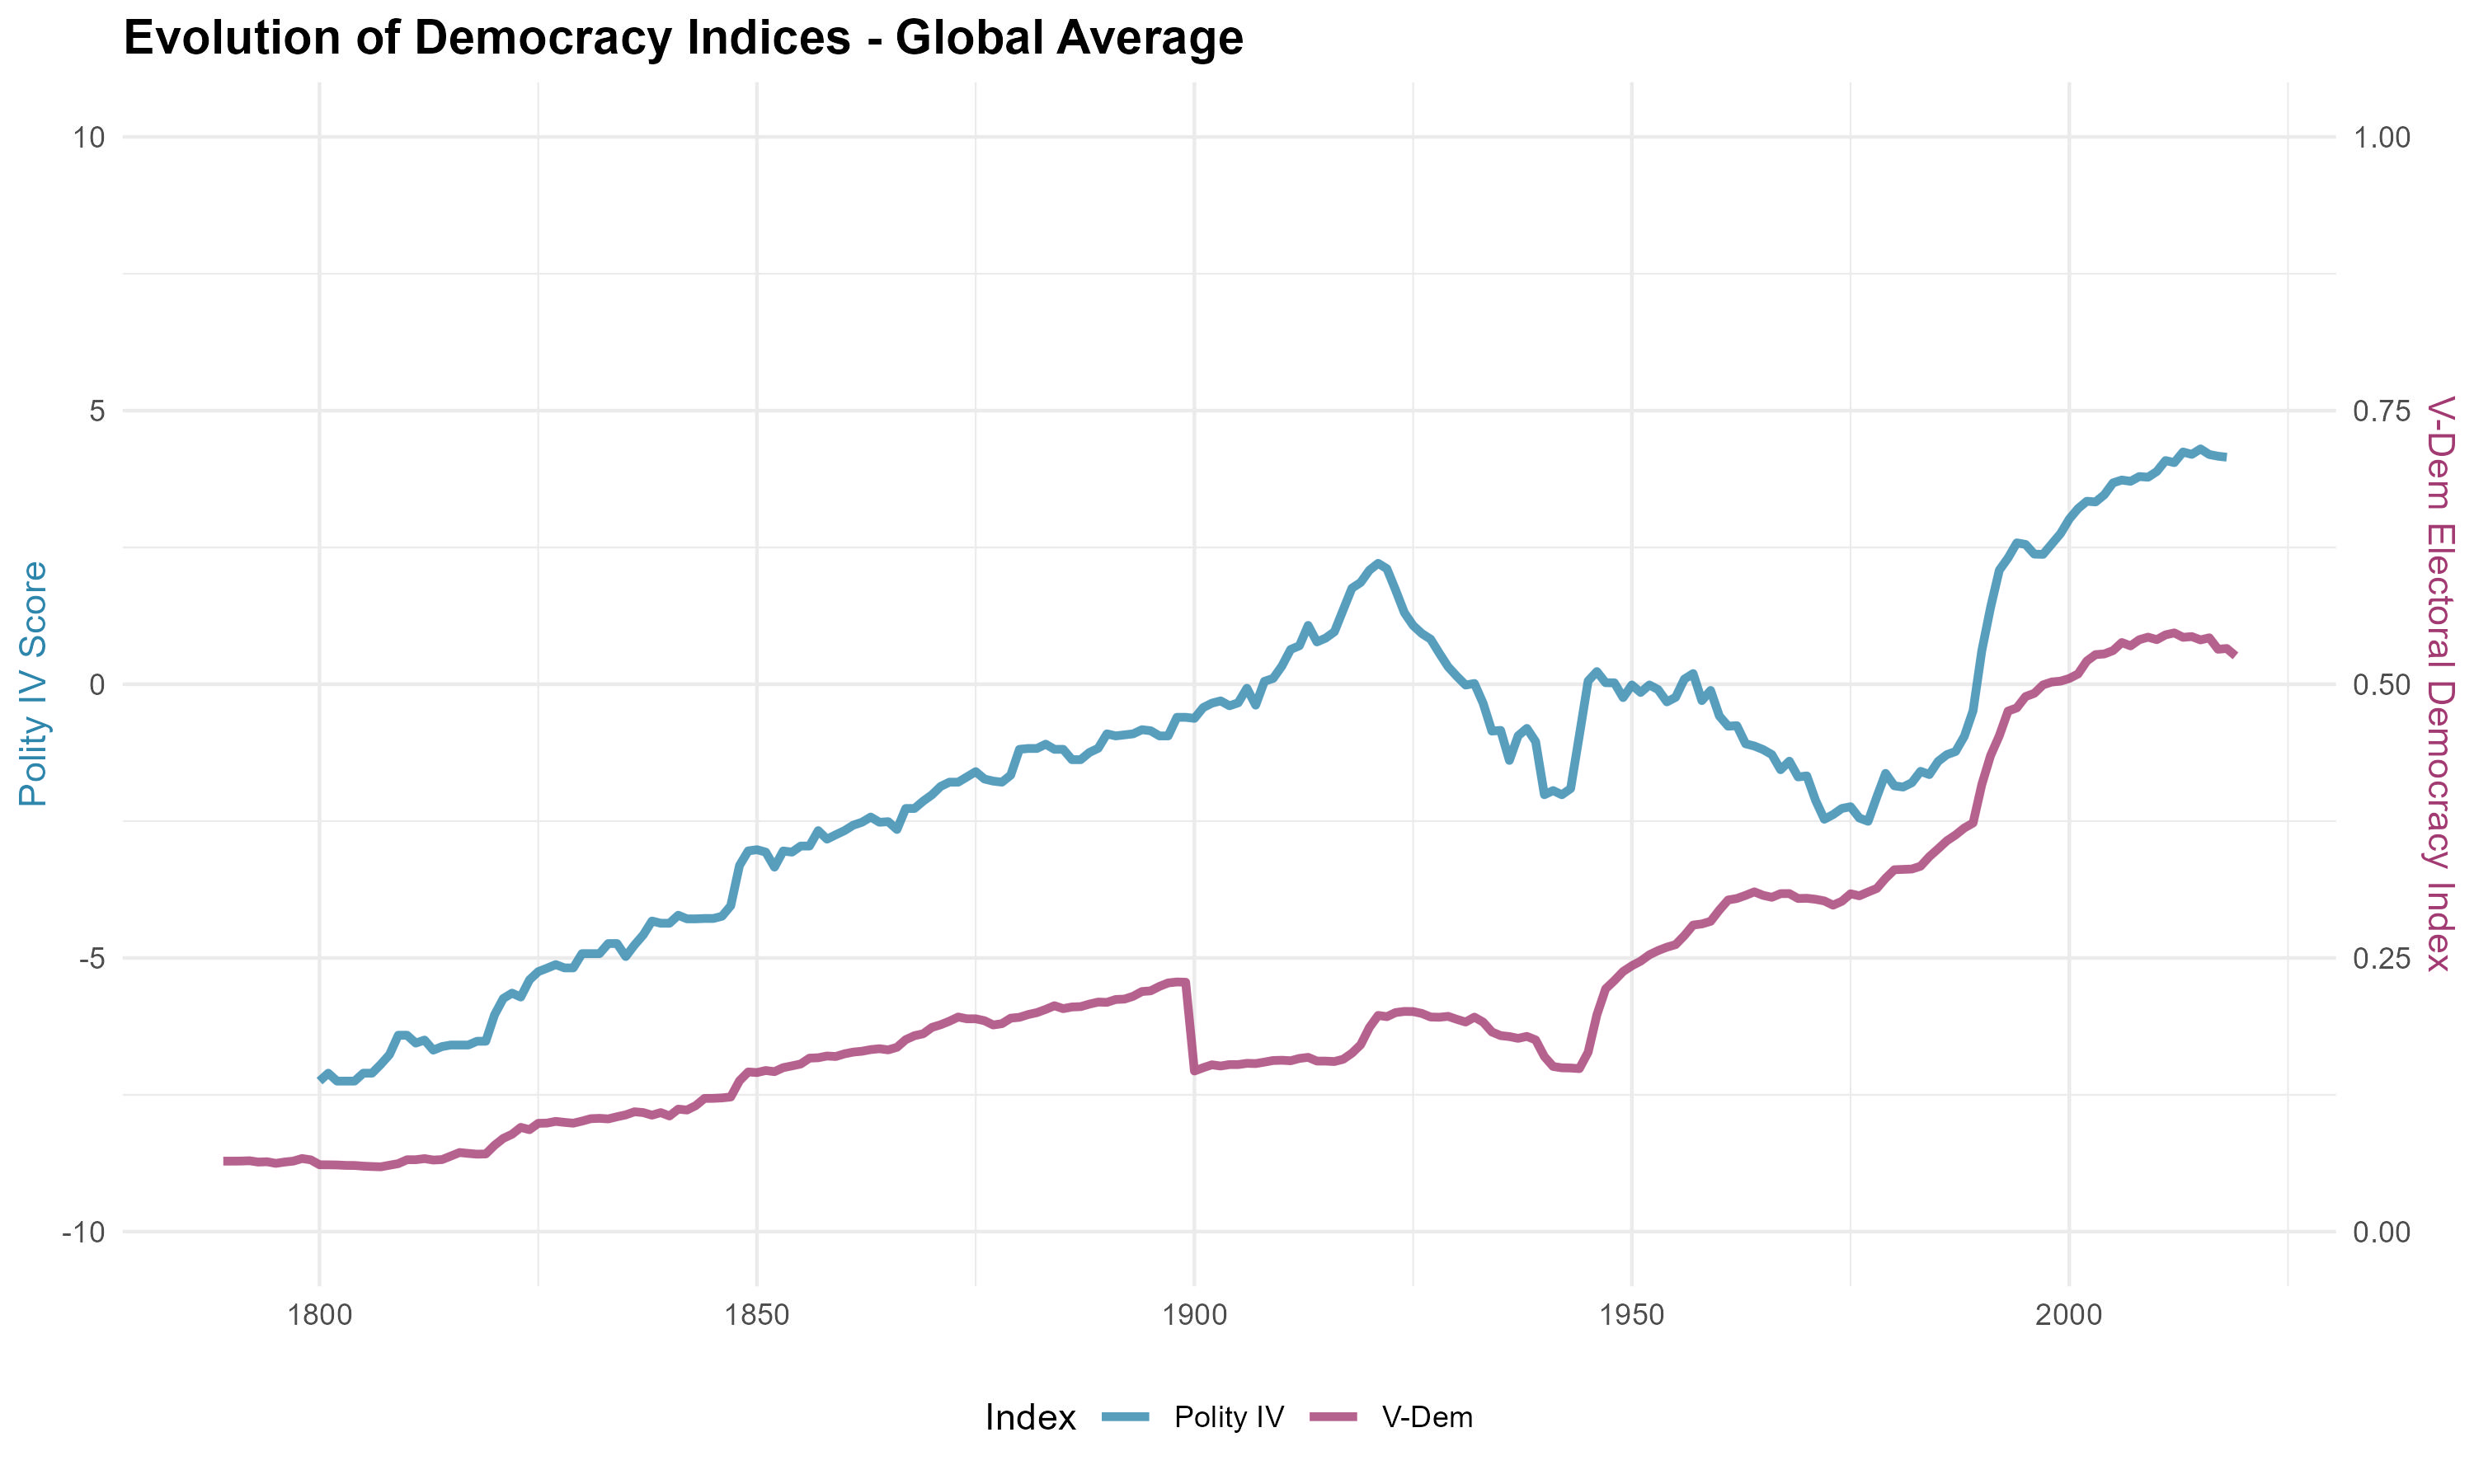
\includegraphics[scale=0.15]{C:/Users/Redha CHABA/Documents/wp_git/cdhm/plots/report/overall_trends.jpg}
        
    \vspace{1cm} 
    
    \caption{Regional Democracy Trends by Continent}
    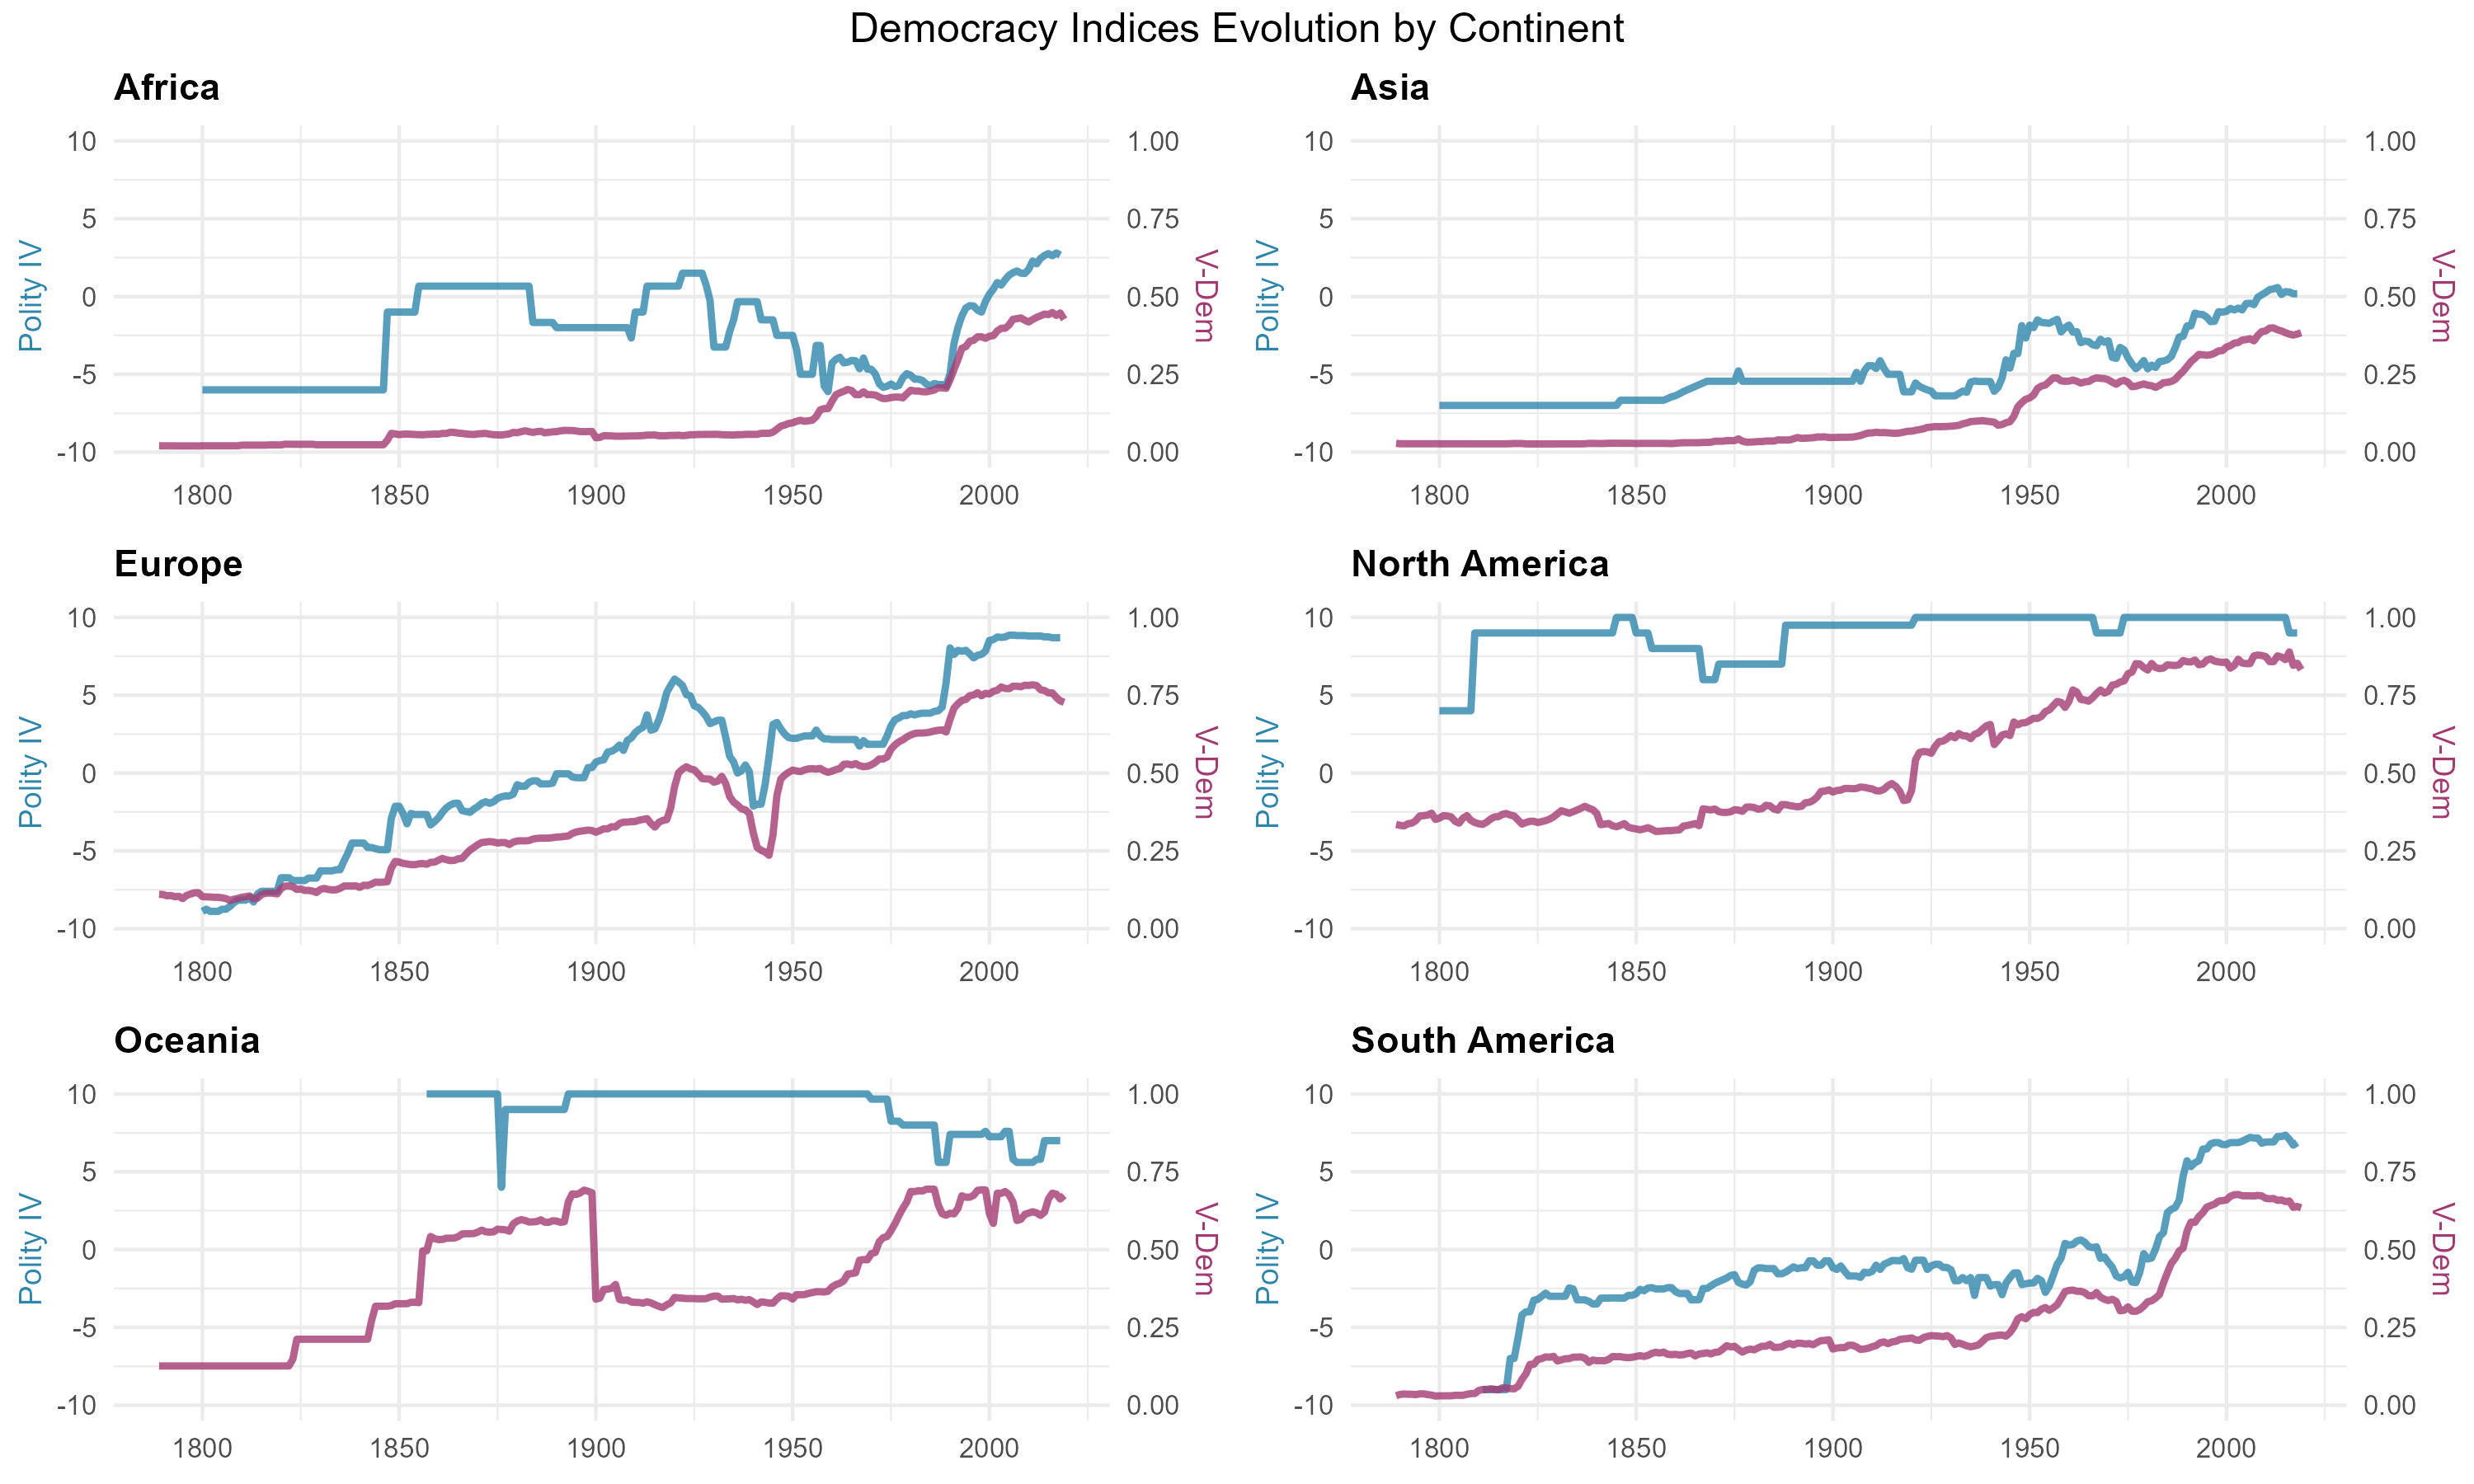
\includegraphics[scale=0.15]{C:/Users/Redha CHABA/Documents/wp_git/cdhm/plots/report/continent_trends.jpg}
    
    \end{center}
\end{figure}

\begin{figure}[H]
    \begin{center}
    \caption{Democracy and Youth Demographics - Global Relationship}
    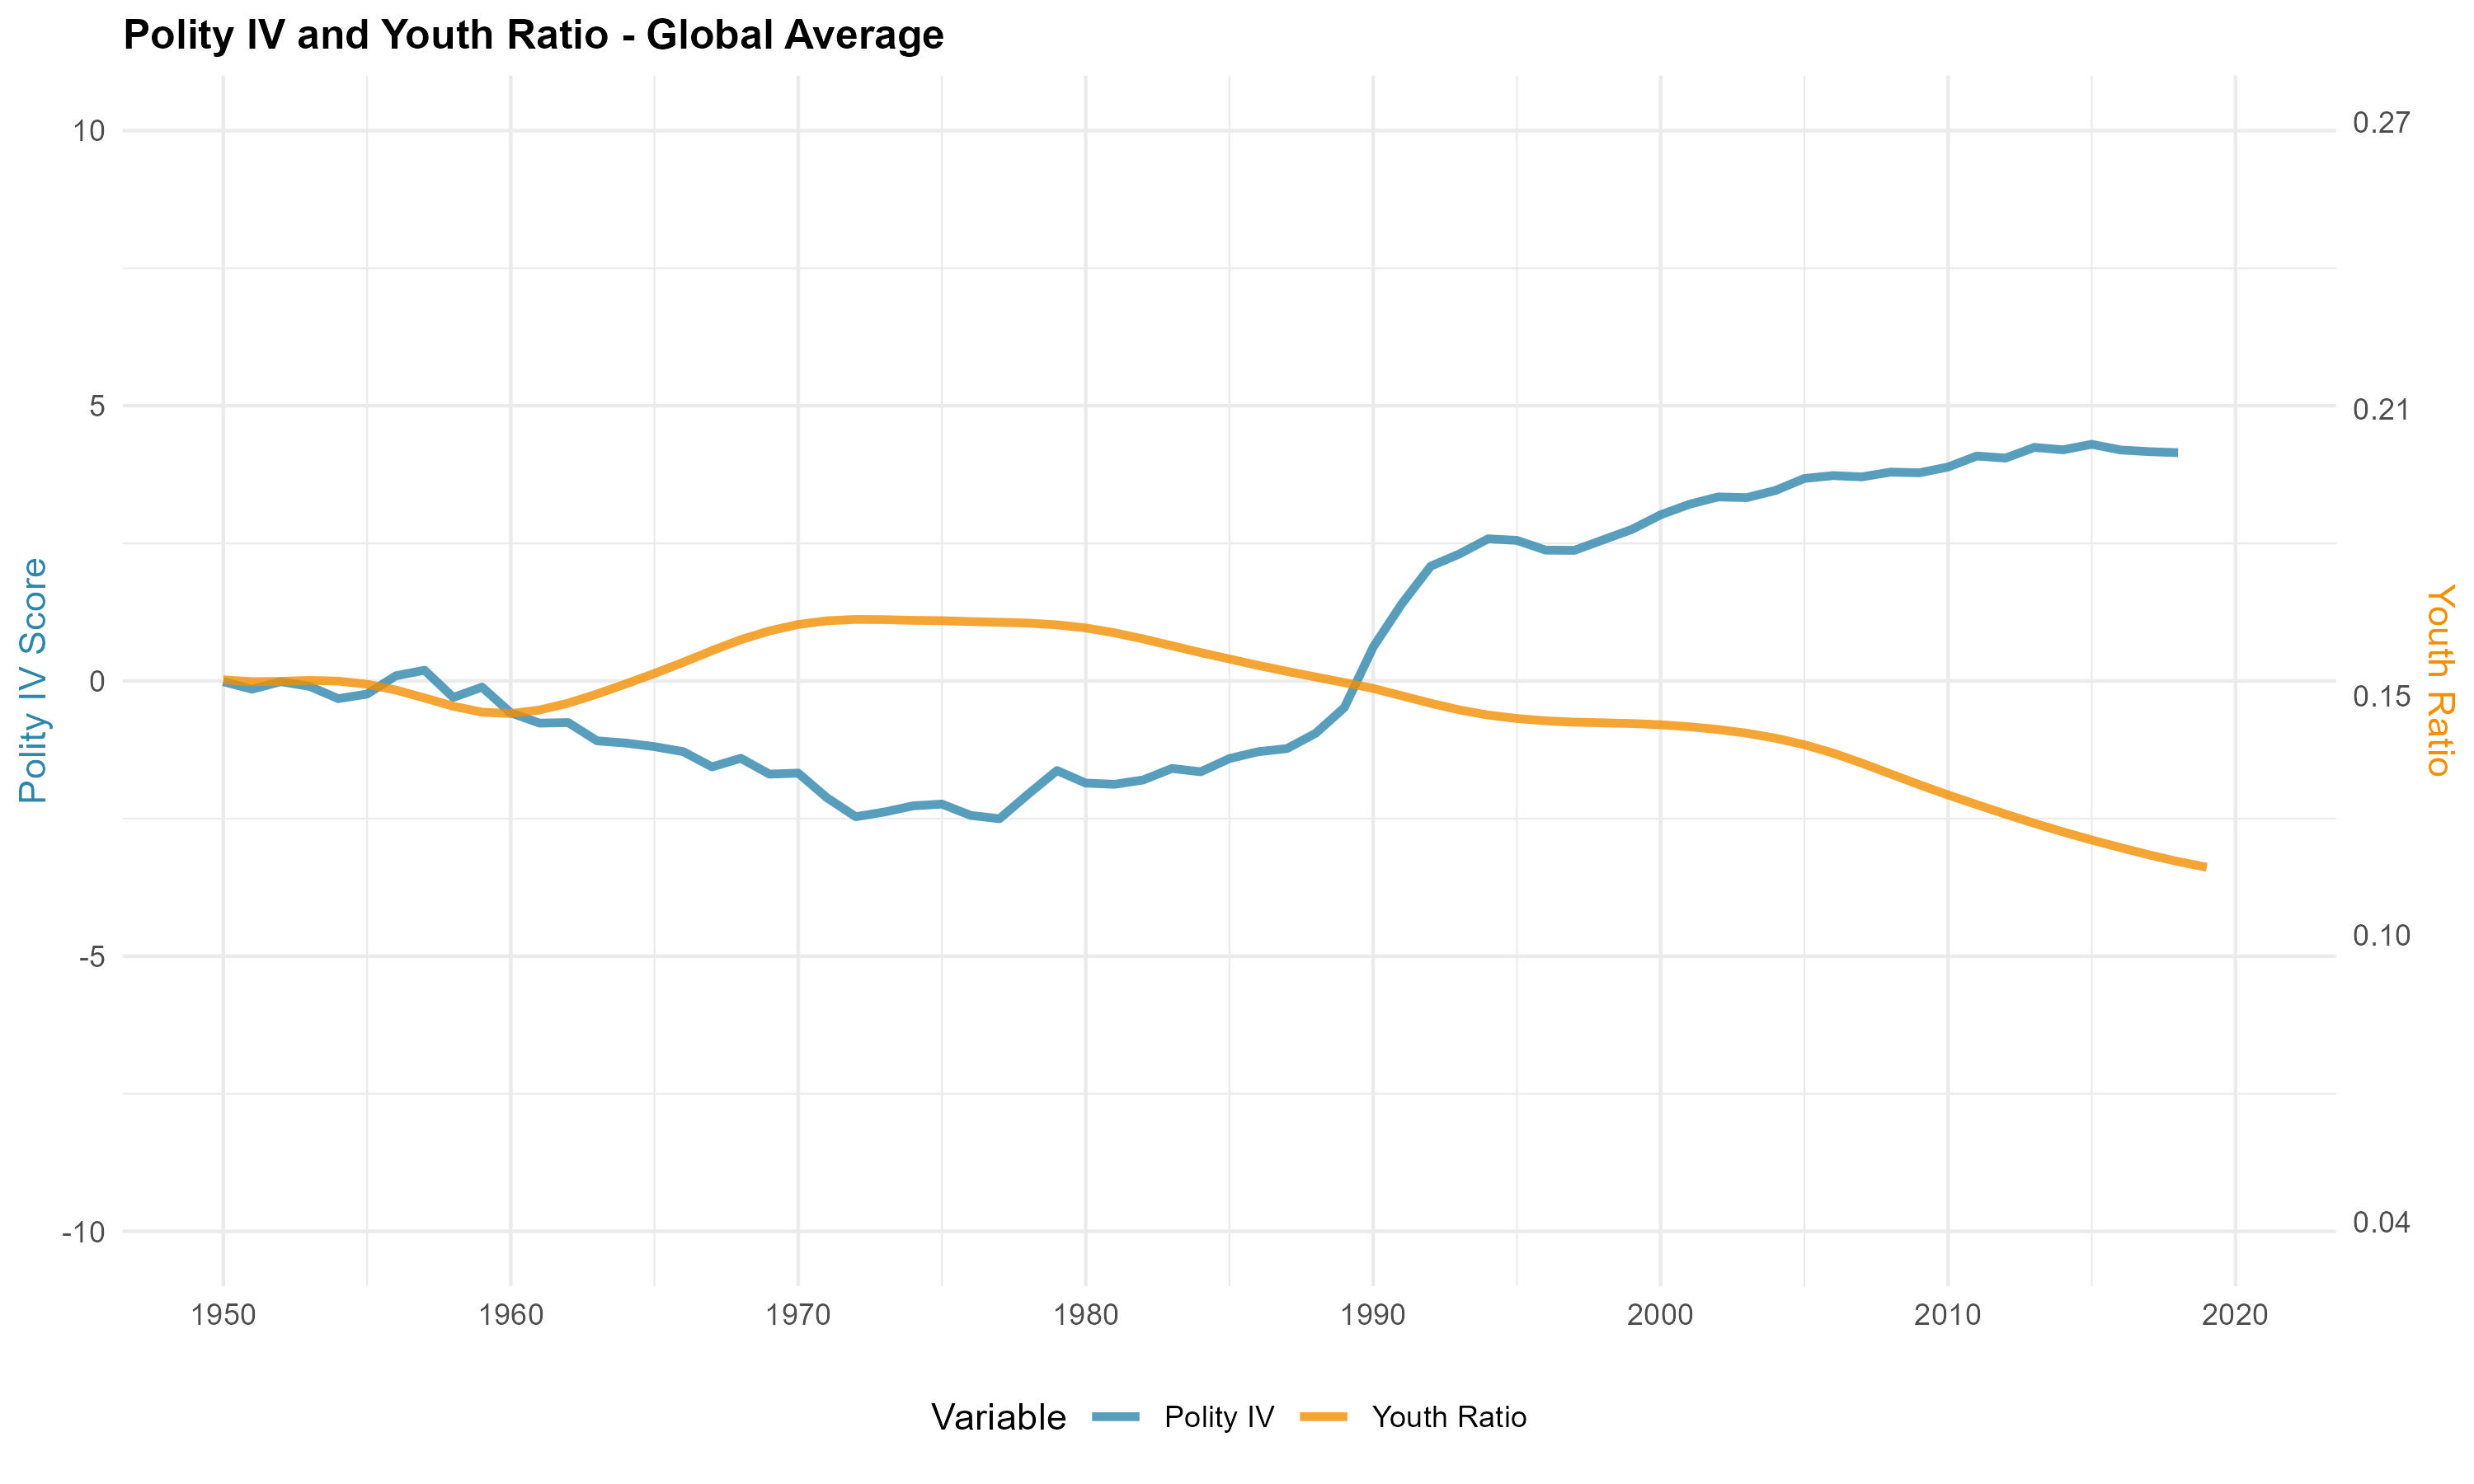
\includegraphics[scale=0.15]{C:/Users/Redha CHABA/Documents/wp_git/cdhm/plots/report/overall_youth_polity.jpg}
    
    \vspace{1cm} 
    
    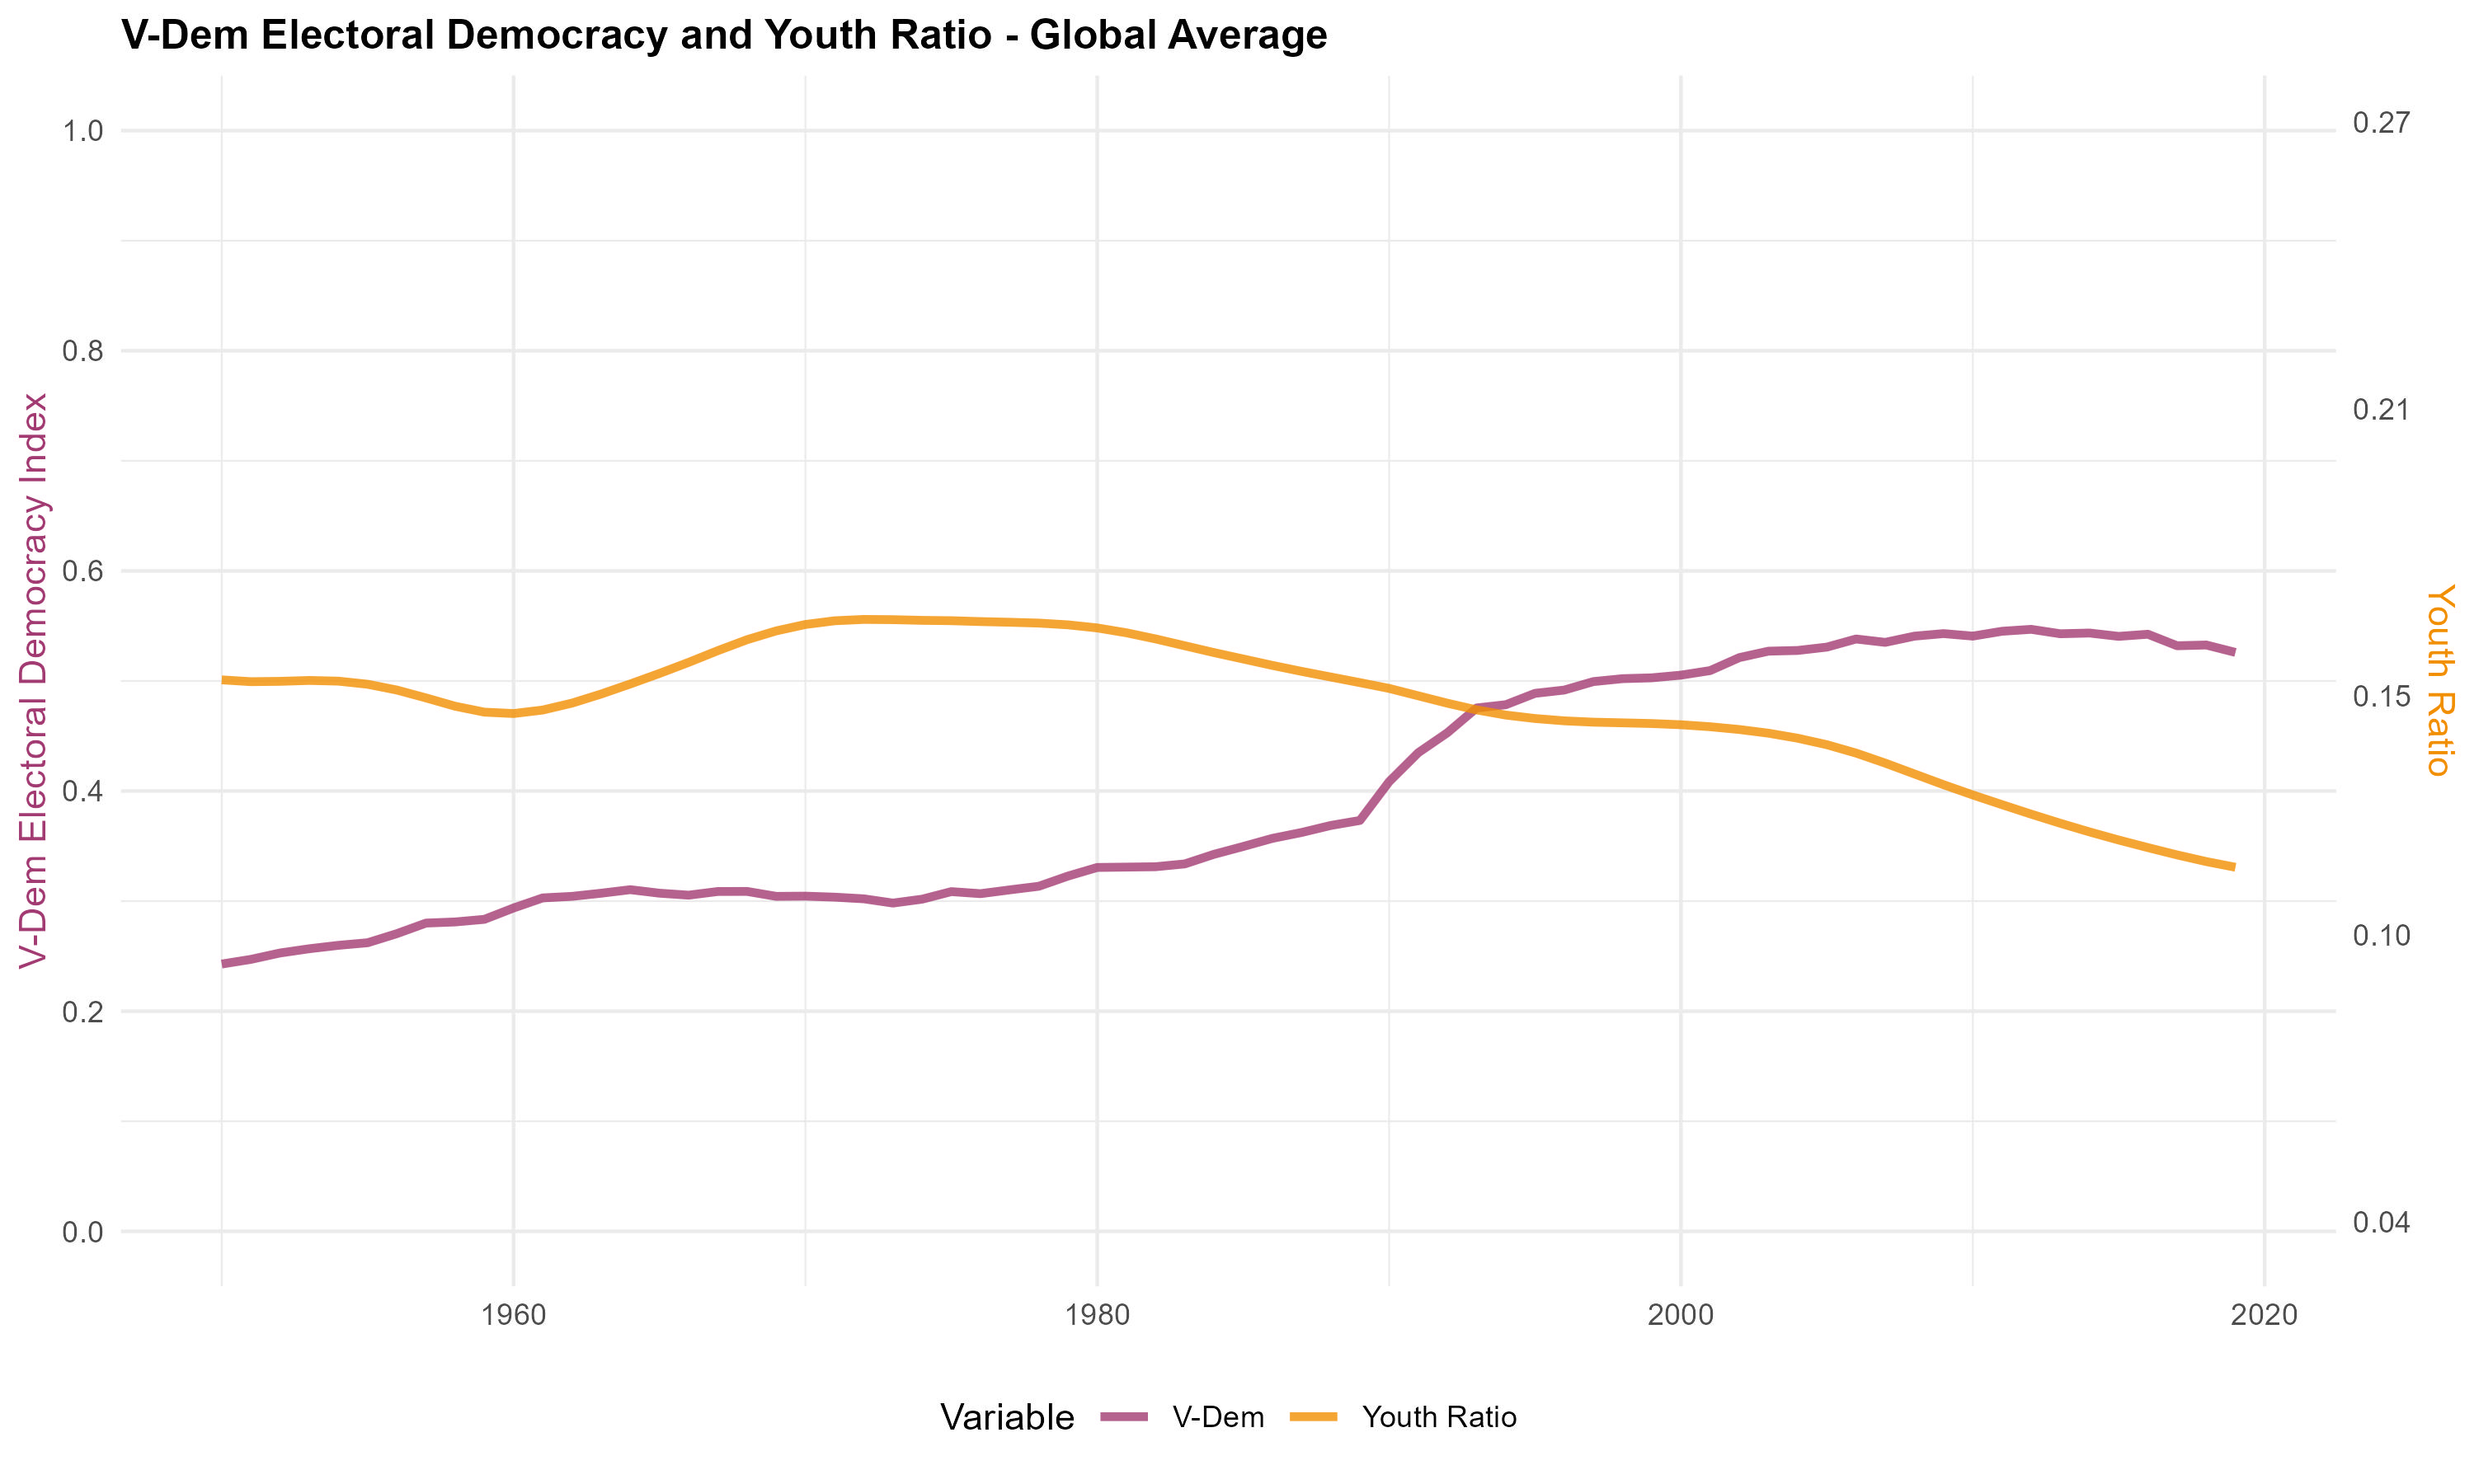
\includegraphics[scale=0.15]{C:/Users/Redha CHABA/Documents/wp_git/cdhm/plots/report/overall_youth_vdem.jpg}
    \end{center}
\end{figure}

\begin{figure}[H]
    \begin{center}
    \caption{Regional Patterns: Democracy-Youth Relationship by Continent}
    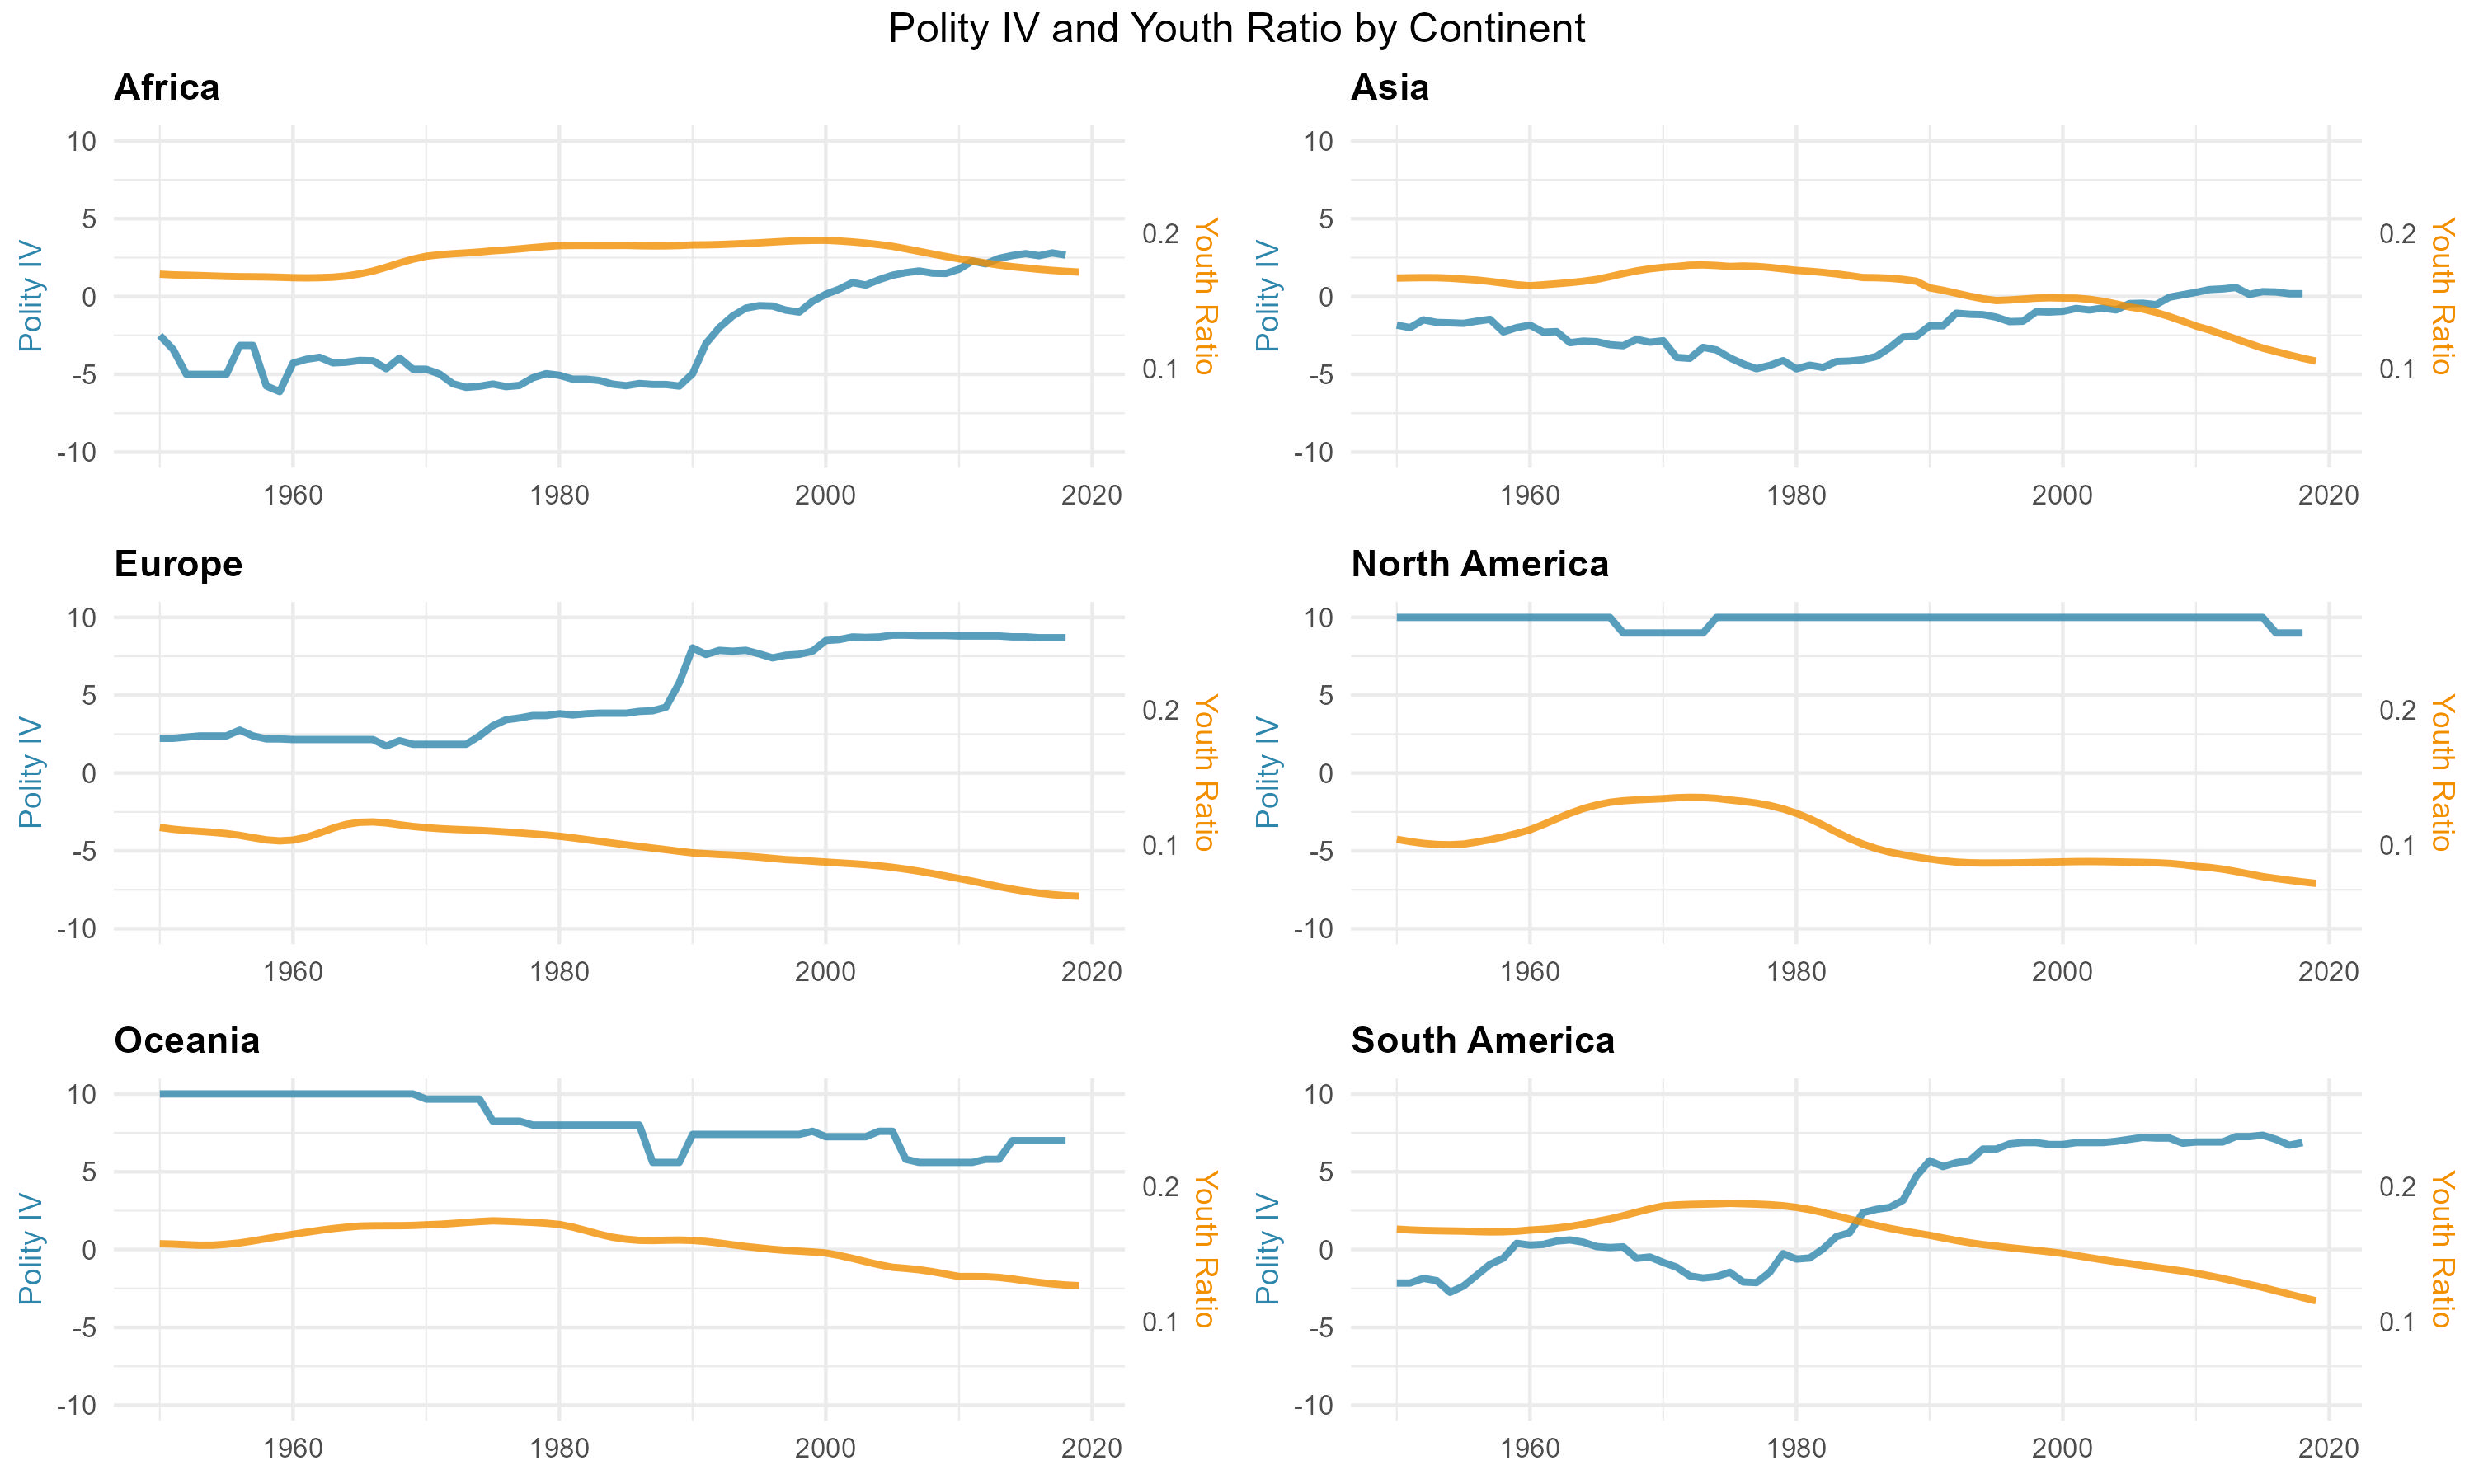
\includegraphics[scale=0.15]{C:/Users/Redha CHABA/Documents/wp_git/cdhm/plots/report/continent_youth_polity.jpg}
        
    \vspace{1cm}

    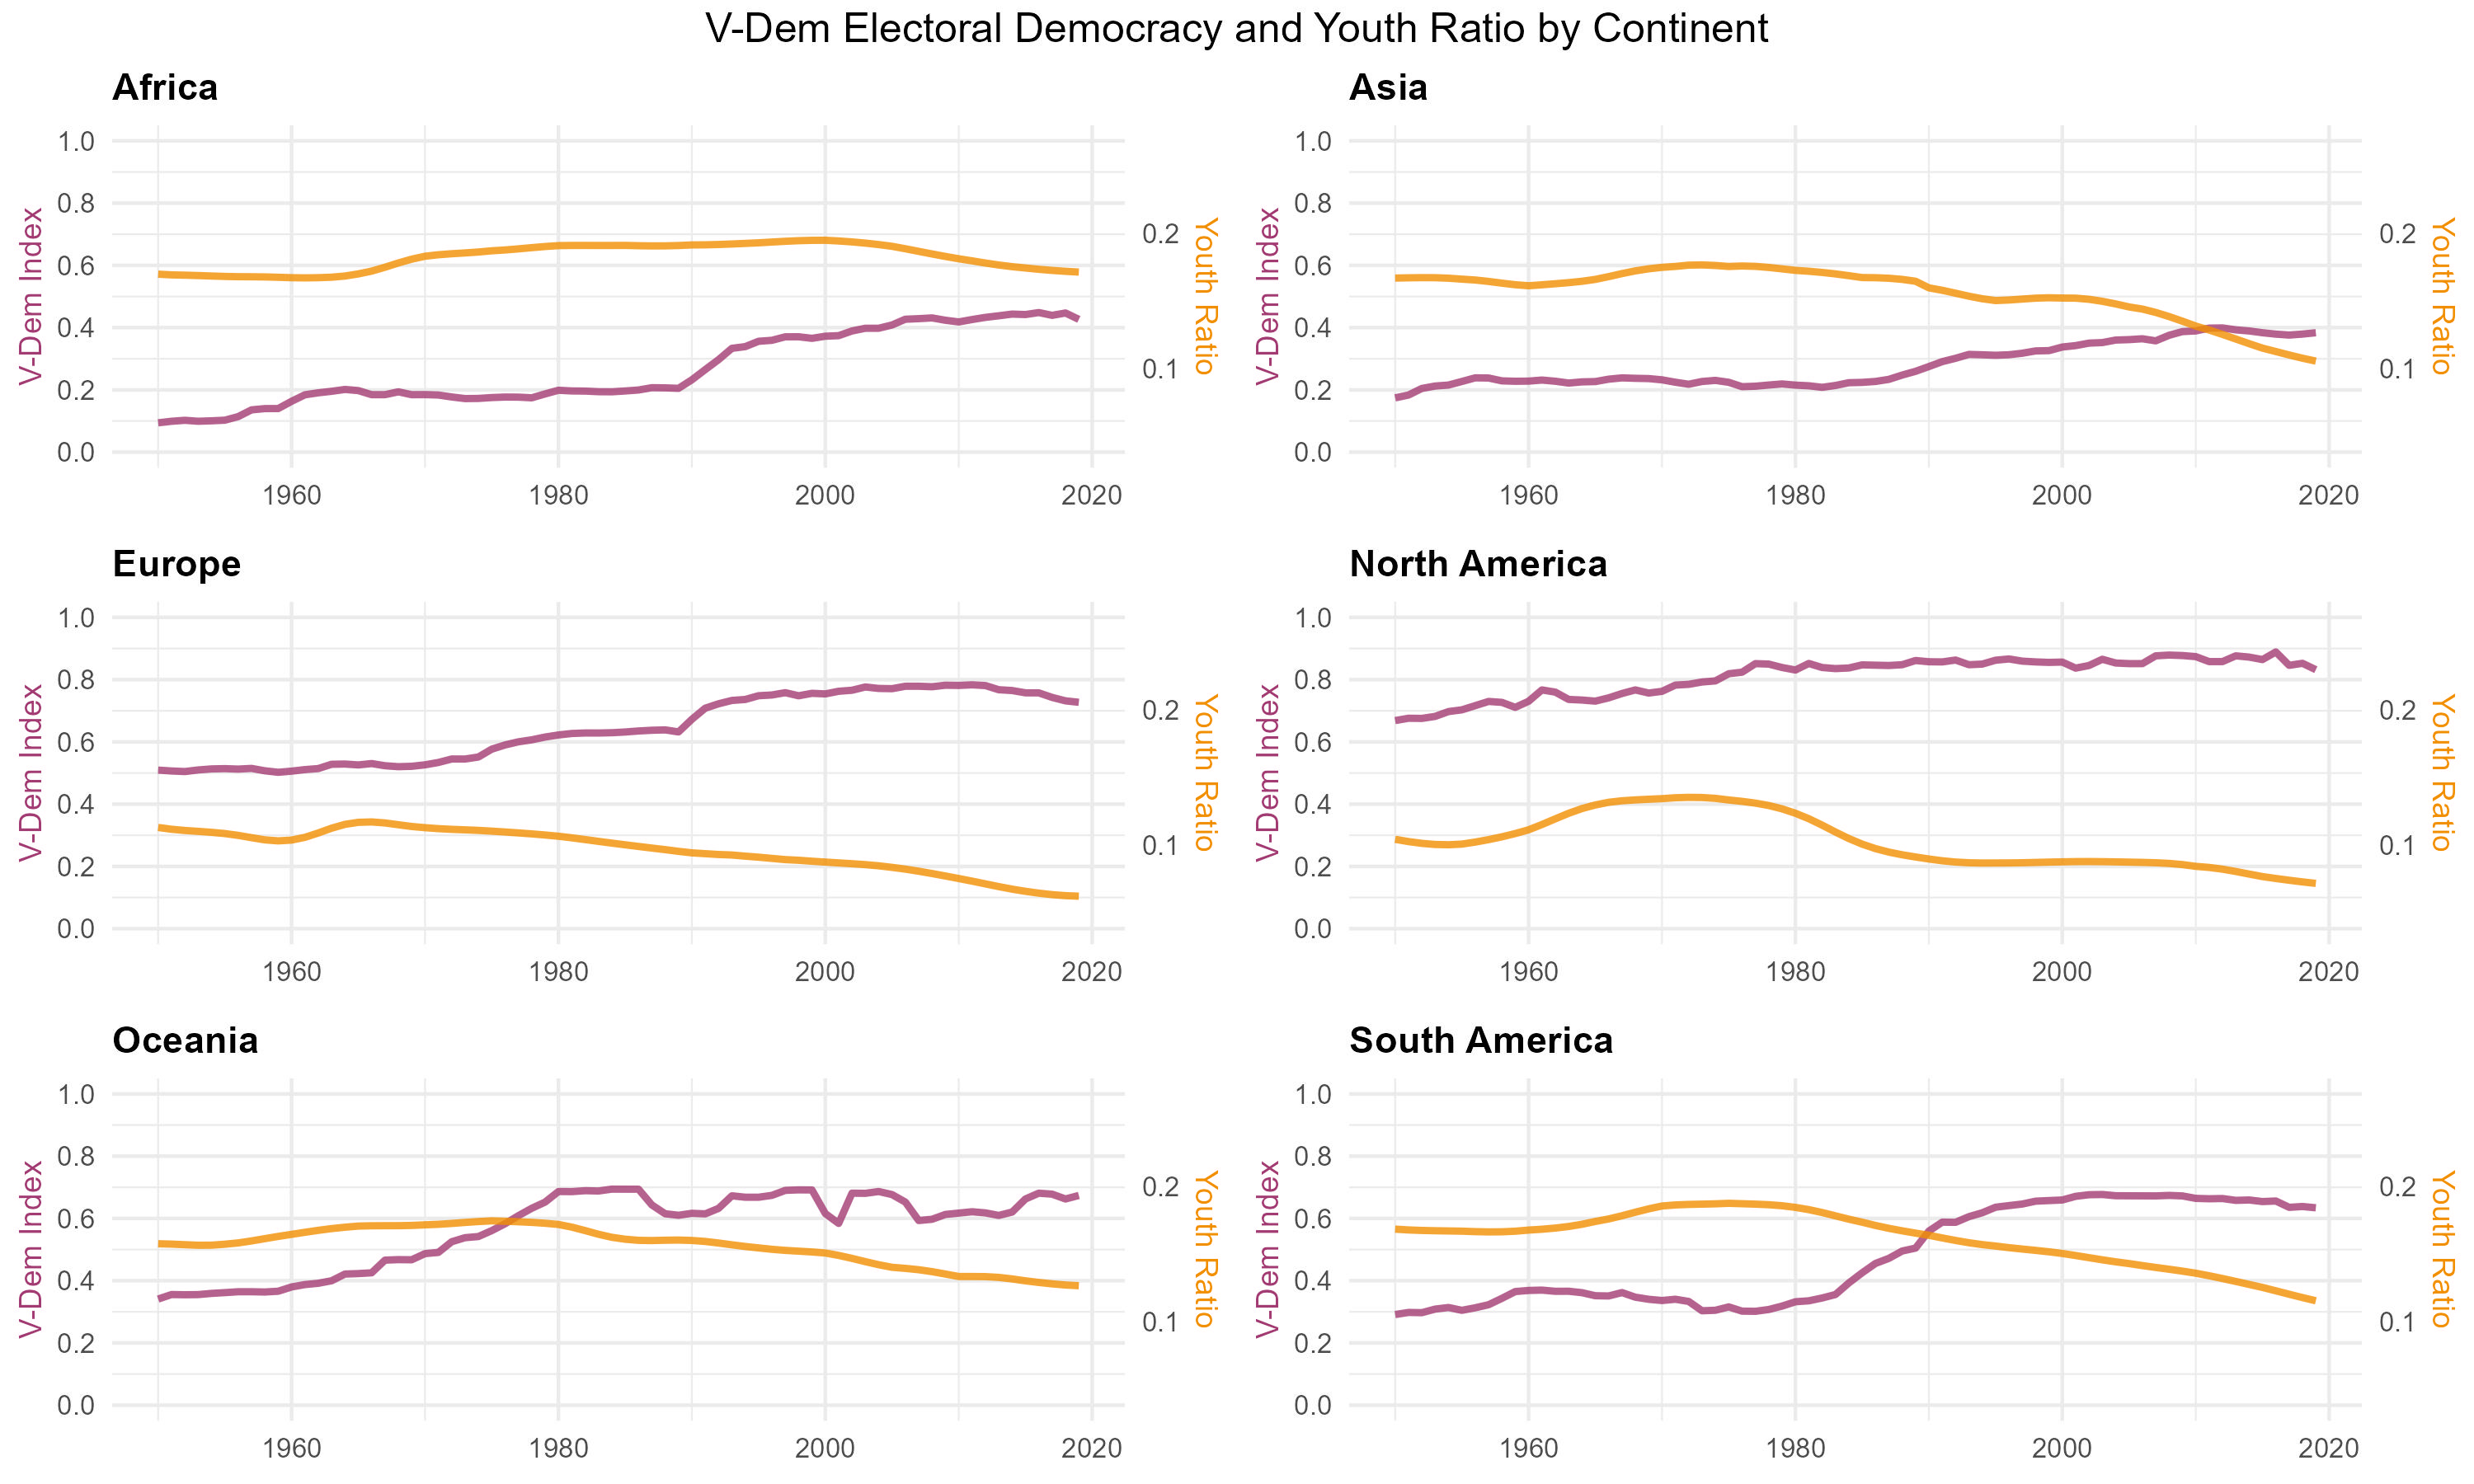
\includegraphics[scale=0.15]{C:/Users/Redha CHABA/Documents/wp_git/cdhm/plots/report/continent_youth_vdem.jpg}
    \end{center}
\end{figure}

\begin{figure}[H]
    \begin{center}
    \caption{Distribution of Democracy Scores}
    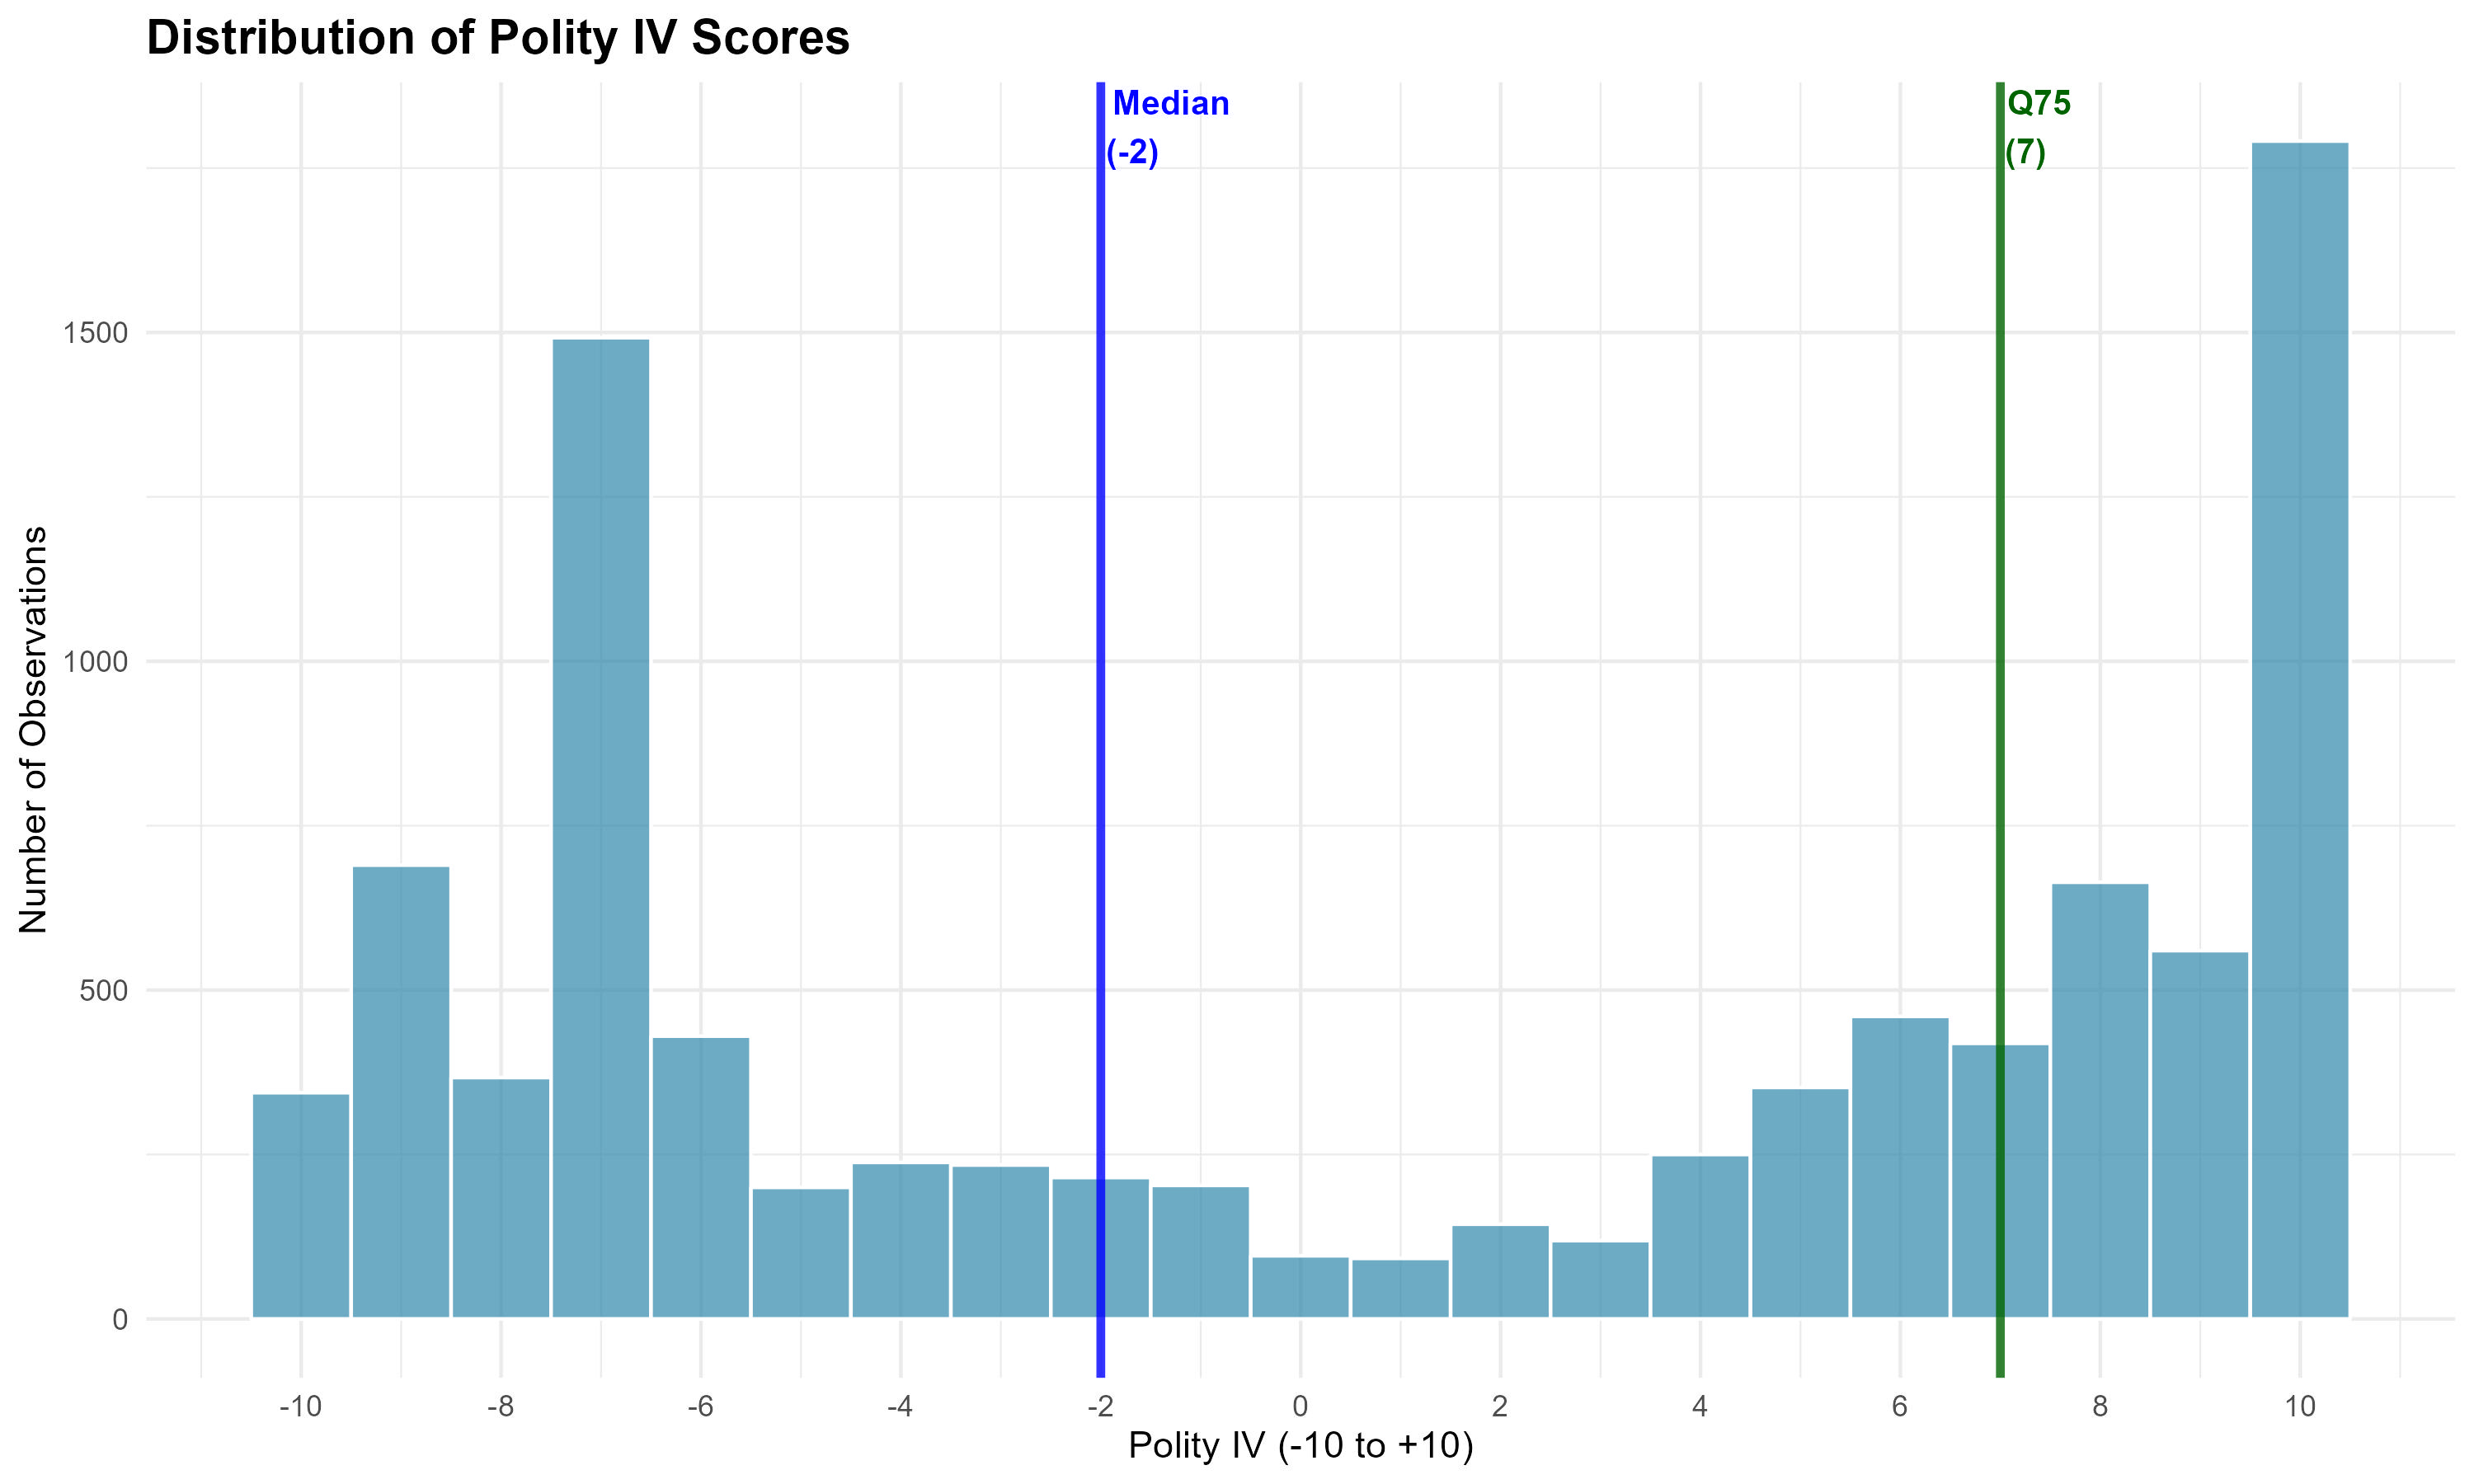
\includegraphics[scale=0.15]{C:/Users/Redha CHABA/Documents/wp_git/cdhm/plots/report/hist_polity.jpg}
    
    \vspace{1cm}

    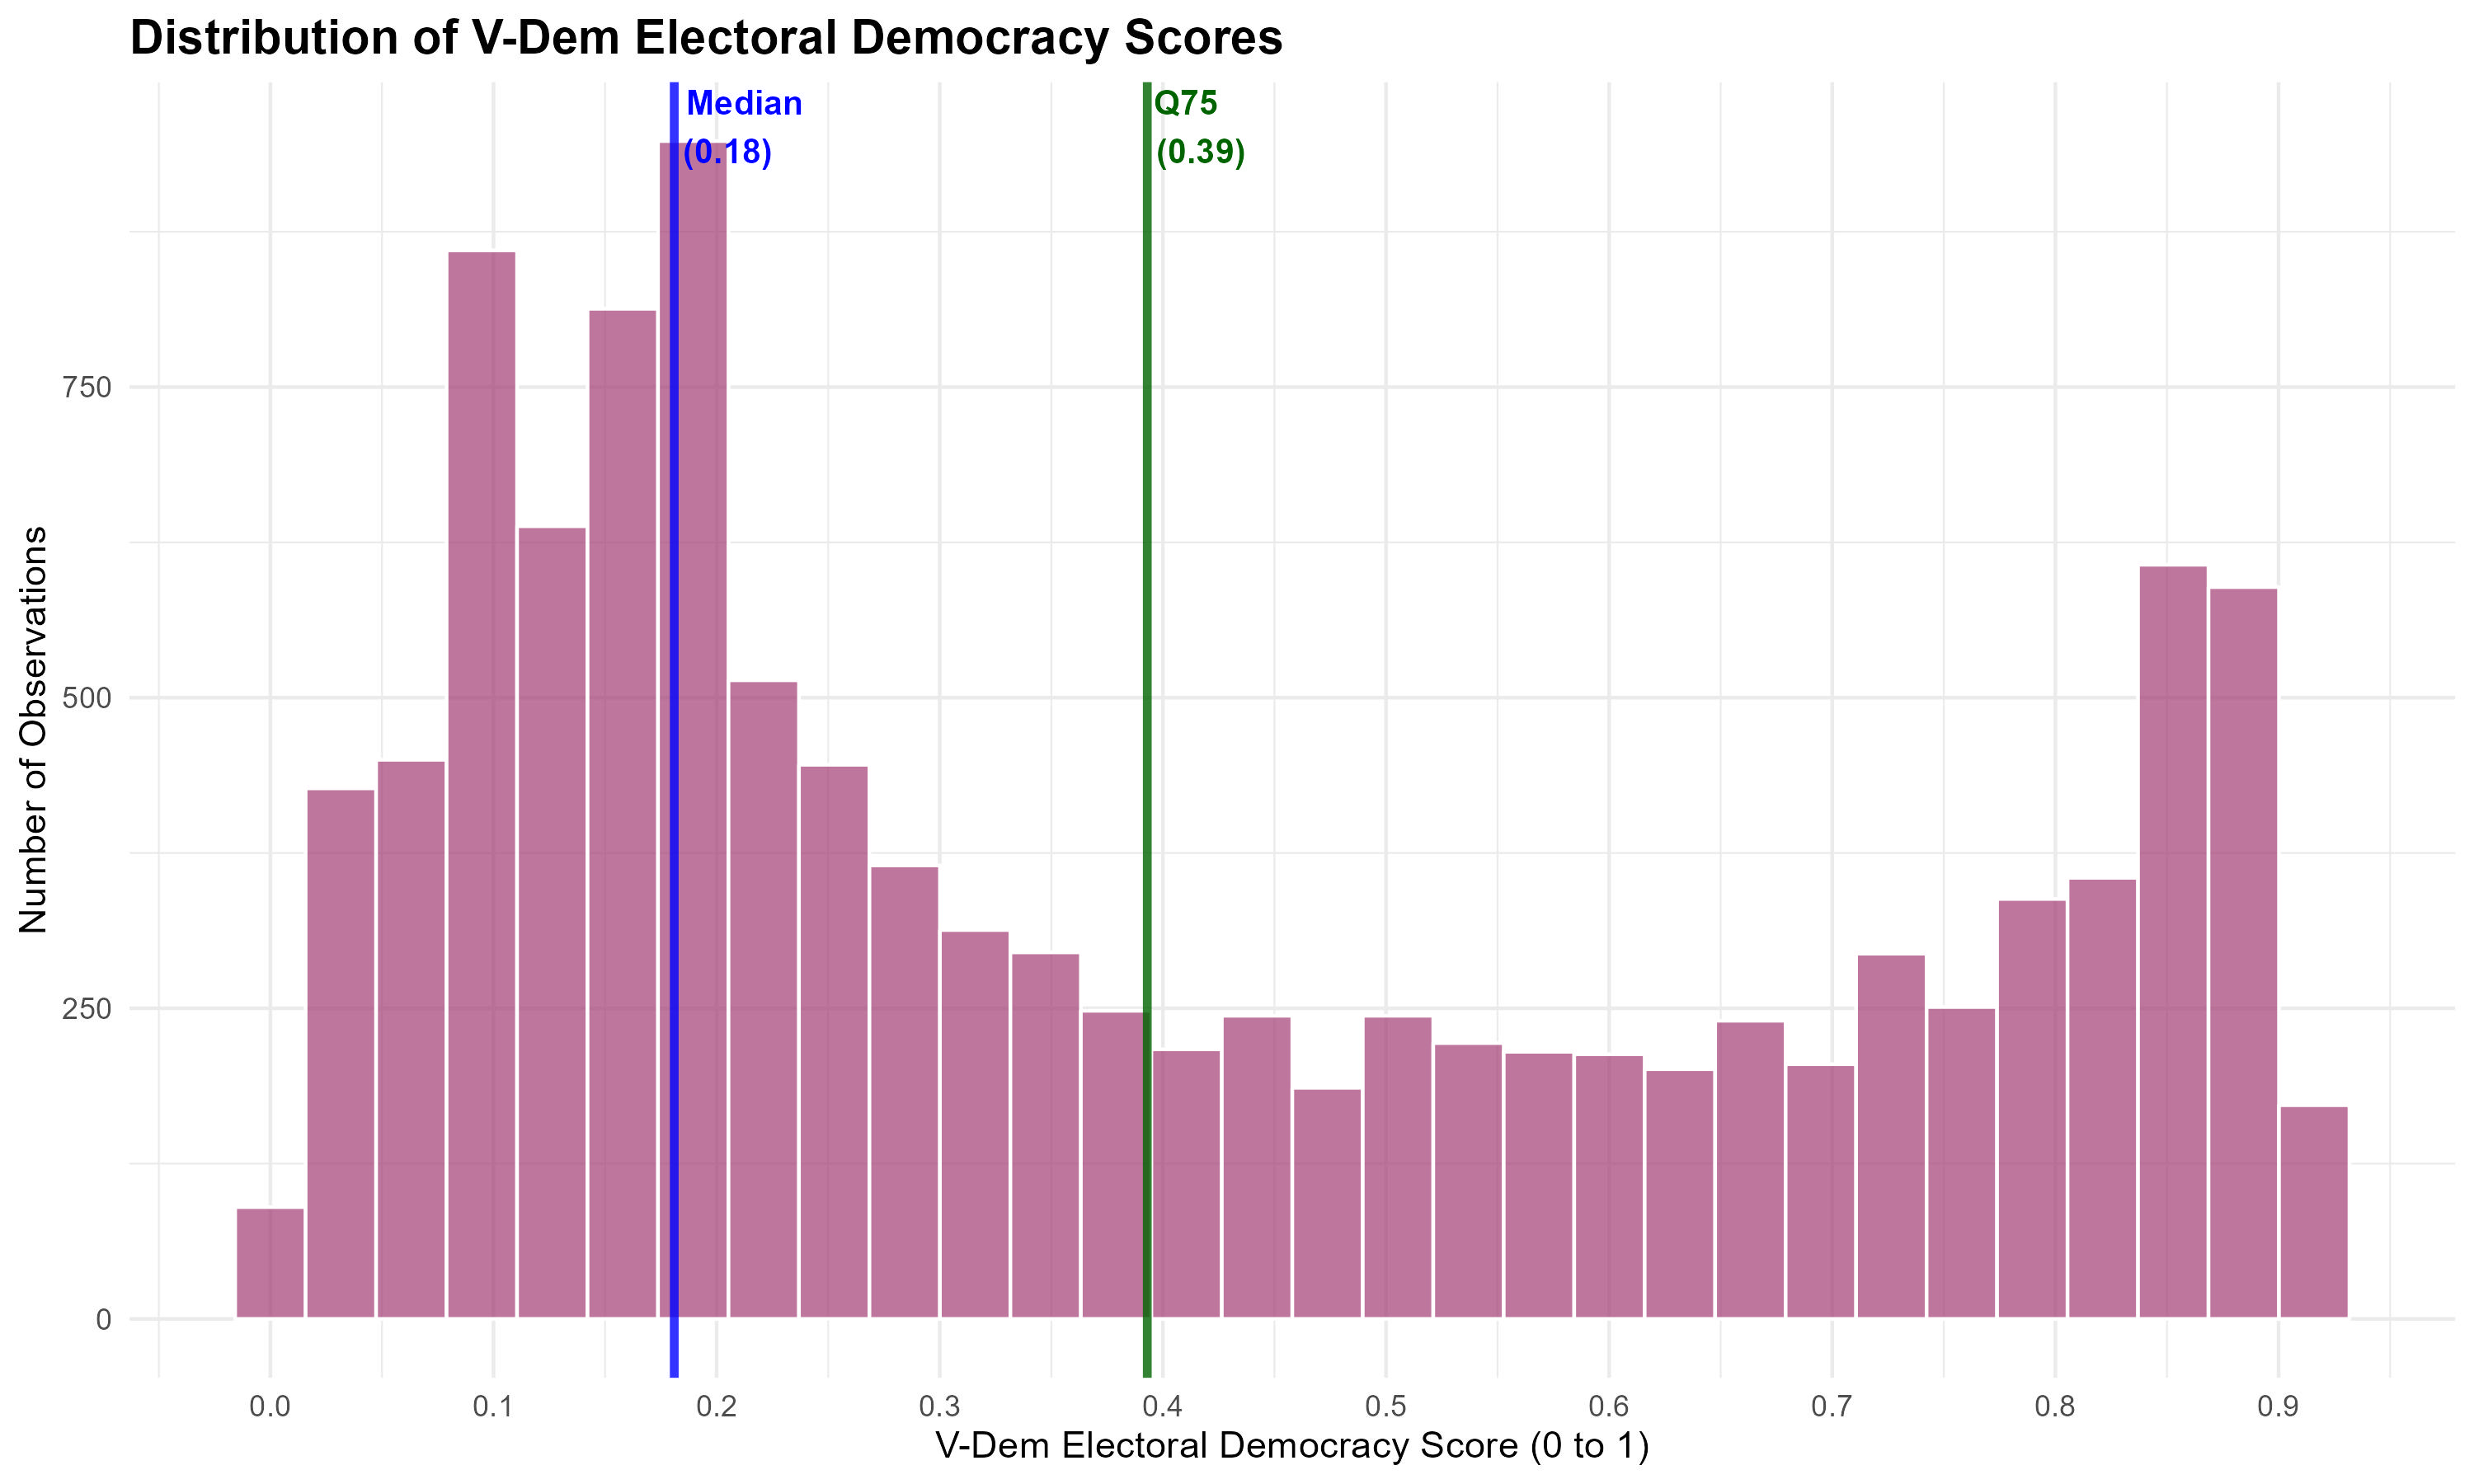
\includegraphics[scale=0.15]{C:/Users/Redha CHABA/Documents/wp_git/cdhm/plots/report/hist_vdem.jpg}
    \end{center}
\end{figure}

\begin{figure}[H]
    \begin{center}
    \caption{Regime Type Classifications}
    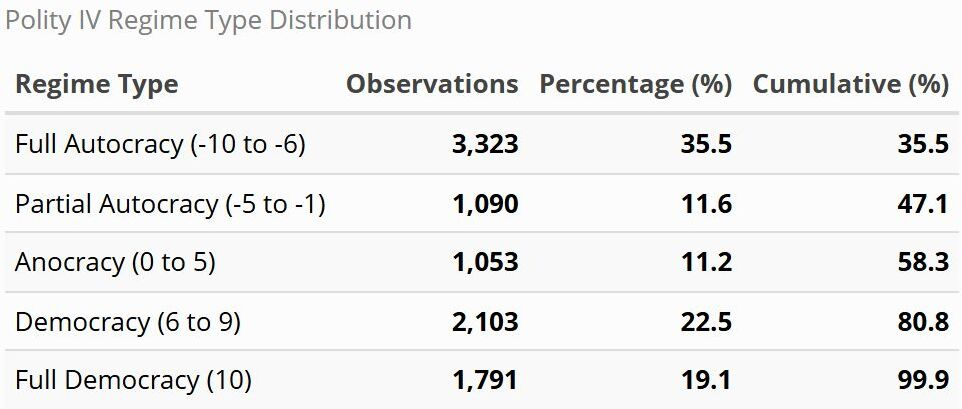
\includegraphics[scale=1.5]{C:/Users/Redha CHABA/Documents/wp_git/cdhm/plots/report/regime_table_polity.jpg}
        
    \vspace{1cm}

    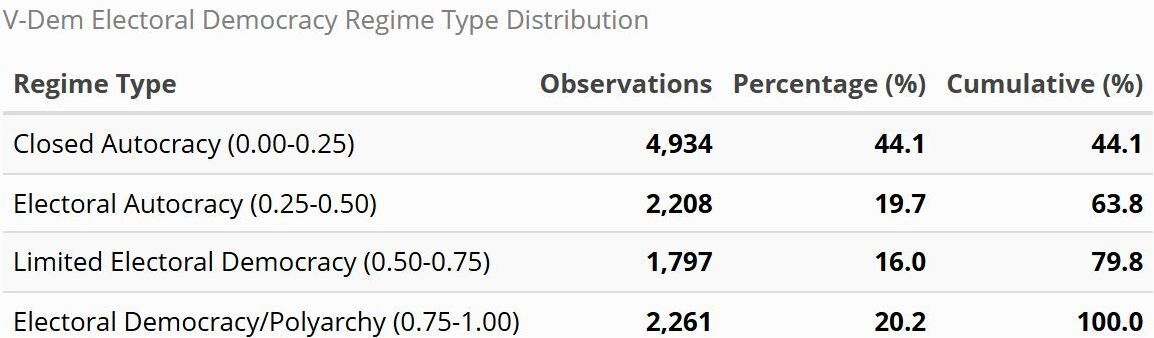
\includegraphics[scale=1.5]{C:/Users/Redha CHABA/Documents/wp_git/cdhm/plots/report/regime_table_vdem.jpg}
    \end{center}
\end{figure}

\begin{figure}[H]
    \begin{center}
    \caption{Cumulative Distribution of Democracy Scores}
    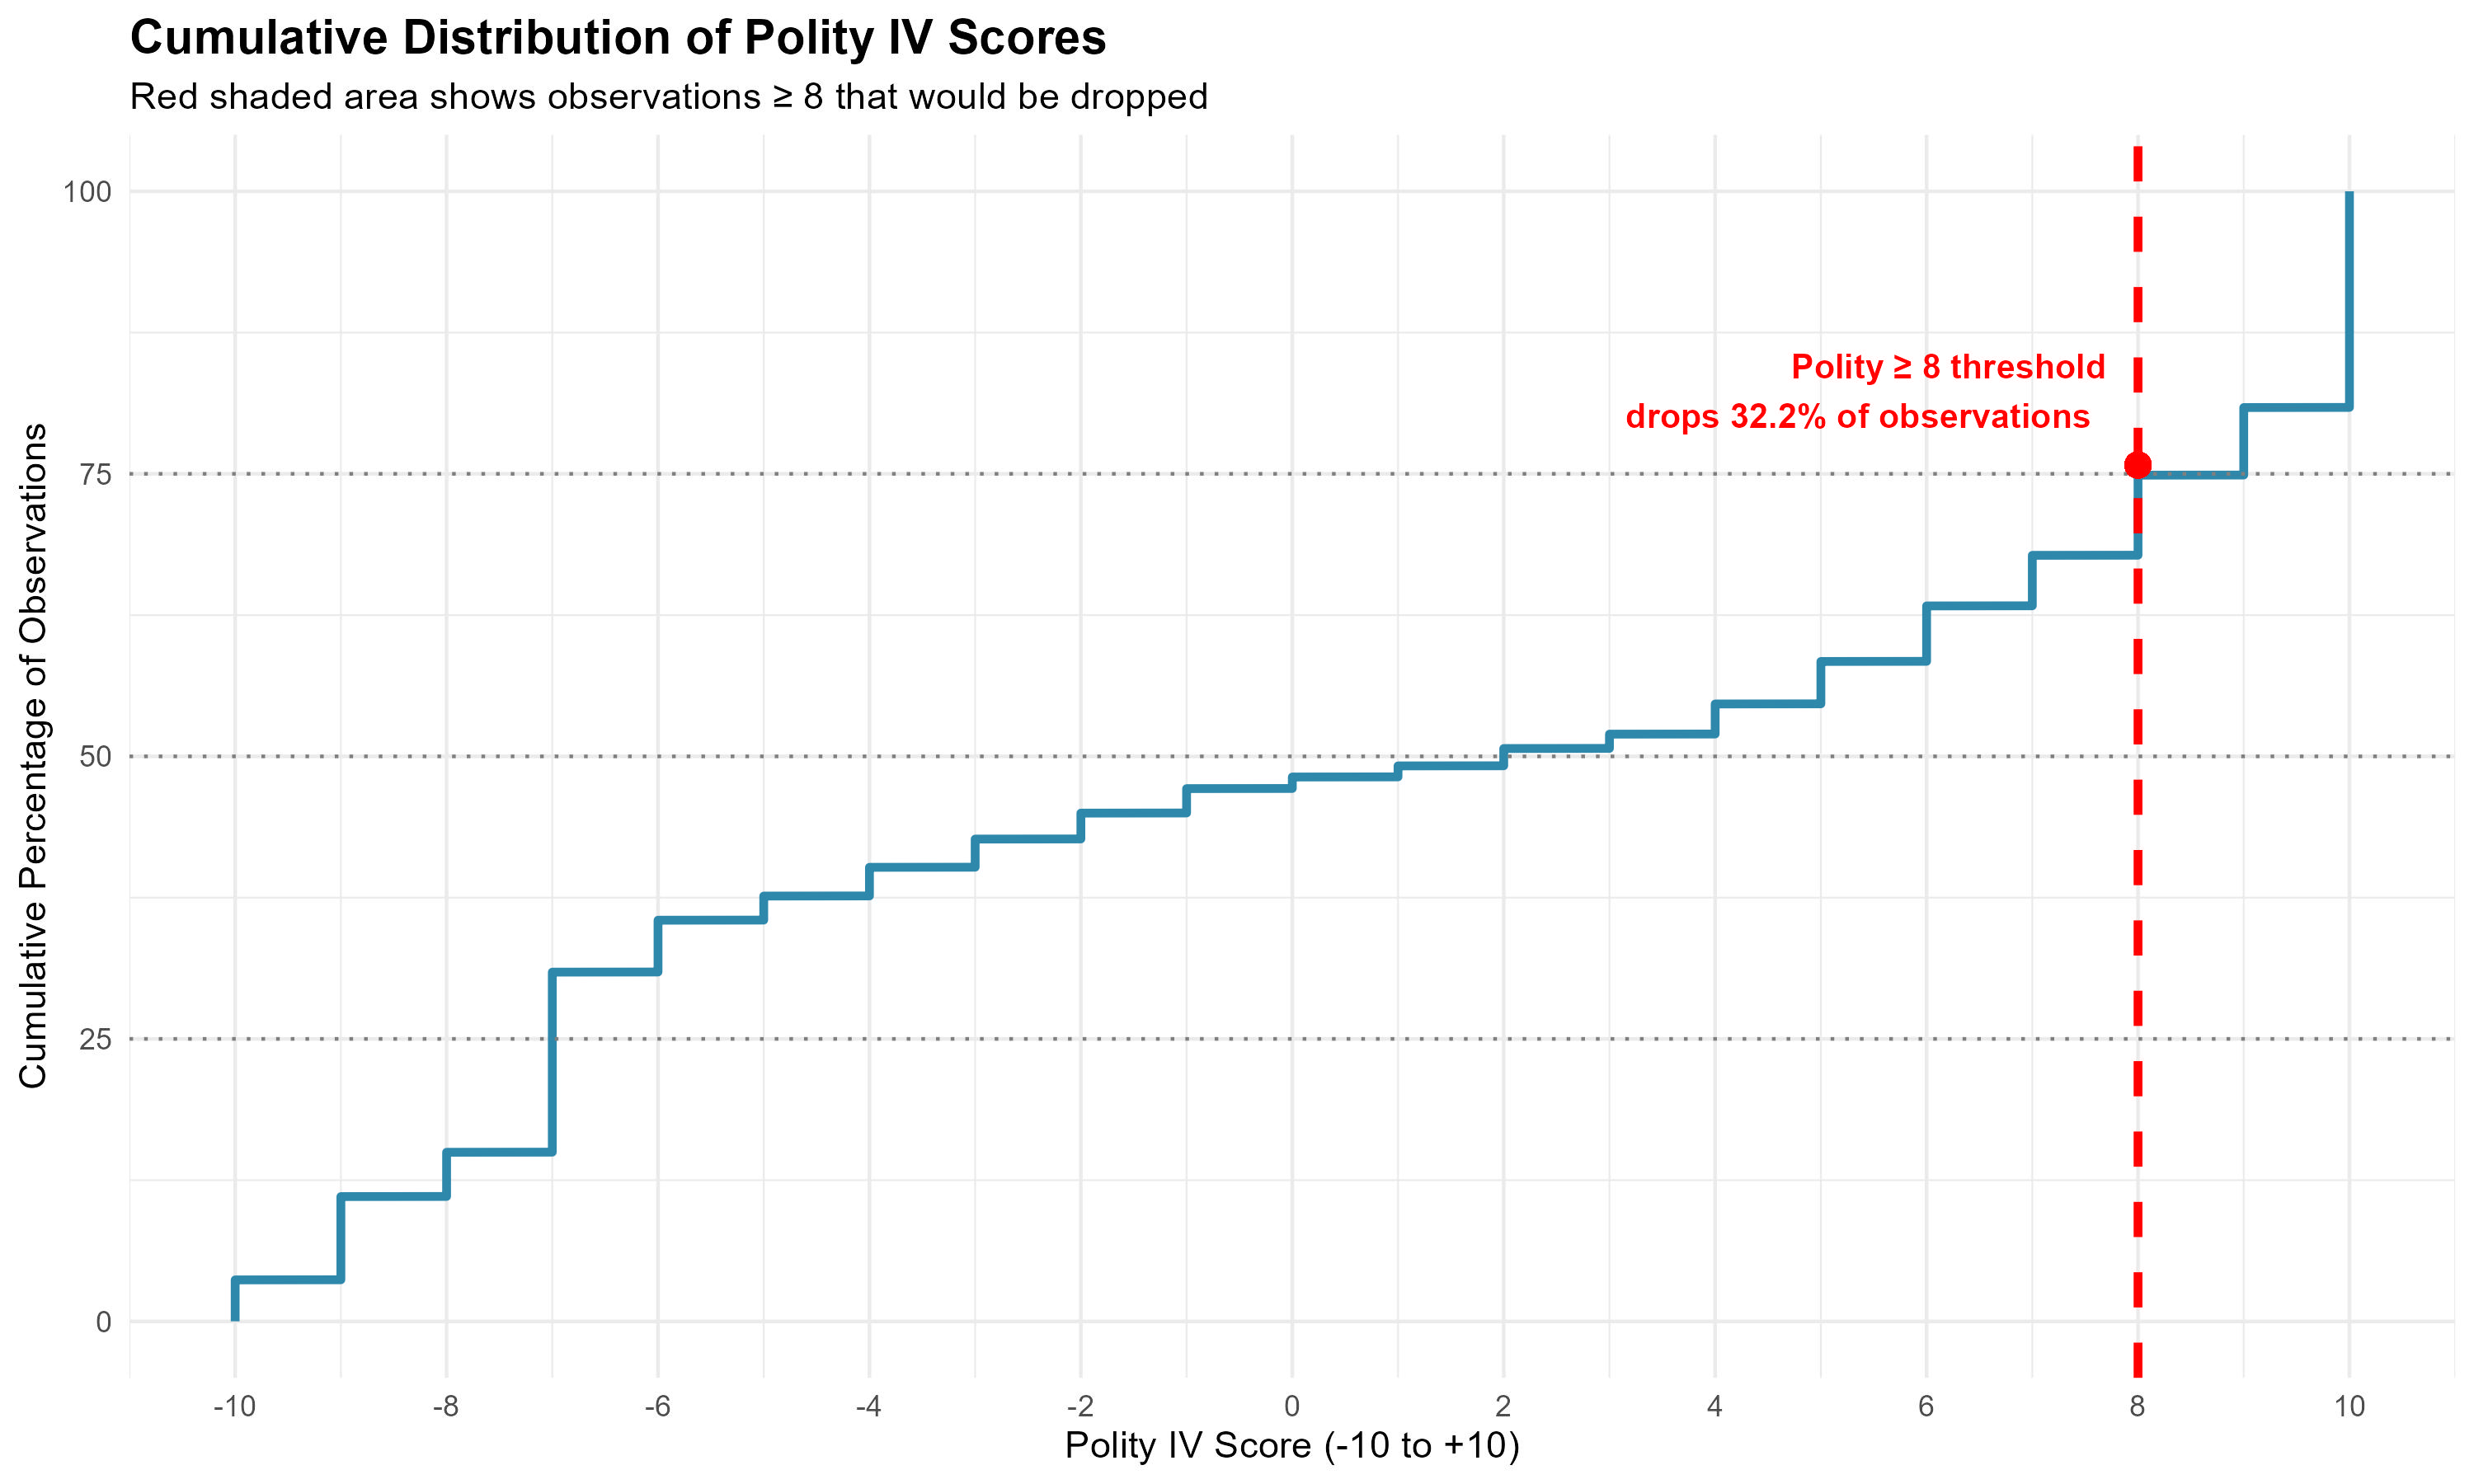
\includegraphics[scale=0.15]{C:/Users/Redha CHABA/Documents/wp_git/cdhm/plots/report/cumul_polity.jpg}
        
    \vspace{1cm}

    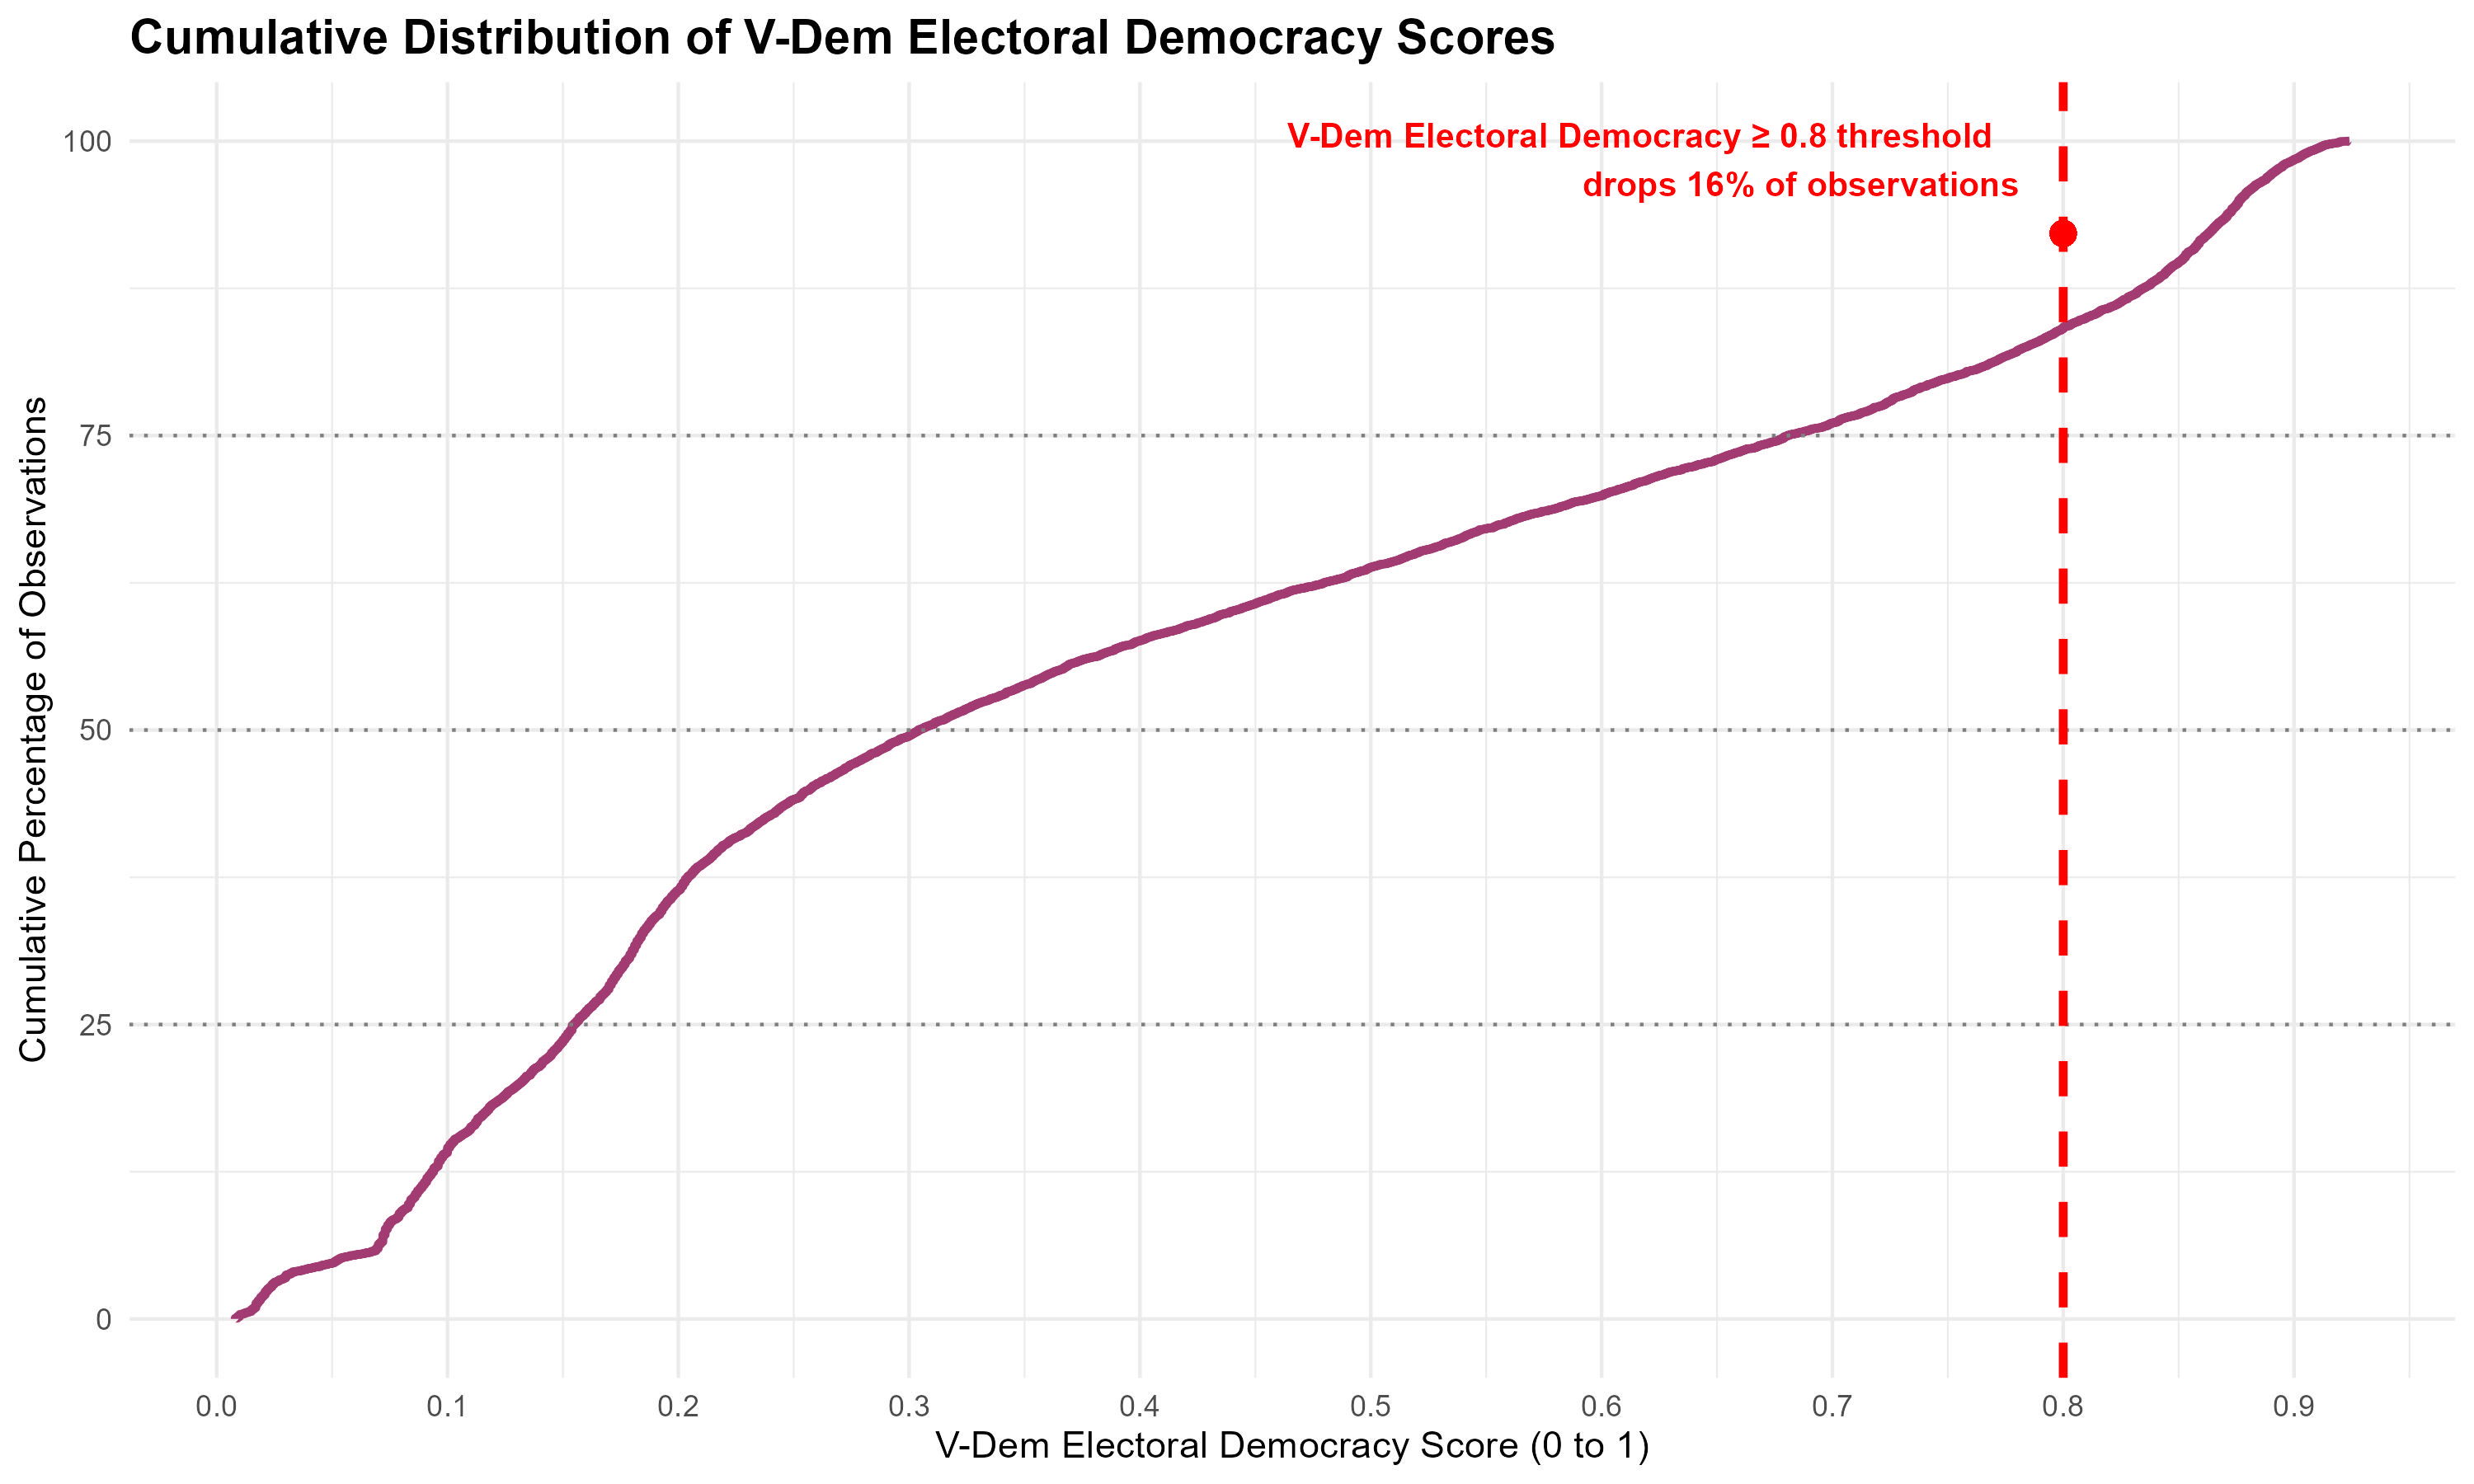
\includegraphics[scale=0.15]{C:/Users/Redha CHABA/Documents/wp_git/cdhm/plots/report/cumul_vdem.jpg}
    \end{center}
\end{figure}

\begin{figure}[H]
    \begin{center}
    \caption{Sample Impact of Democracy Thresholds - Approach 1: Any Observation Above Threshold}
    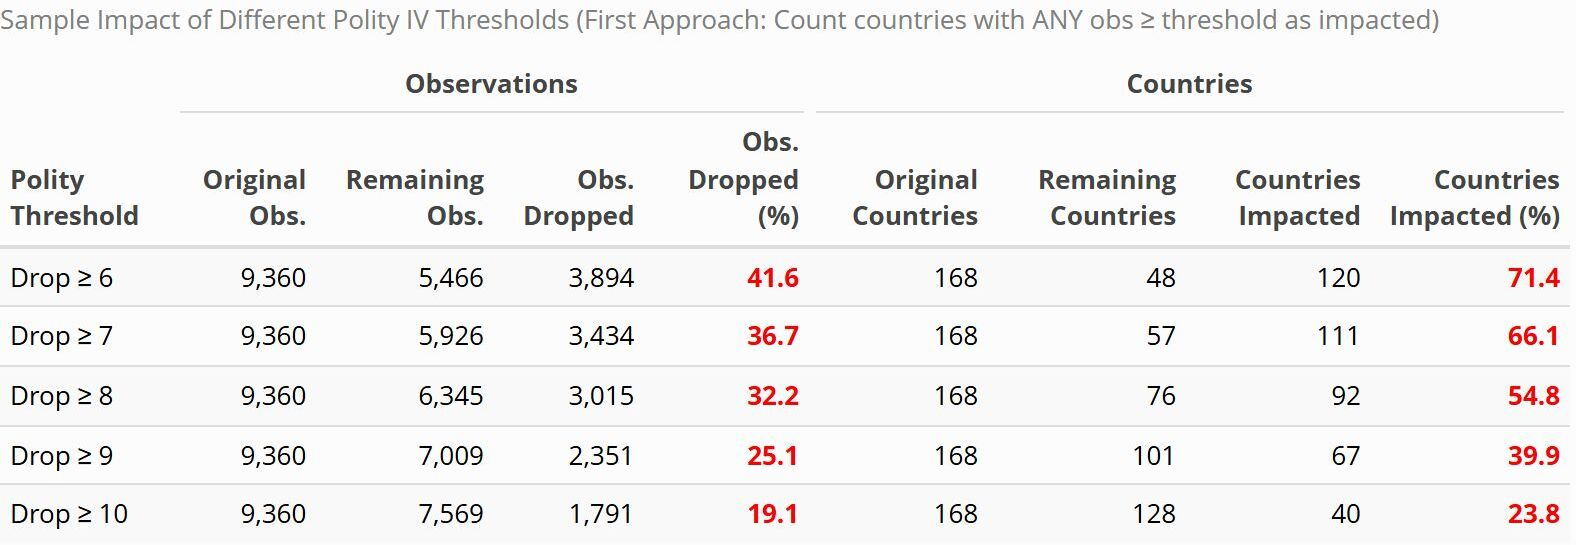
\includegraphics[scale=1.25]{C:/Users/Redha CHABA/Documents/wp_git/cdhm/plots/report/thres_table_polity_1.jpg}
    
    \vspace{1cm}

    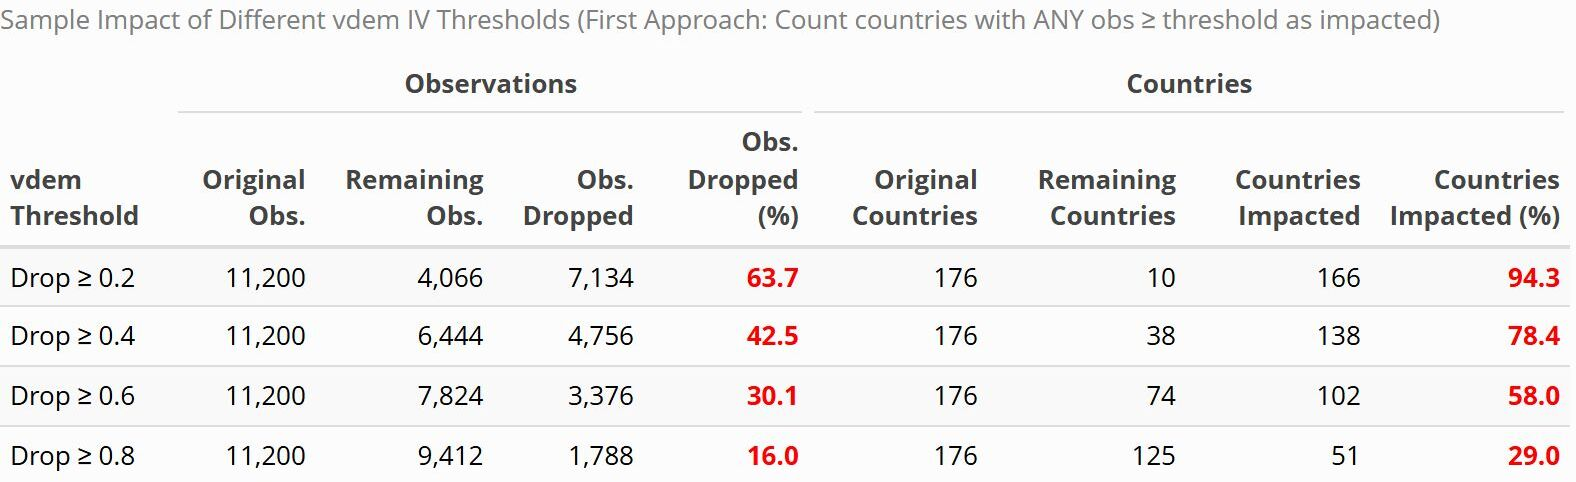
\includegraphics[scale=1.25]{C:/Users/Redha CHABA/Documents/wp_git/cdhm/plots/report/thres_table_vdem_1.jpg}
    
    \end{center}
\end{figure}

\begin{figure}[H]
    \begin{center}
    \caption{Sample Impact of Democracy Thresholds - Approach 2: All Observations Above Threshold}
    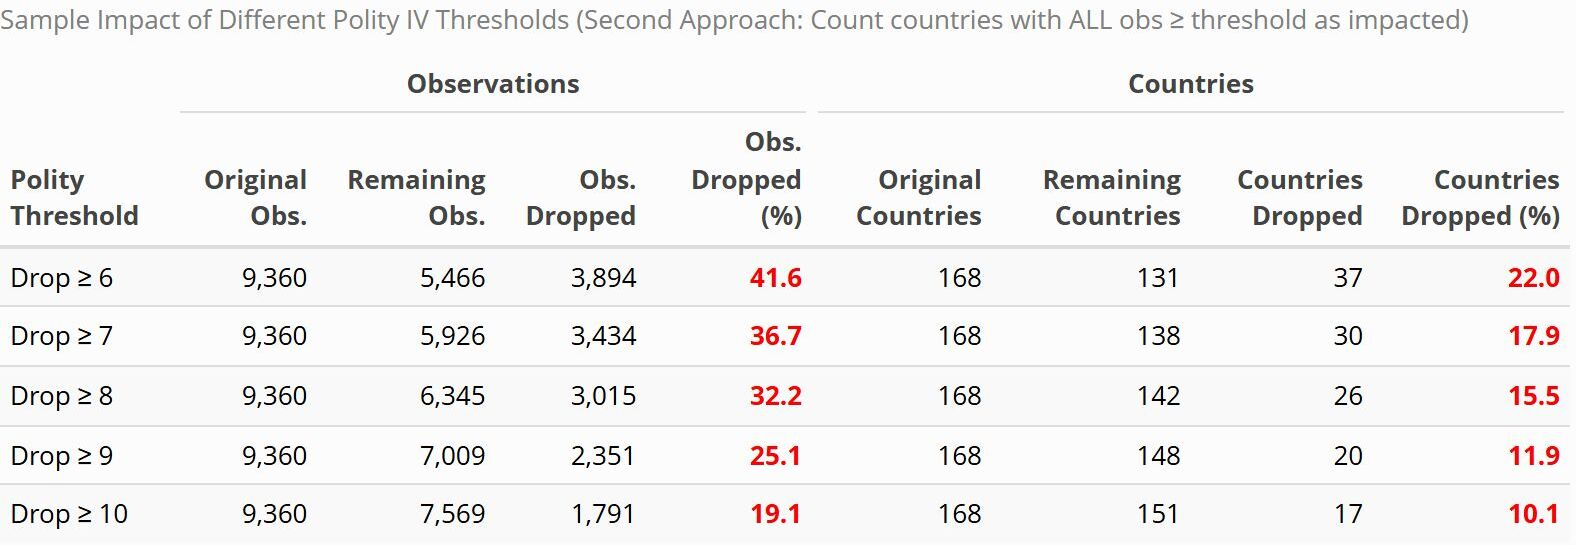
\includegraphics[scale=1.25]{C:/Users/Redha CHABA/Documents/wp_git/cdhm/plots/report/thres_table_polity_2.jpg}
        
    \vspace{1cm}

    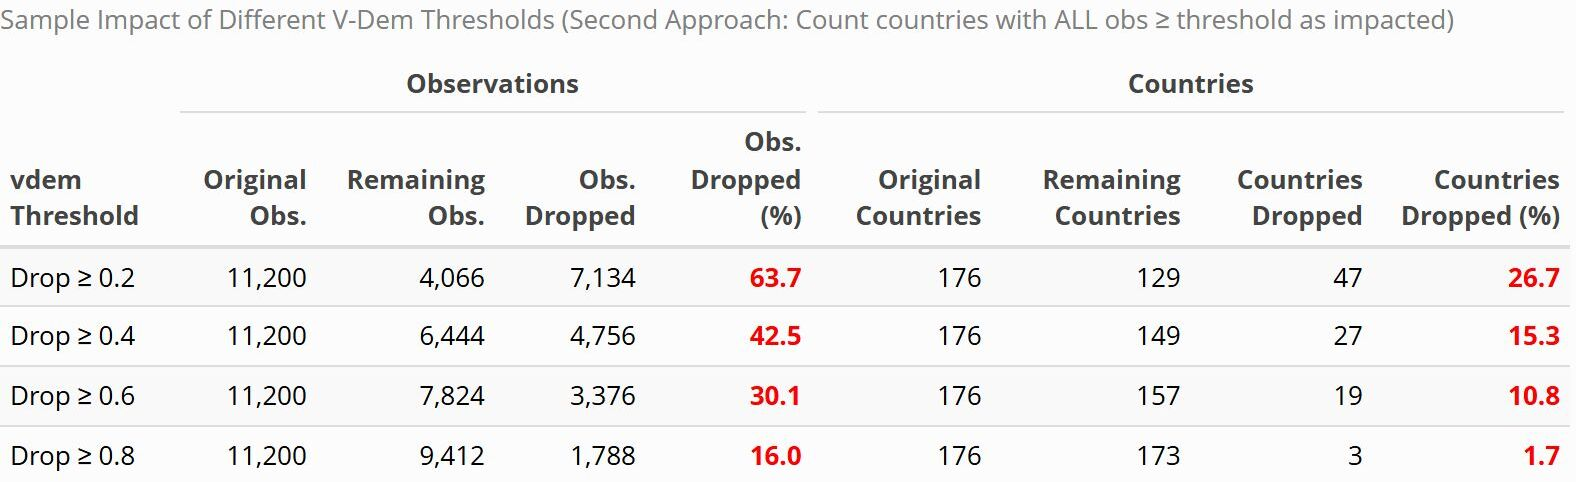
\includegraphics[scale=1.25]{C:/Users/Redha CHABA/Documents/wp_git/cdhm/plots/report/thres_table_vdem_2.jpg}
    \end{center}
\end{figure}

\begin{figure}[H]
    \begin{center}
    \caption{Geographic Distribution - Approach 1: Any Observation Above Threshold}
    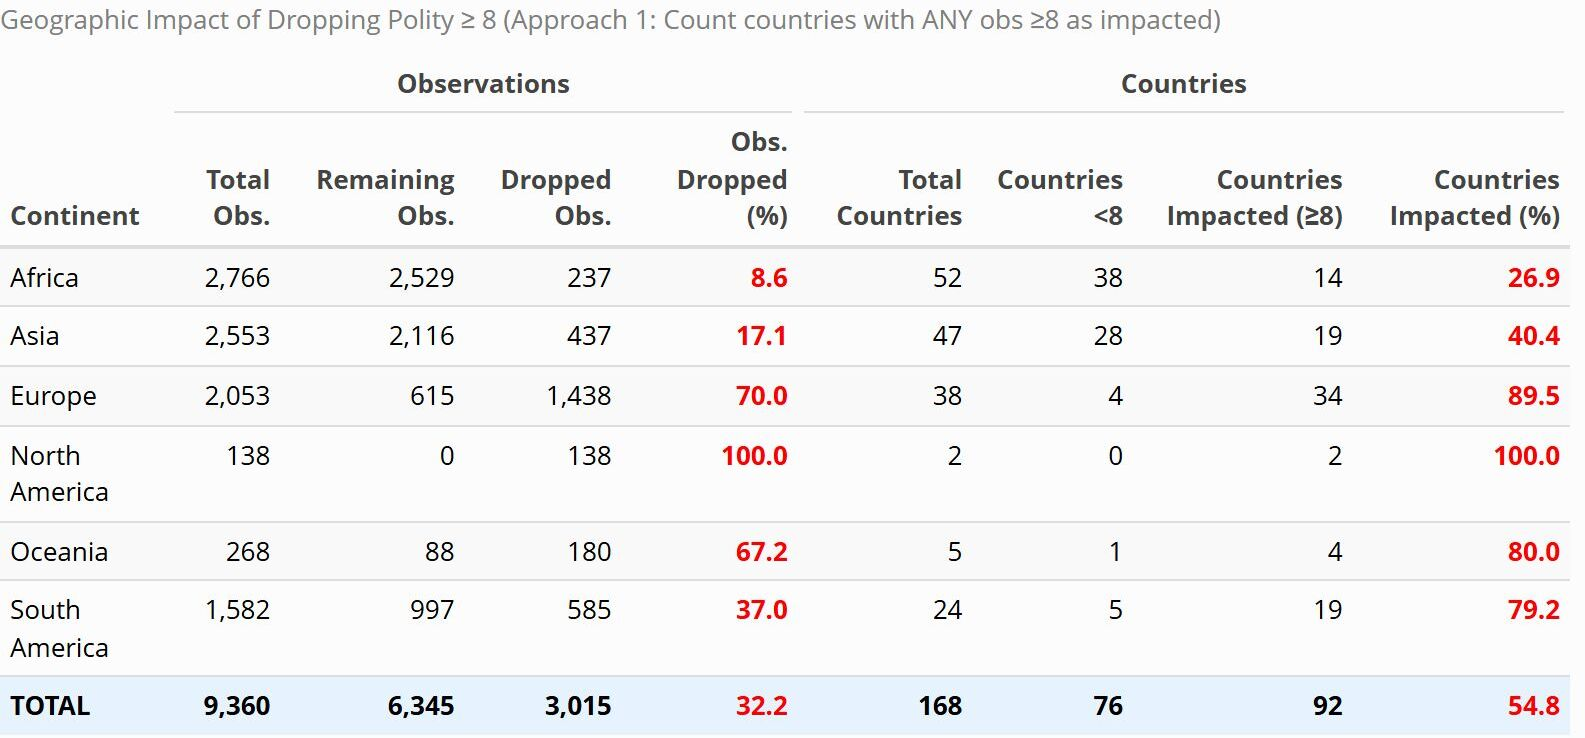
\includegraphics[scale=1.25]{C:/Users/Redha CHABA/Documents/wp_git/cdhm/plots/report/cont_table_polity_1.jpg}
    
    \vspace{1cm}

    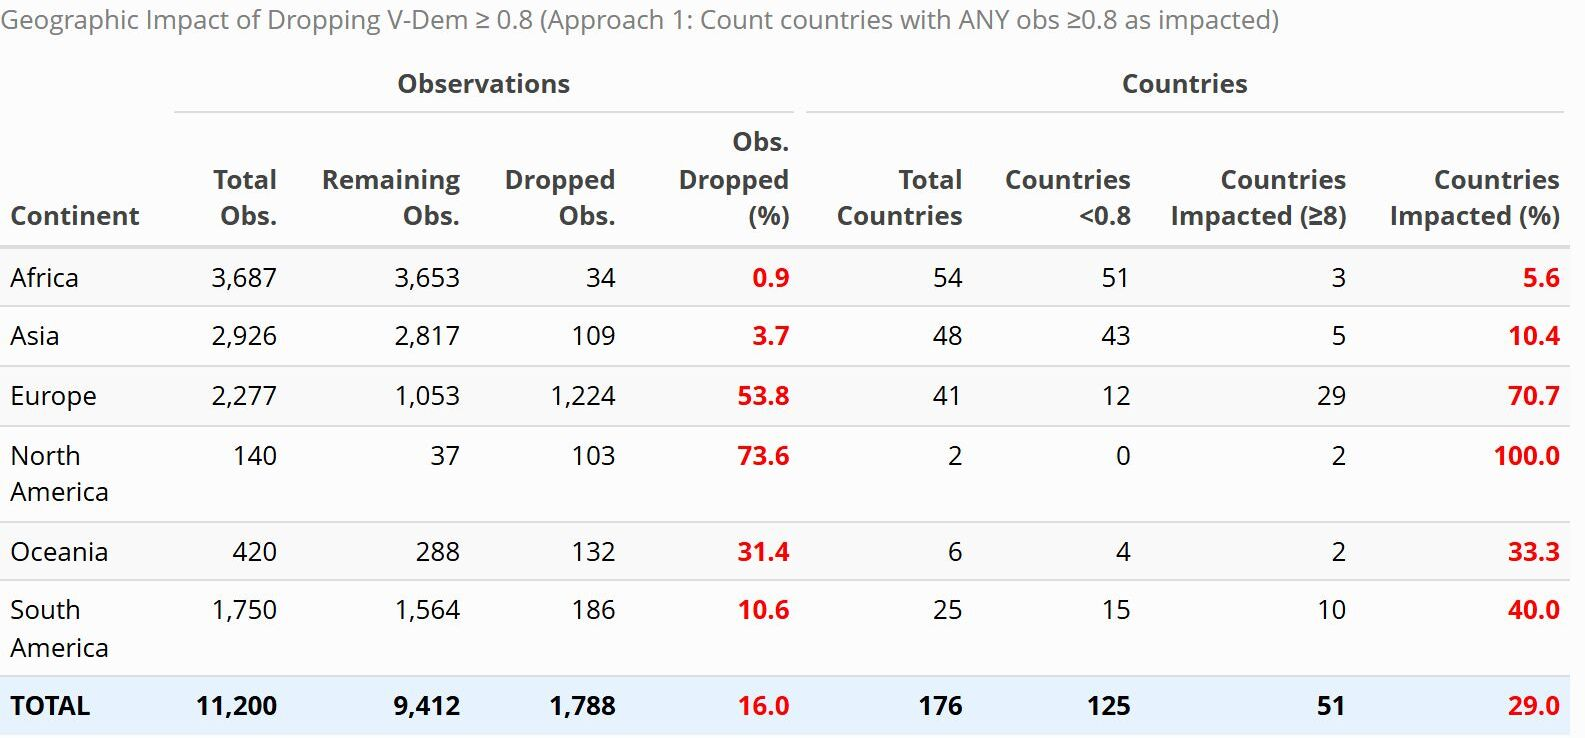
\includegraphics[scale=1.25]{C:/Users/Redha CHABA/Documents/wp_git/cdhm/plots/report/cont_table_vdem_1.jpg}
    \end{center}
\end{figure}

\begin{figure}[H]
    \begin{center}
    \caption{Geographic Distribution - Approach 2: All Observations Above Threshold}
    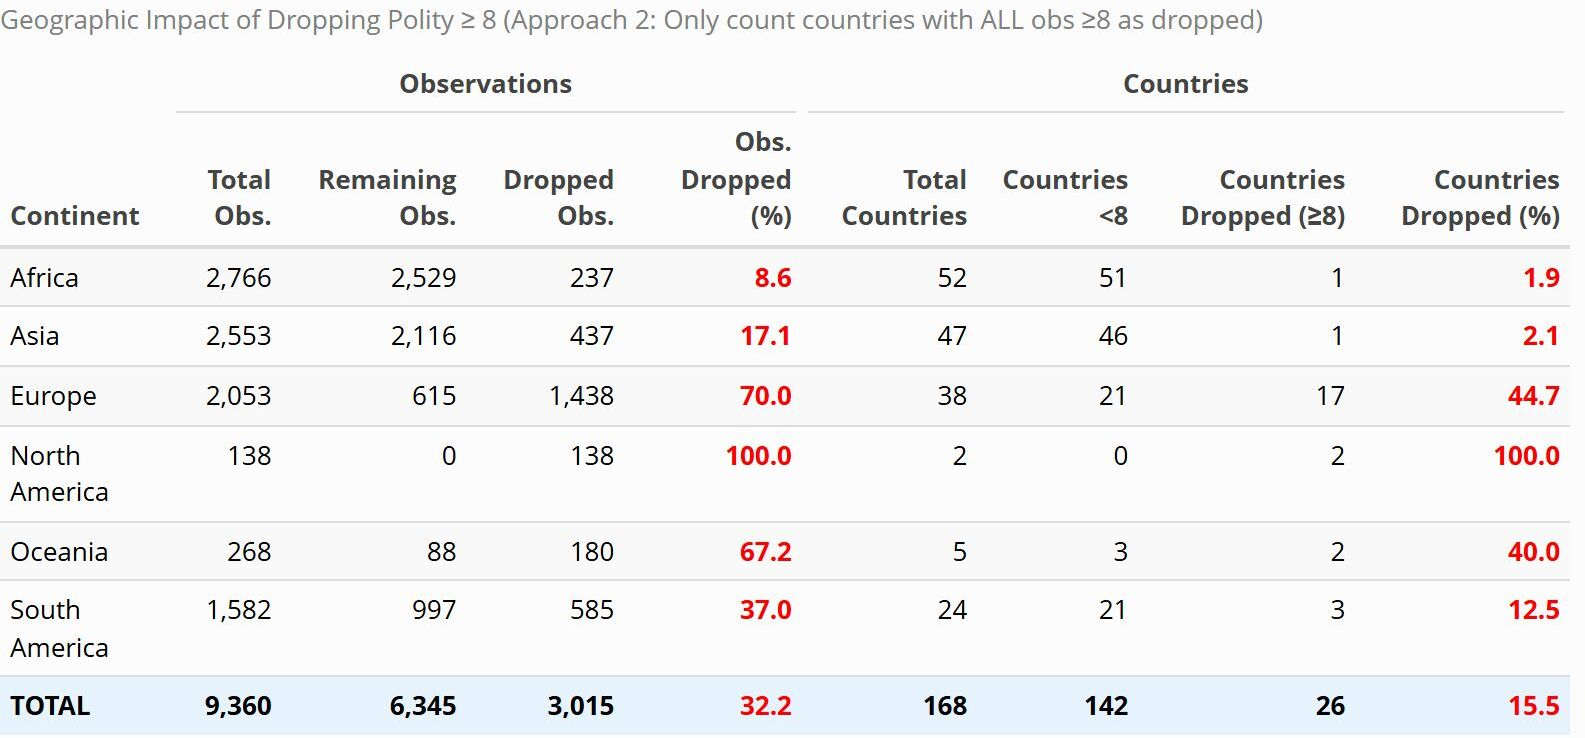
\includegraphics[scale=1.2]{C:/Users/Redha CHABA/Documents/wp_git/cdhm/plots/report/cont_table_polity_2.jpg}

    \vspace{1cm}

    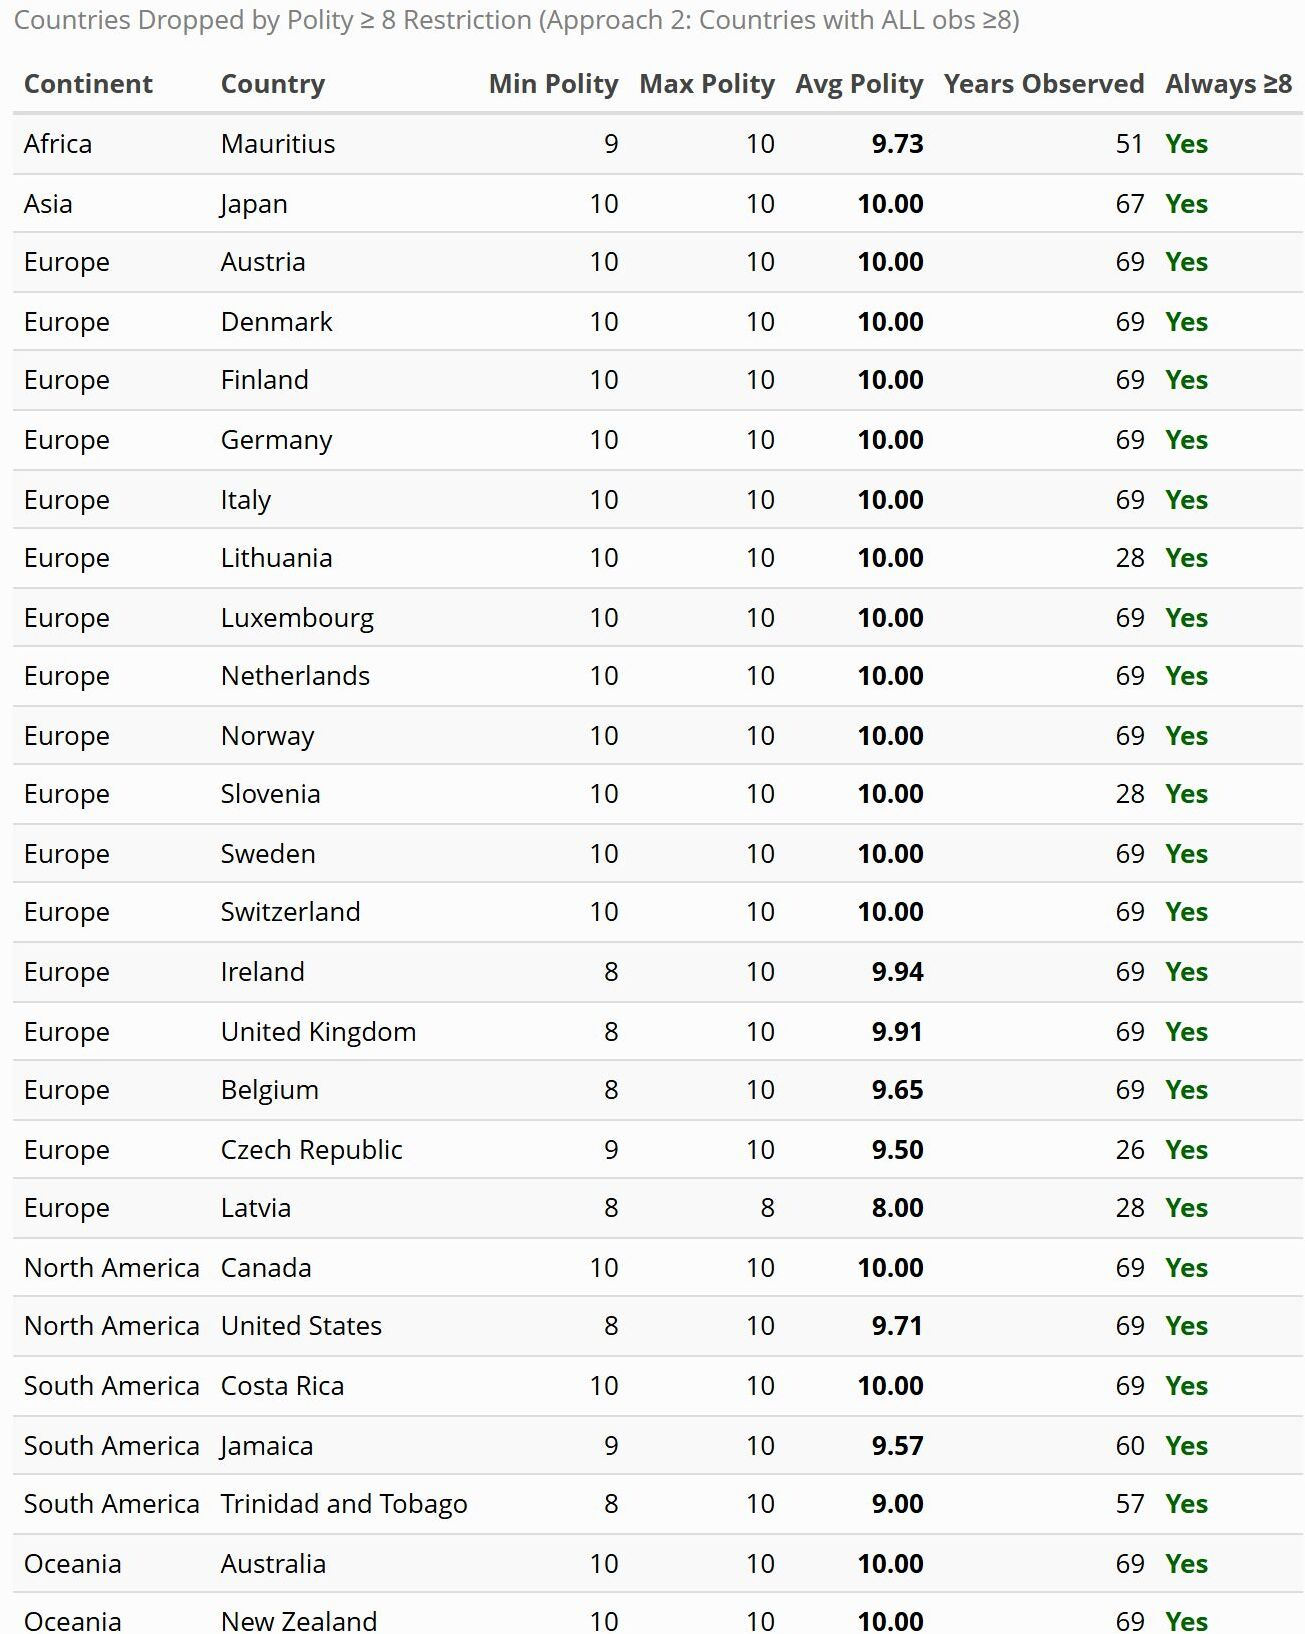
\includegraphics[scale=1.2]{C:/Users/Redha CHABA/Documents/wp_git/cdhm/plots/report/cty_table_polity_2.jpg}
    
    \vspace{1cm}

    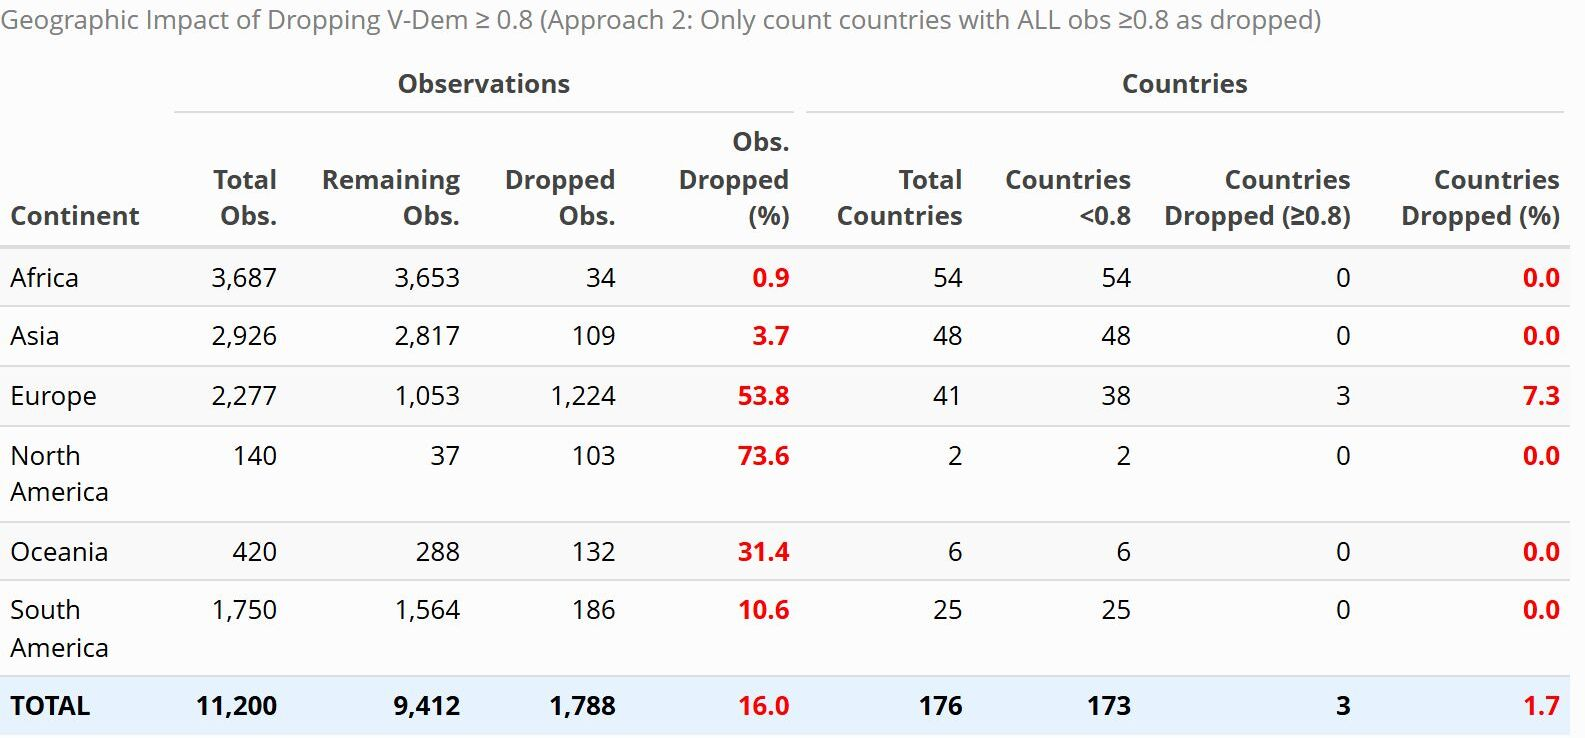
\includegraphics[scale=1.2]{C:/Users/Redha CHABA/Documents/wp_git/cdhm/plots/report/cont_table_vdem_2.jpg}
    \end{center}
\end{figure}

\begin{figure}[H]
    \begin{center}
    \caption{Temporal Patterns - Approach 1: Any Observation Above Threshold}
    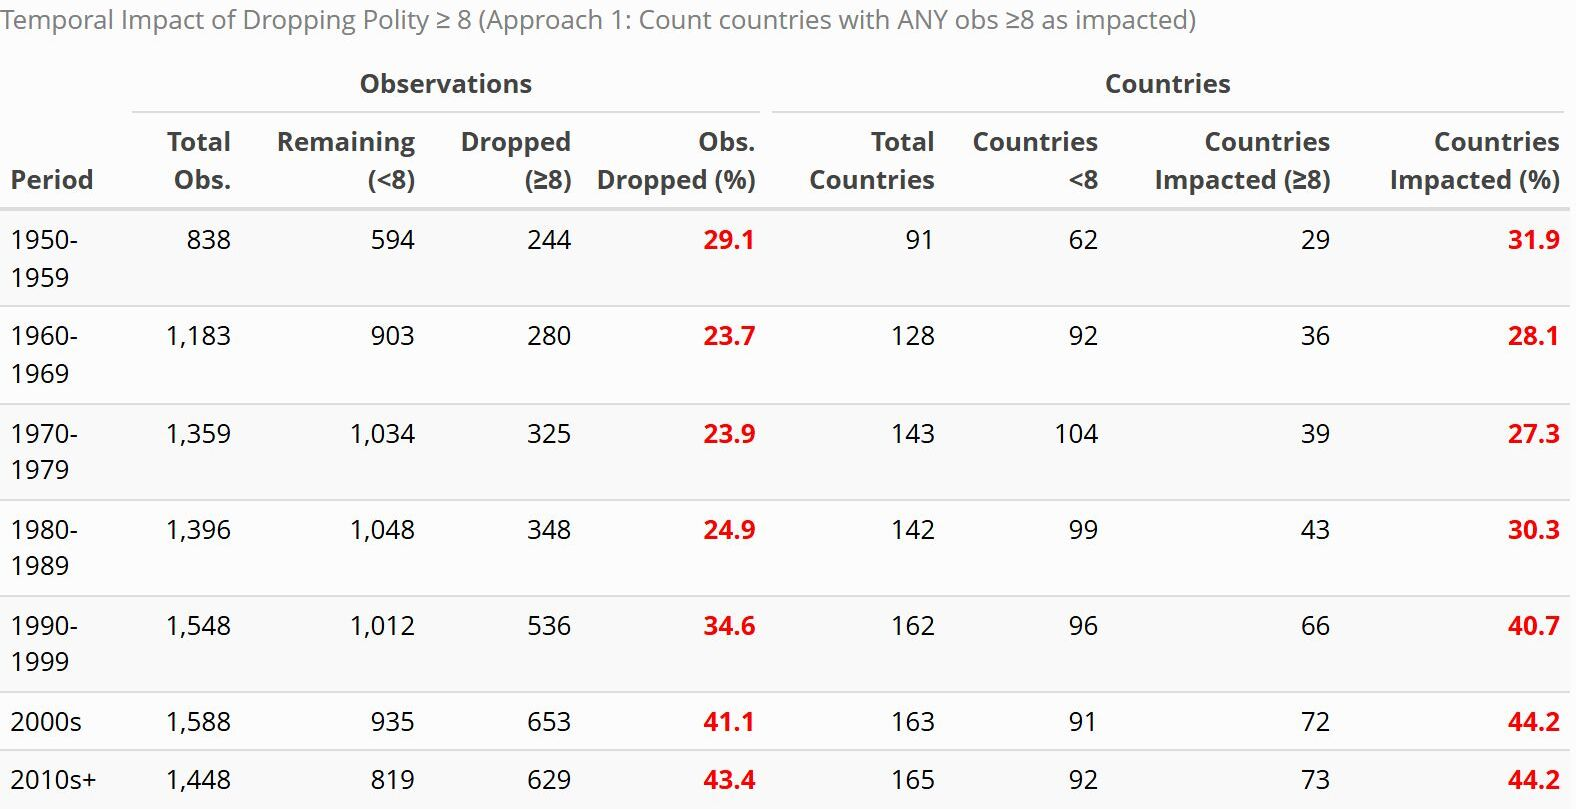
\includegraphics[scale=1.25]{C:/Users/Redha CHABA/Documents/wp_git/cdhm/plots/report/time_table_polity_1.jpg}
        
    \vspace{1cm}

    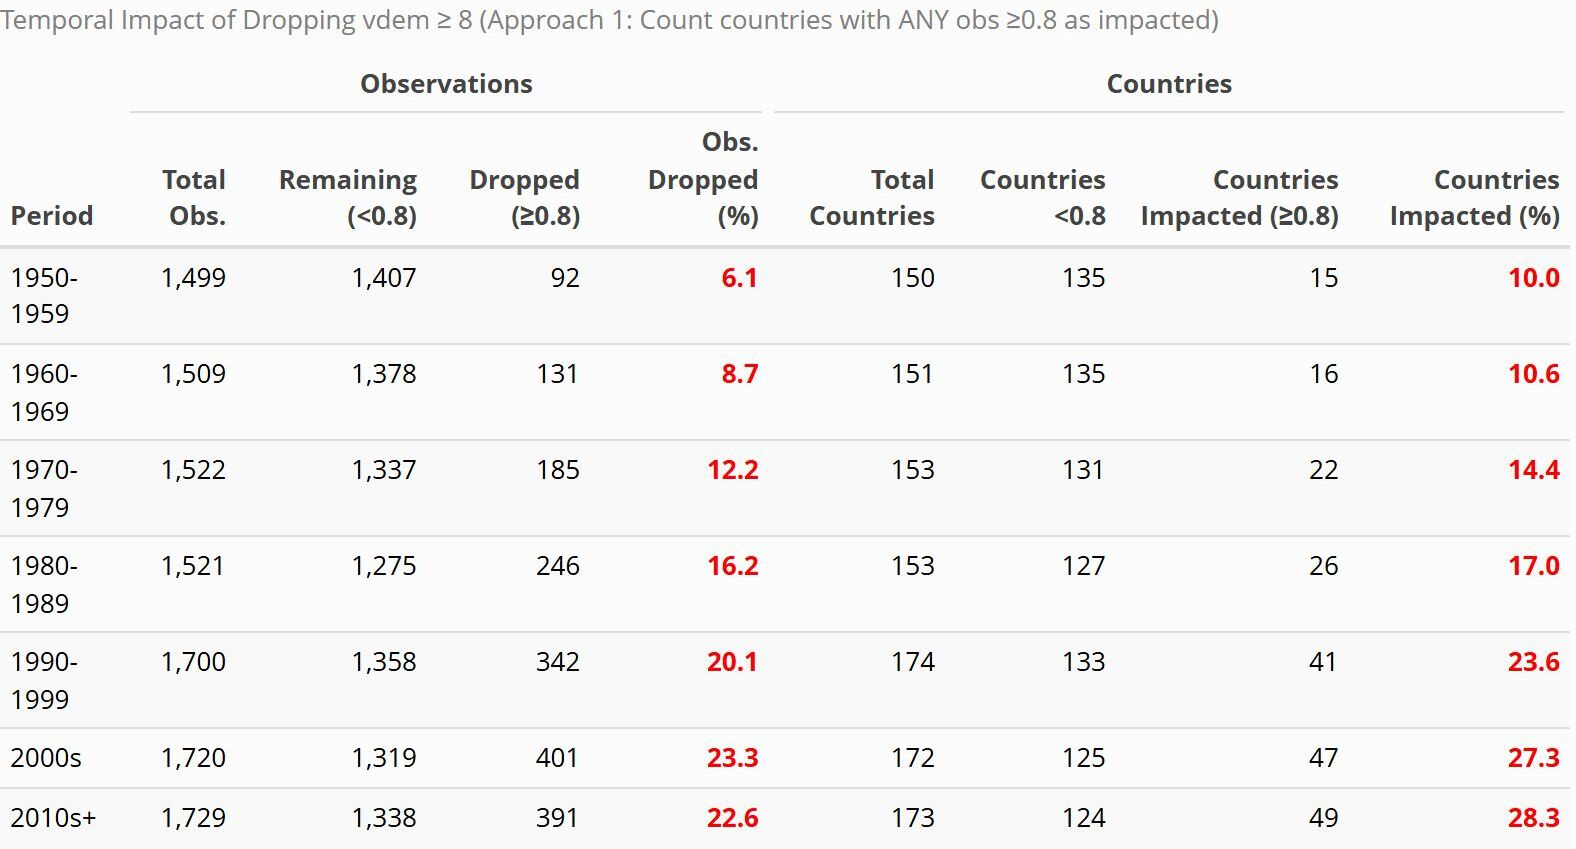
\includegraphics[scale=1.25]{C:/Users/Redha CHABA/Documents/wp_git/cdhm/plots/report/time_table_vdem_1.jpg}
    \end{center}
\end{figure}

\begin{figure}[H]
    \begin{center}
    \caption{Temporal Patterns - Approach 2: All Observations Above Threshold}
    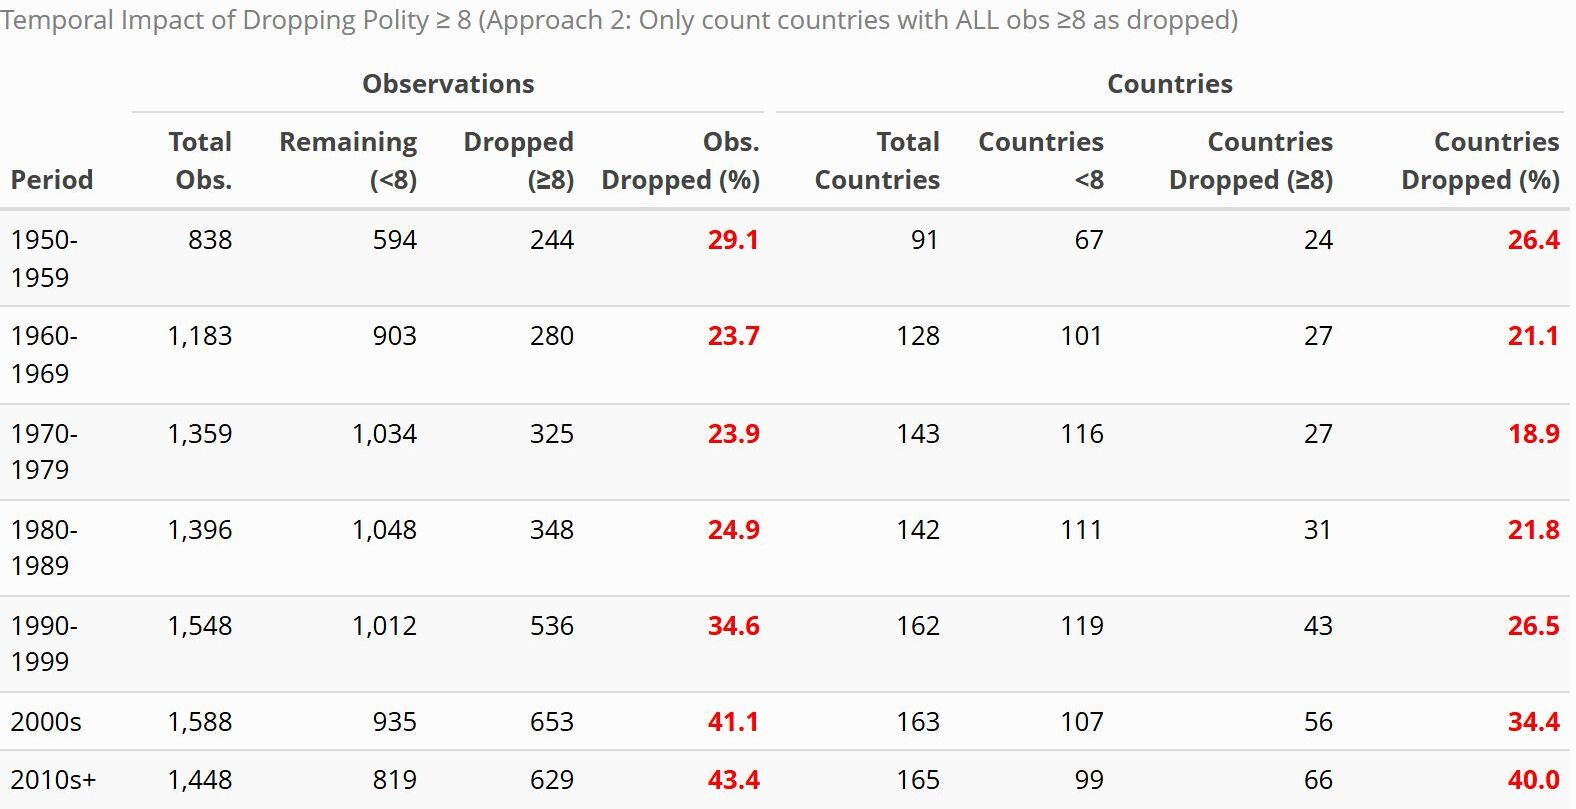
\includegraphics[scale=1.25]{C:/Users/Redha CHABA/Documents/wp_git/cdhm/plots/report/time_table_polity_2.jpg}
    
    \vspace{1cm}

    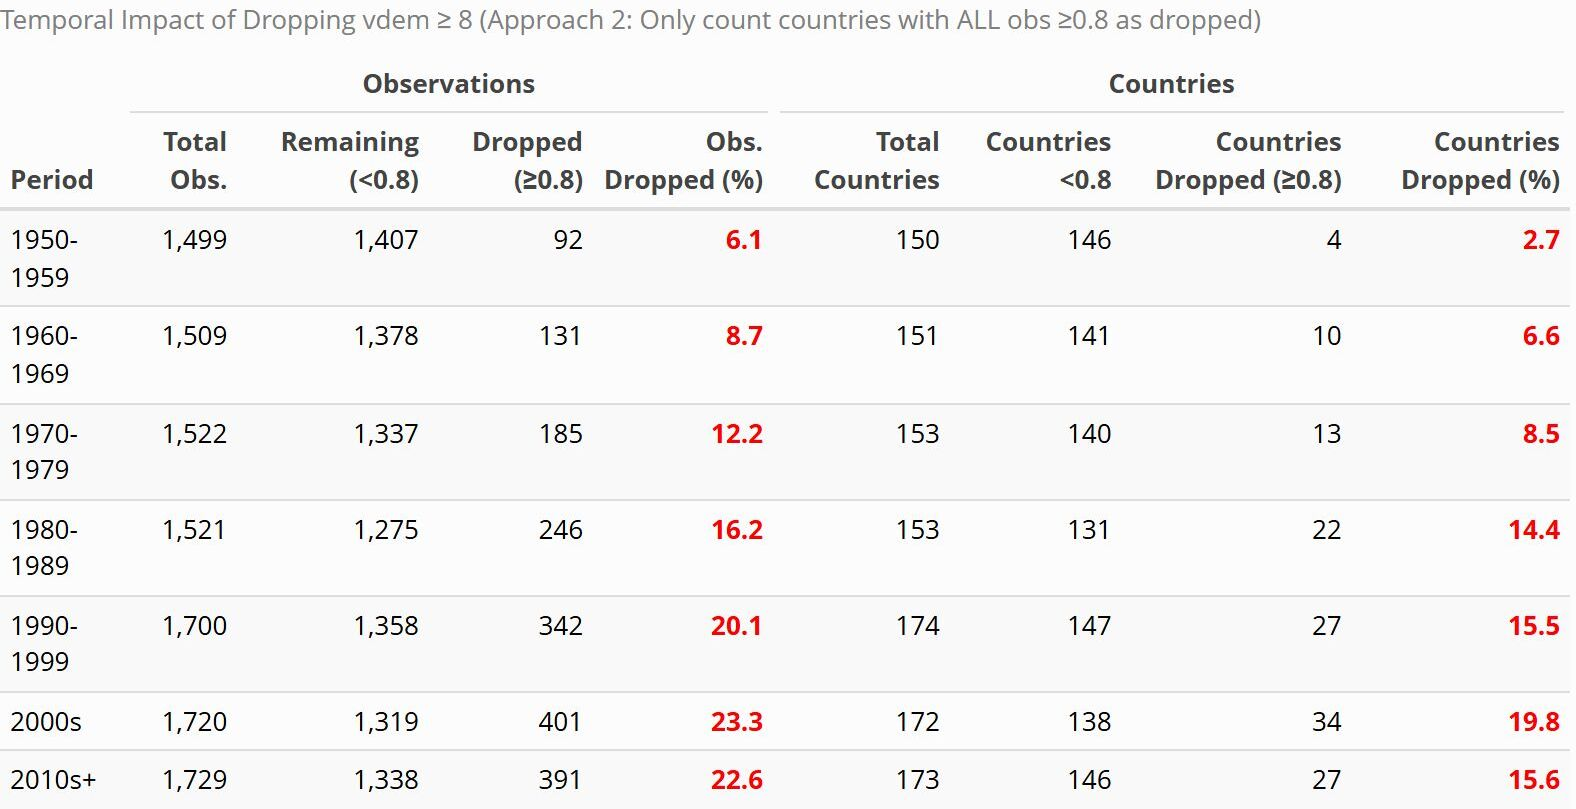
\includegraphics[scale=1.25]{C:/Users/Redha CHABA/Documents/wp_git/cdhm/plots/report/time_table_vdem_2.jpg}
    
    \end{center}
\end{figure}


\end{document}
